\section{Horseshoe model MCMC convergence} \label{app:horseshoe_convergence}
This appendix collects the diagnostics behind the convergence claims made in
Section~\ref{sec:regression} for the horseshoe model. Three chains,
\num{30000} retained draws each after a burn-in of \num{1000} and thinning of
$3$. Diagnostics are reported separately for the two blocks of parameters:
the regression coefficients $\{\beta_j, \beta_0, \beta_{\text{mid}}\}$ and the
scale parameters $\{\lambda_j, \lambda_{\text{mid}}, \tau\}$, the latter being
the harder to sample.

\subsection*{Trace plots}
Figures~\ref{fig:hs_trace_beta} and~\ref{fig:hs_trace_lambda} in
Section~\ref{sec:regression} show the first group of each block. The remaining
groups follow.
\begin{figure}[htbp]
  \centering
  \begin{subfigure}[t]{0.48\linewidth}
    \centering
    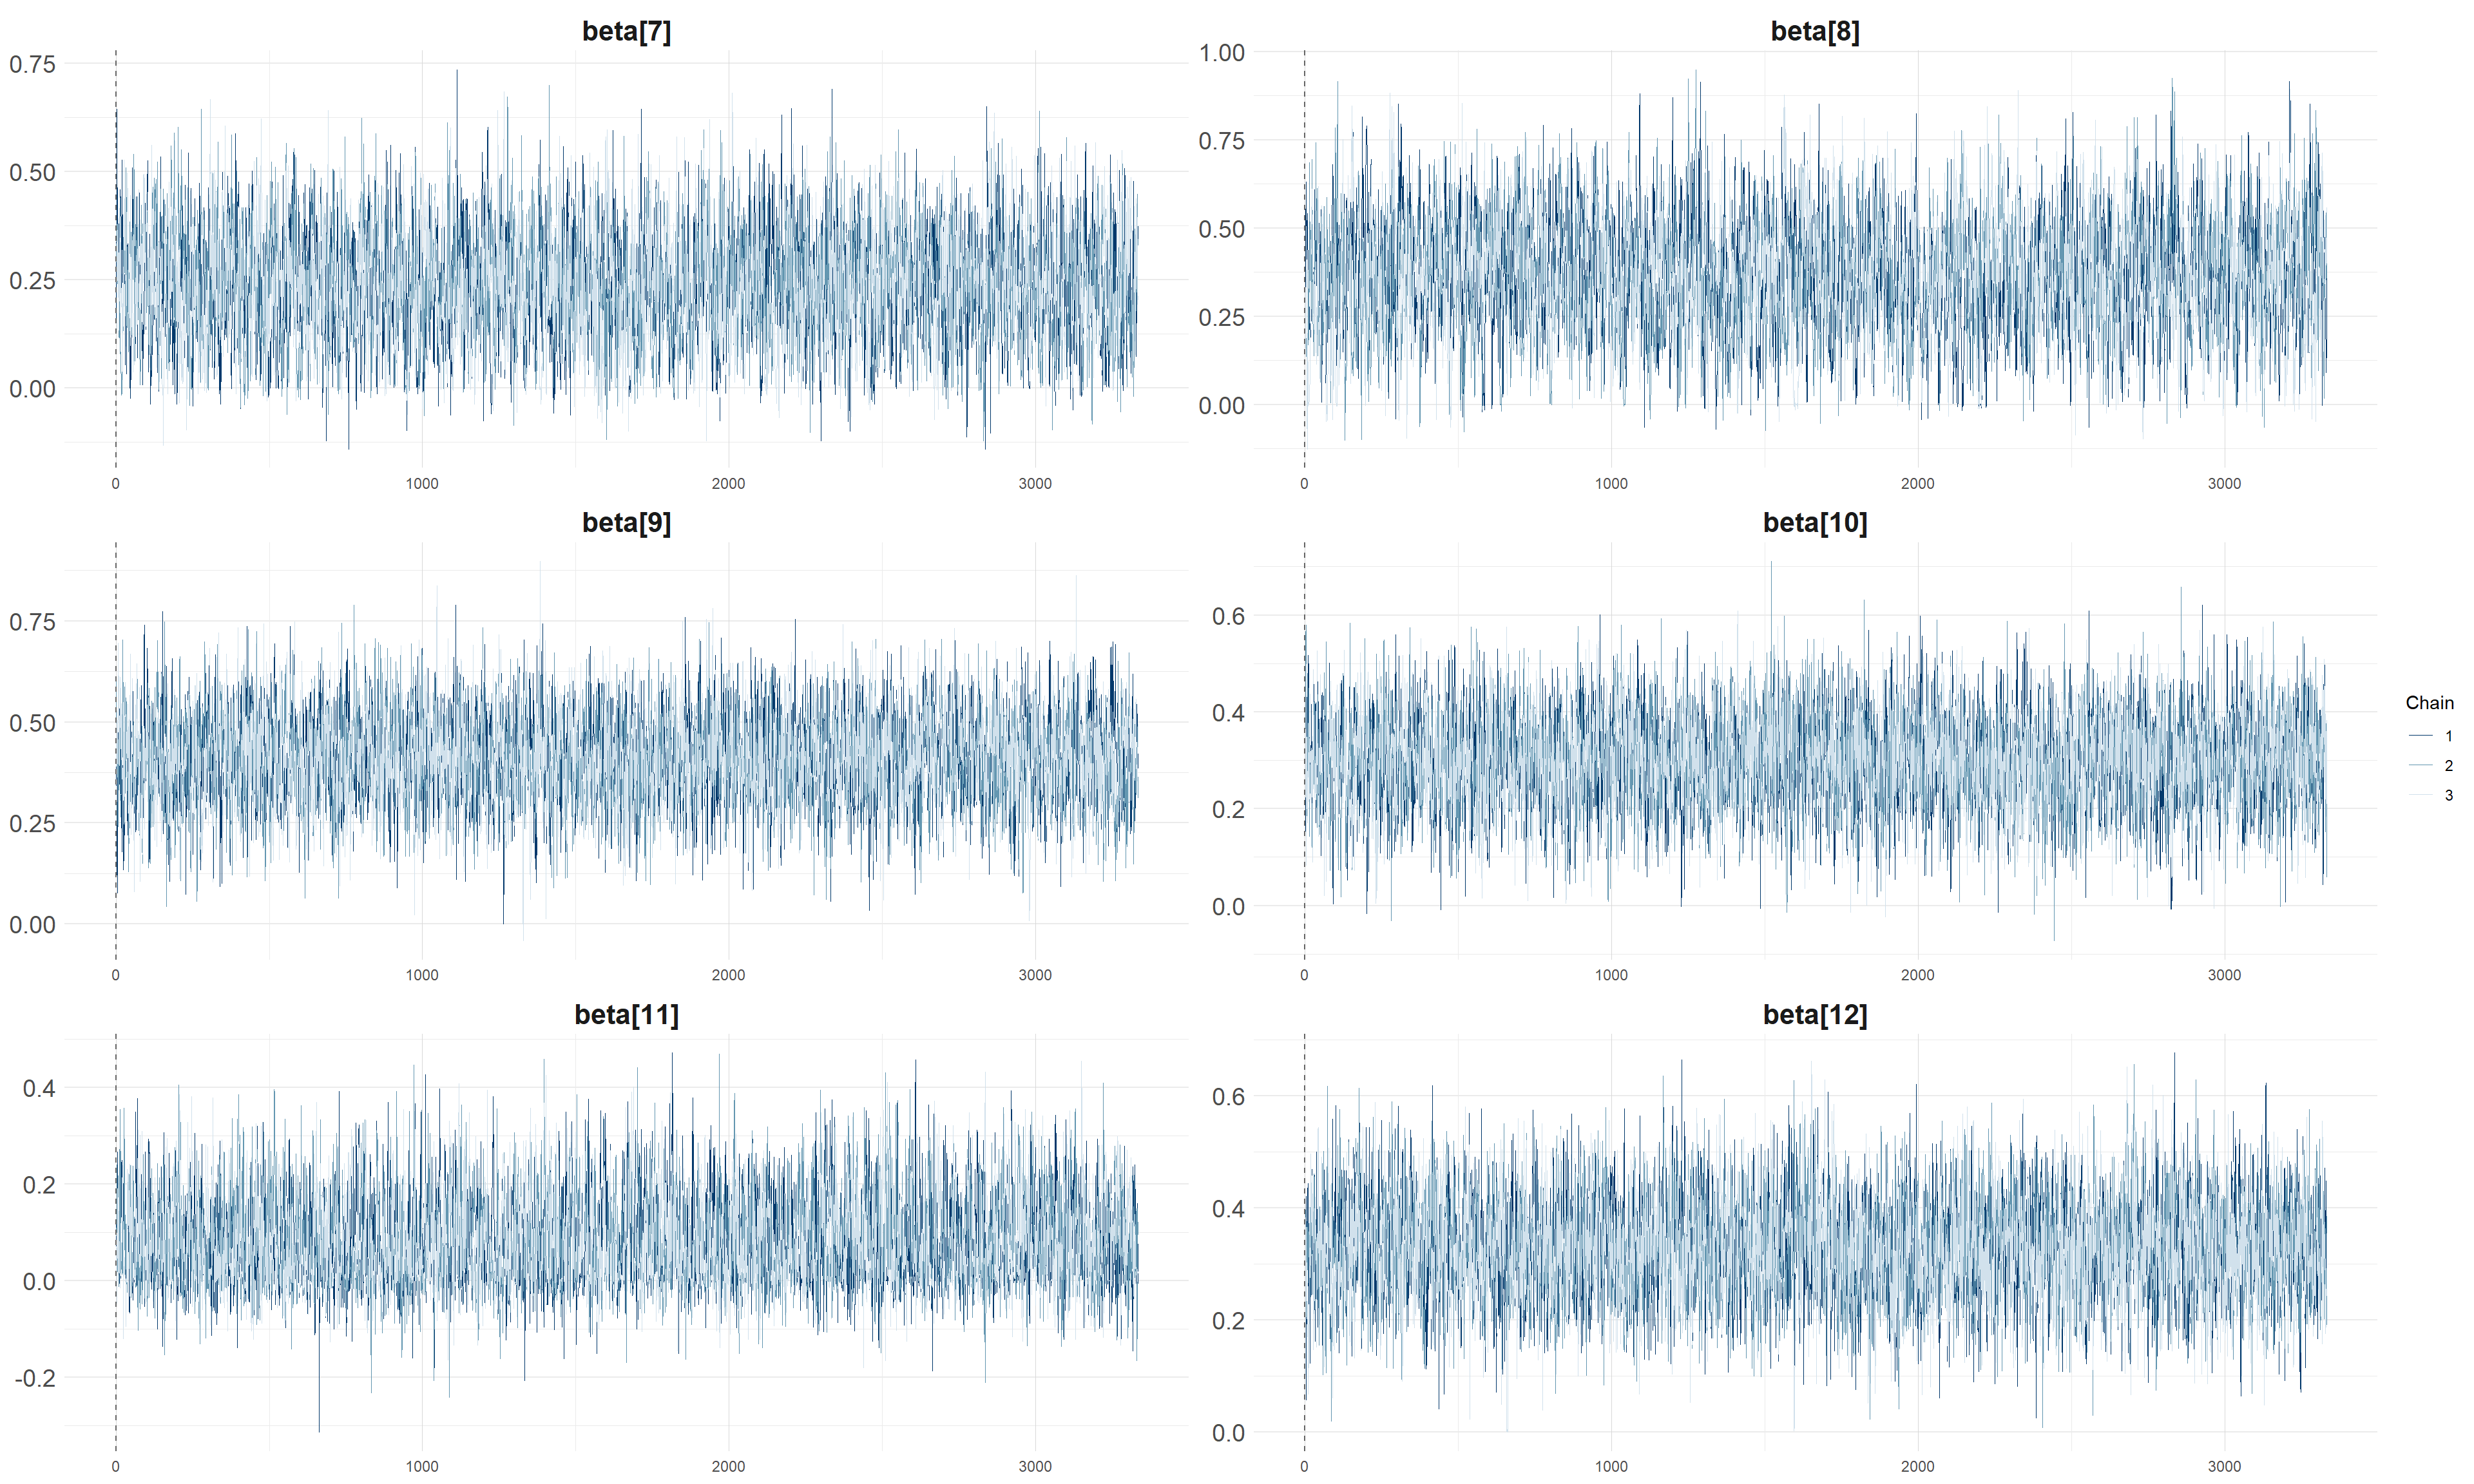
\includegraphics[width=\linewidth]{img/horseshoe_model/trace_beta_2.png}
    \caption{Group 2.}
  \end{subfigure}\hfill
  \begin{subfigure}[t]{0.48\linewidth}
    \centering
    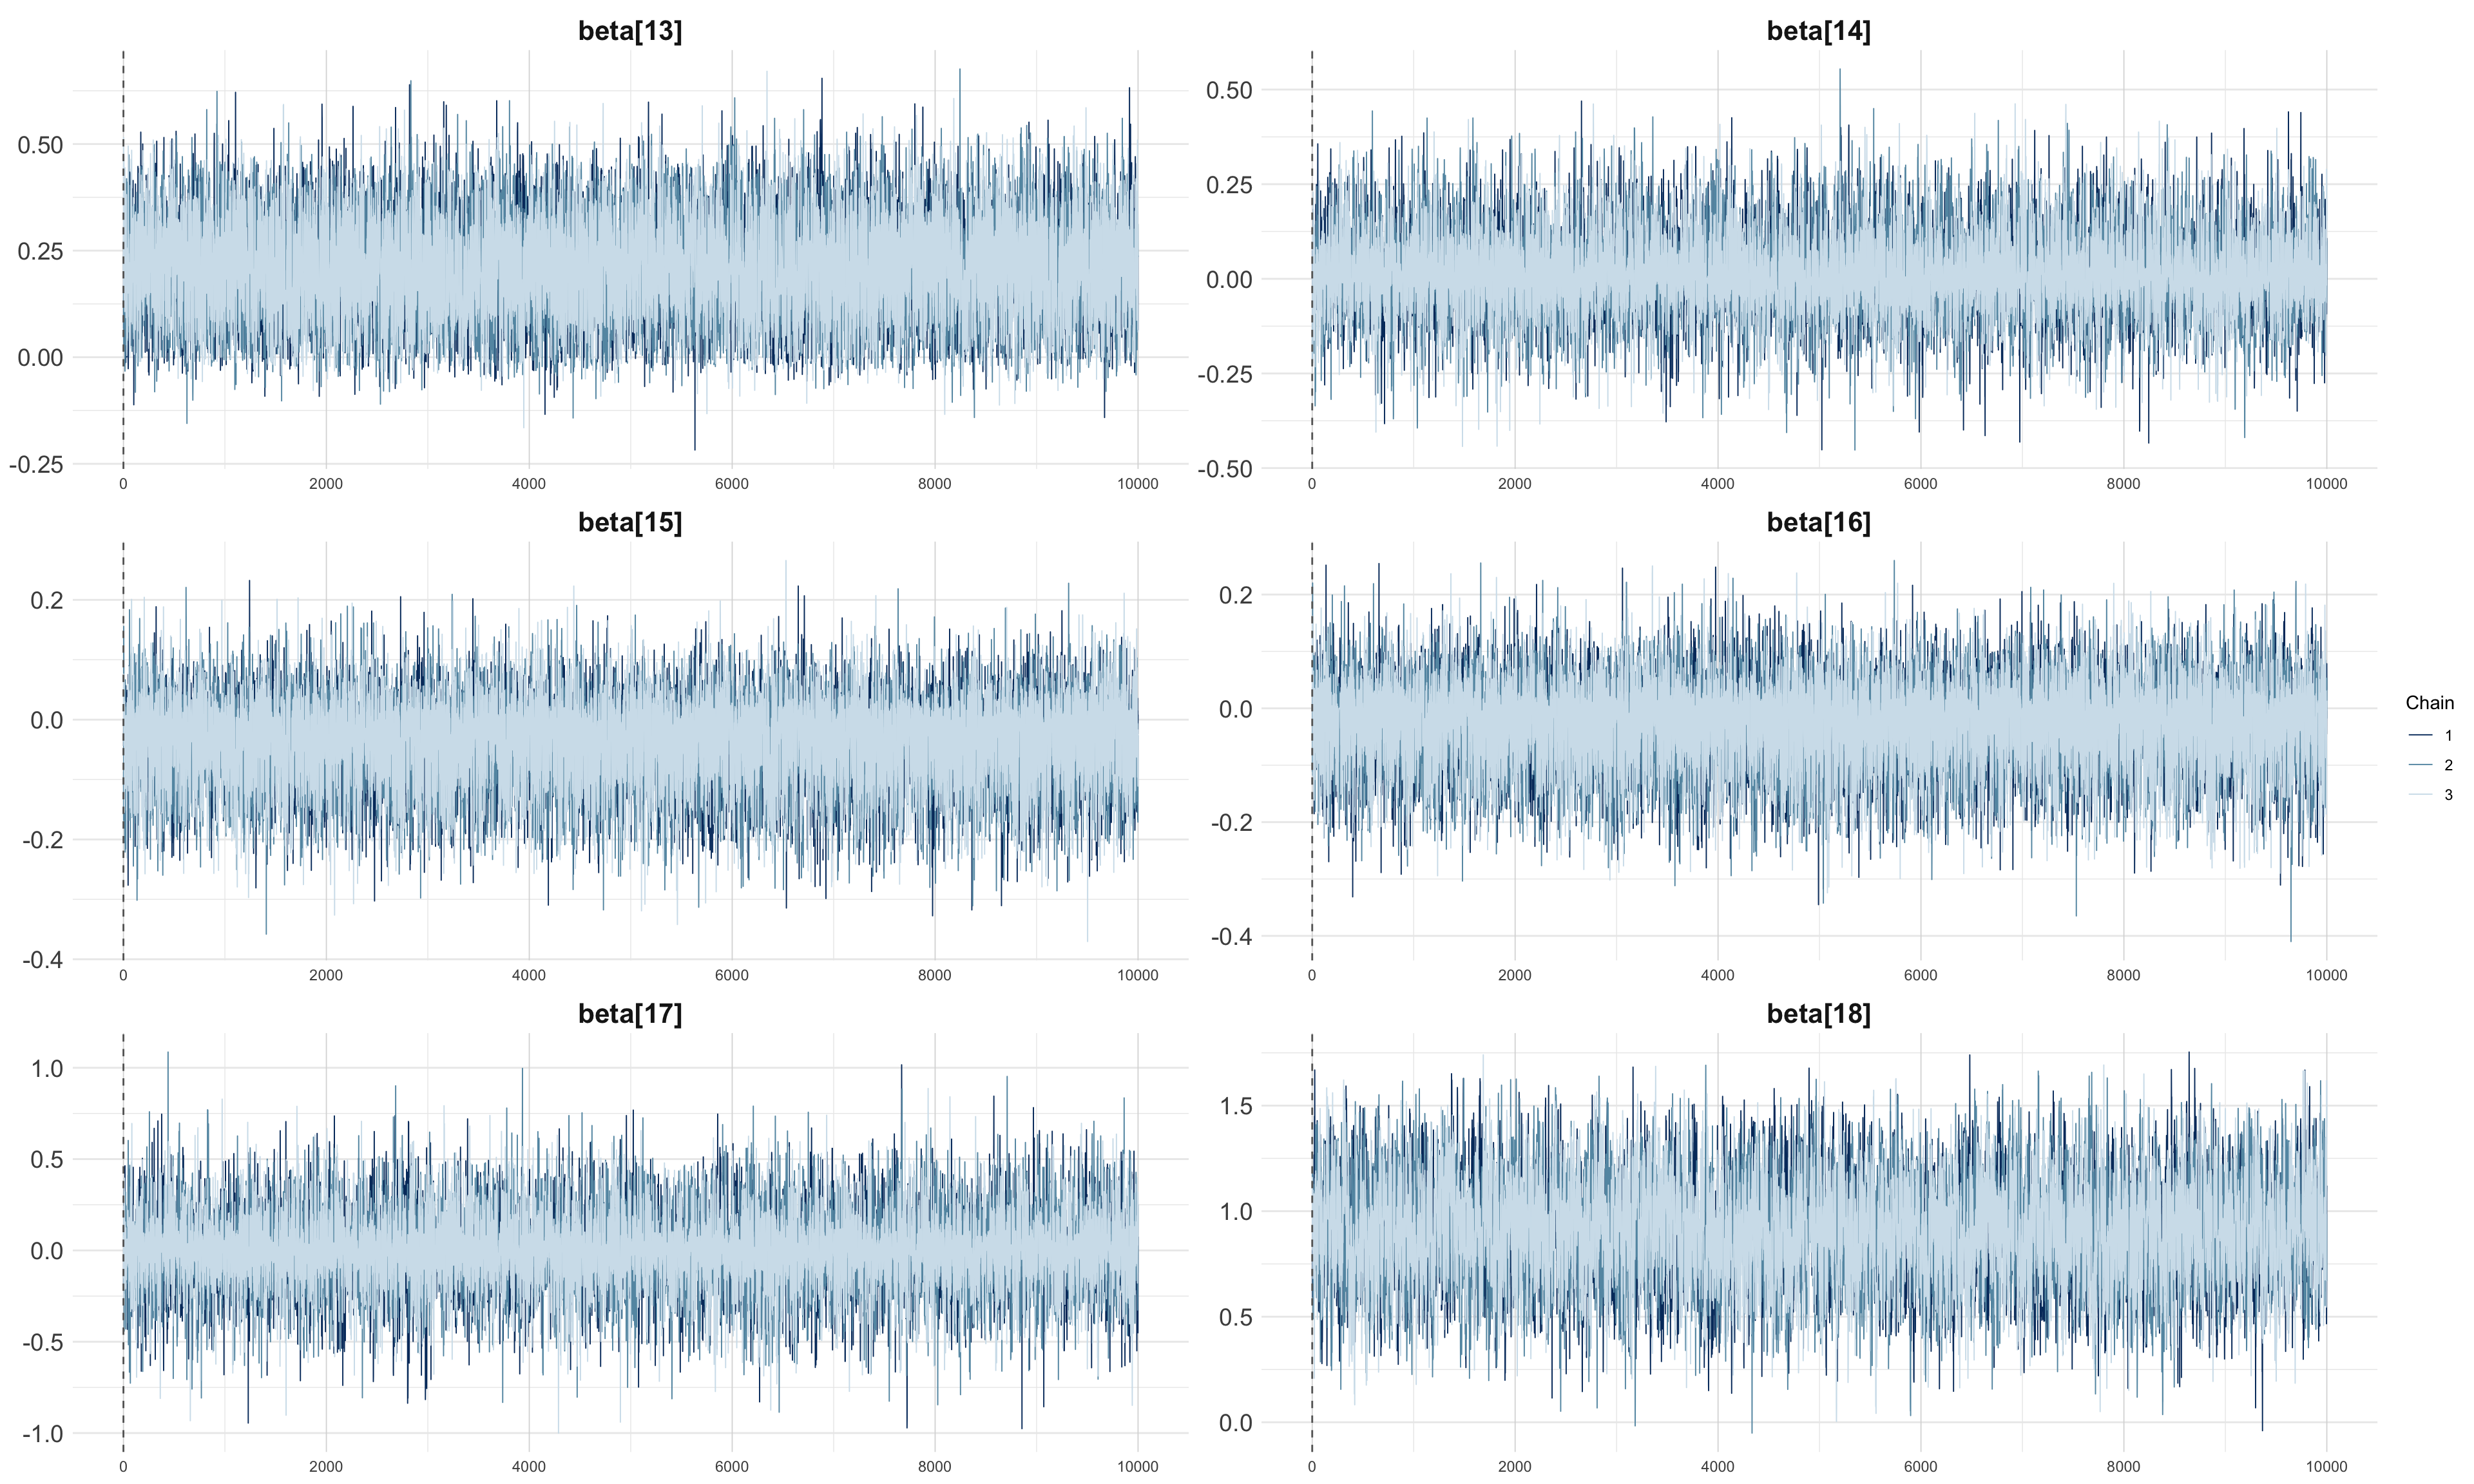
\includegraphics[width=\linewidth]{img/horseshoe_model/trace_beta_3.png}
    \caption{Group 3.}
  \end{subfigure}\hfill
  \begin{subfigure}[t]{0.48\linewidth}
    \centering
    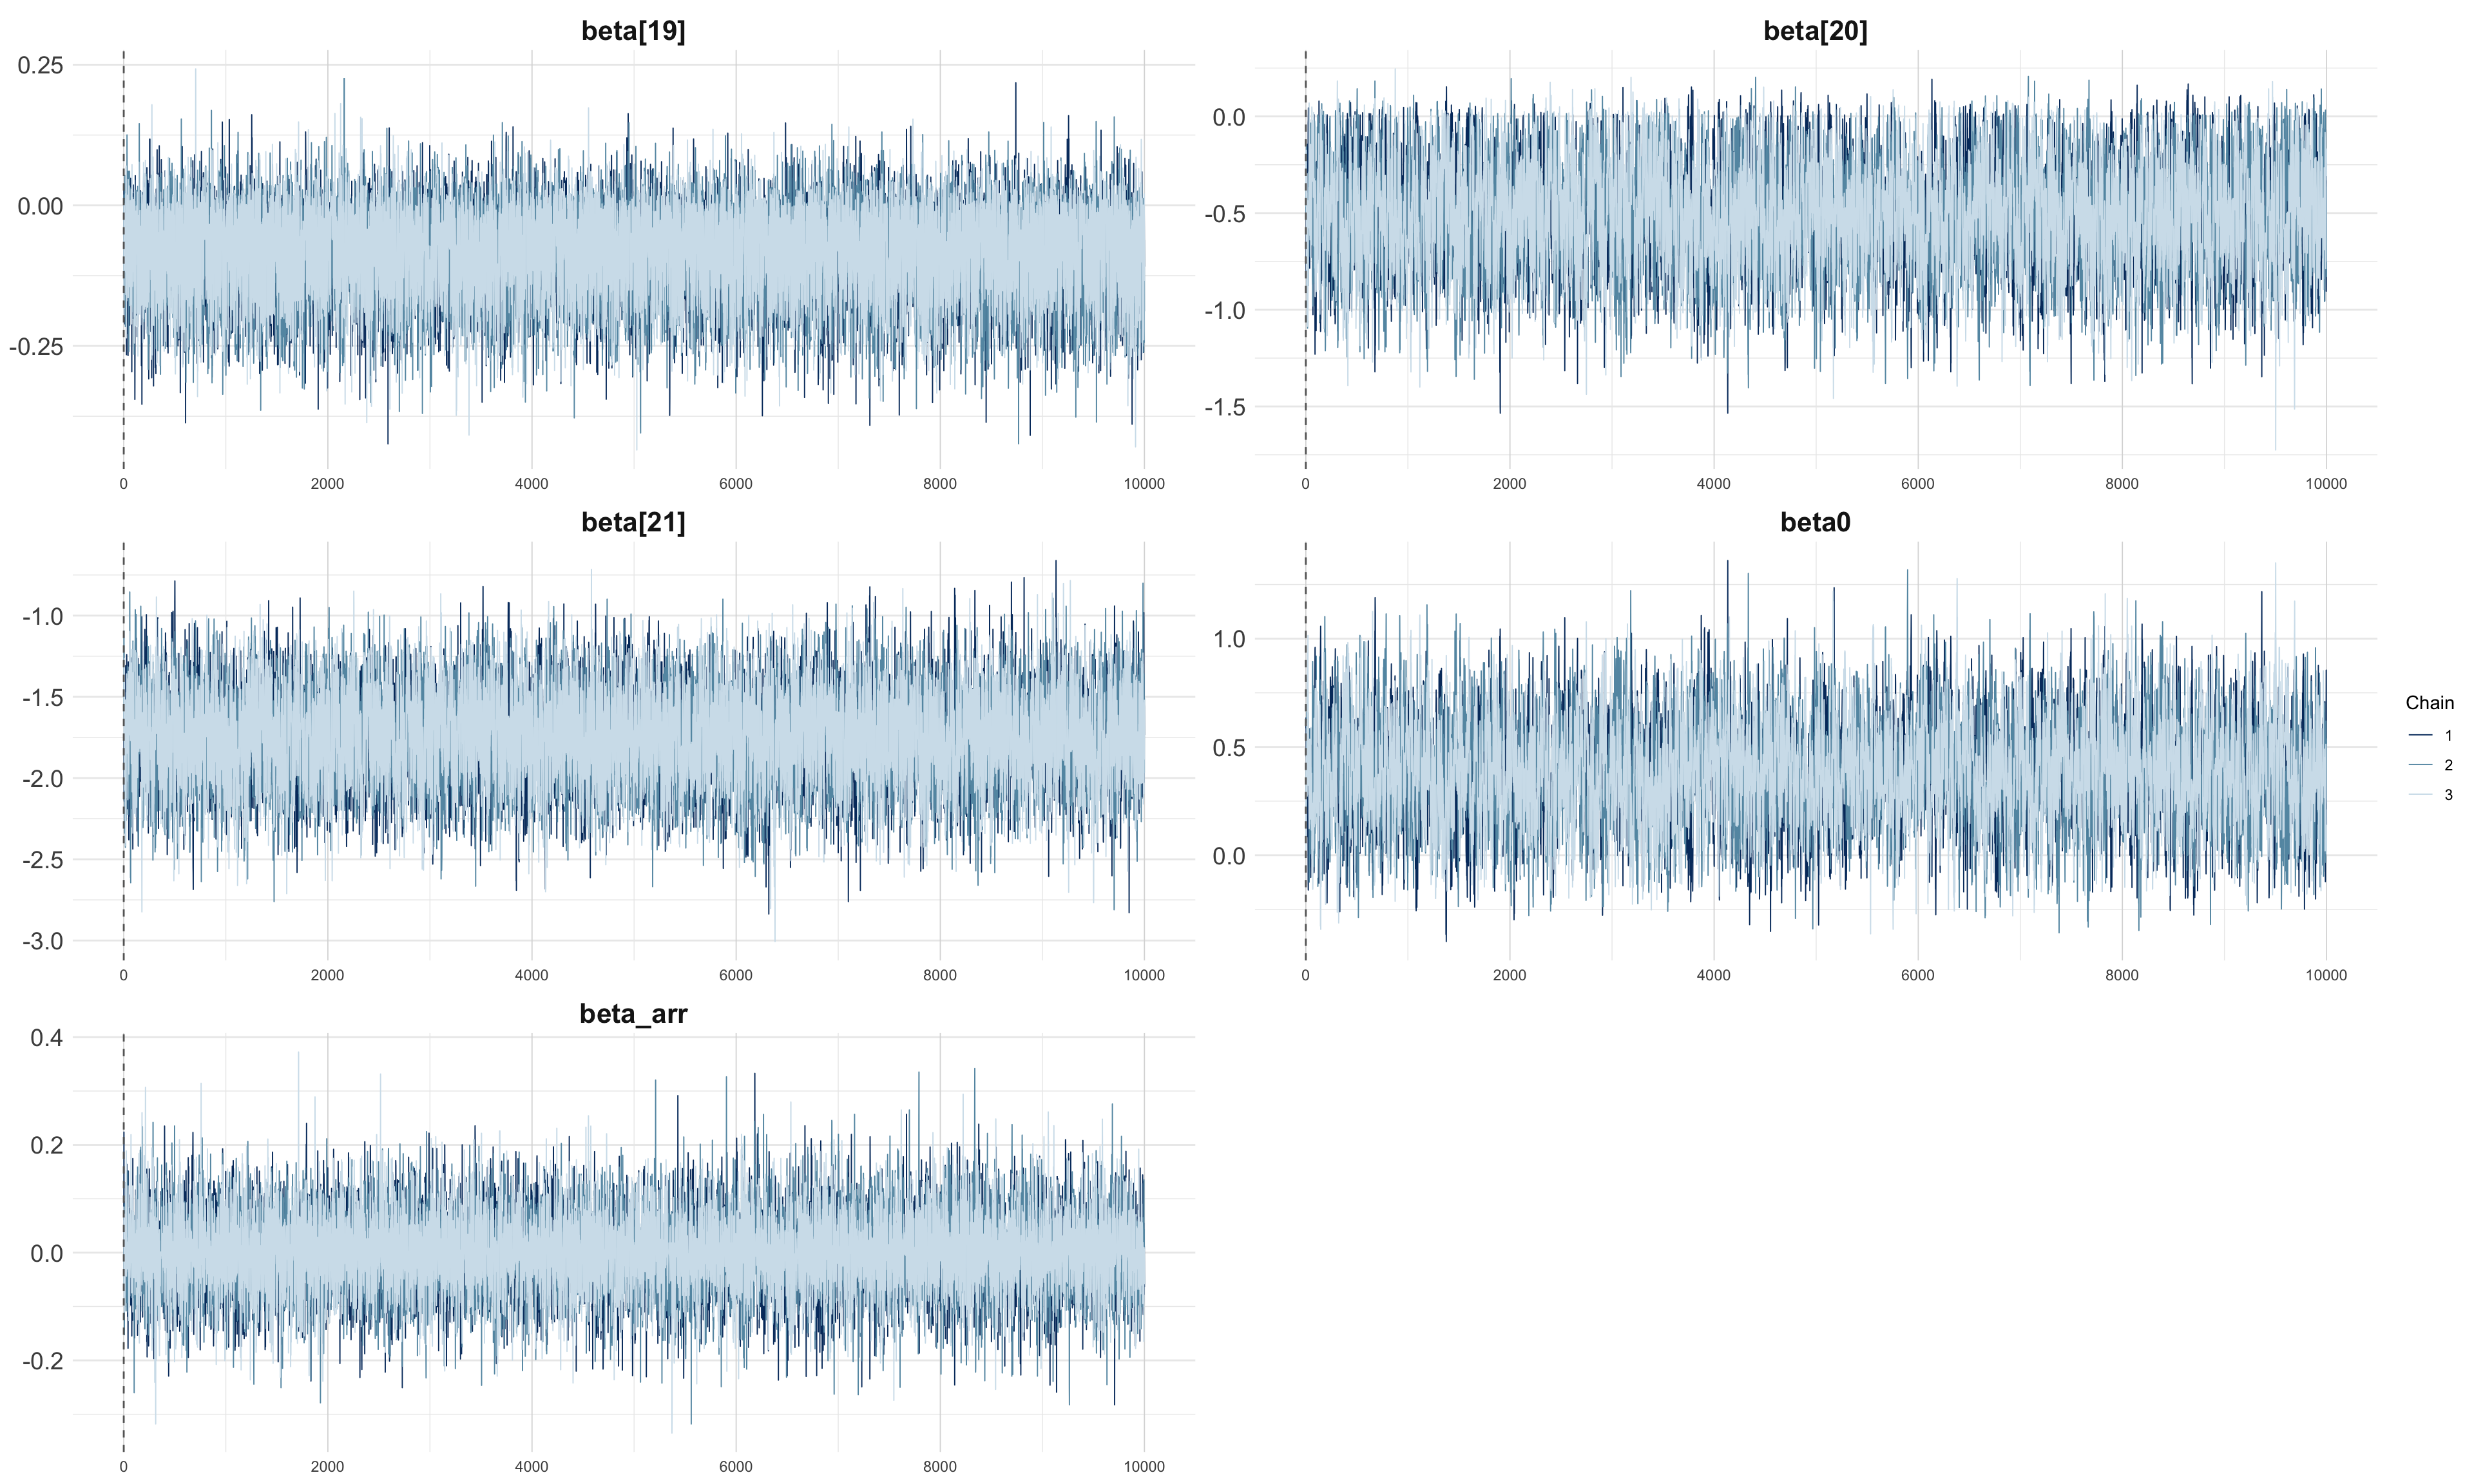
\includegraphics[width=\linewidth]{img/horseshoe_model/trace_beta_4.png}
    \caption{Group 4.}
  \end{subfigure}\hfill
  \caption{Trace plots for the remaining regression coefficients $\beta_j$, three chains.}
  \label{fig:hs_trace_beta_rest}
\end{figure}

\begin{figure}[htbp]
  \centering
  \begin{subfigure}[t]{0.48\linewidth}
    \centering
    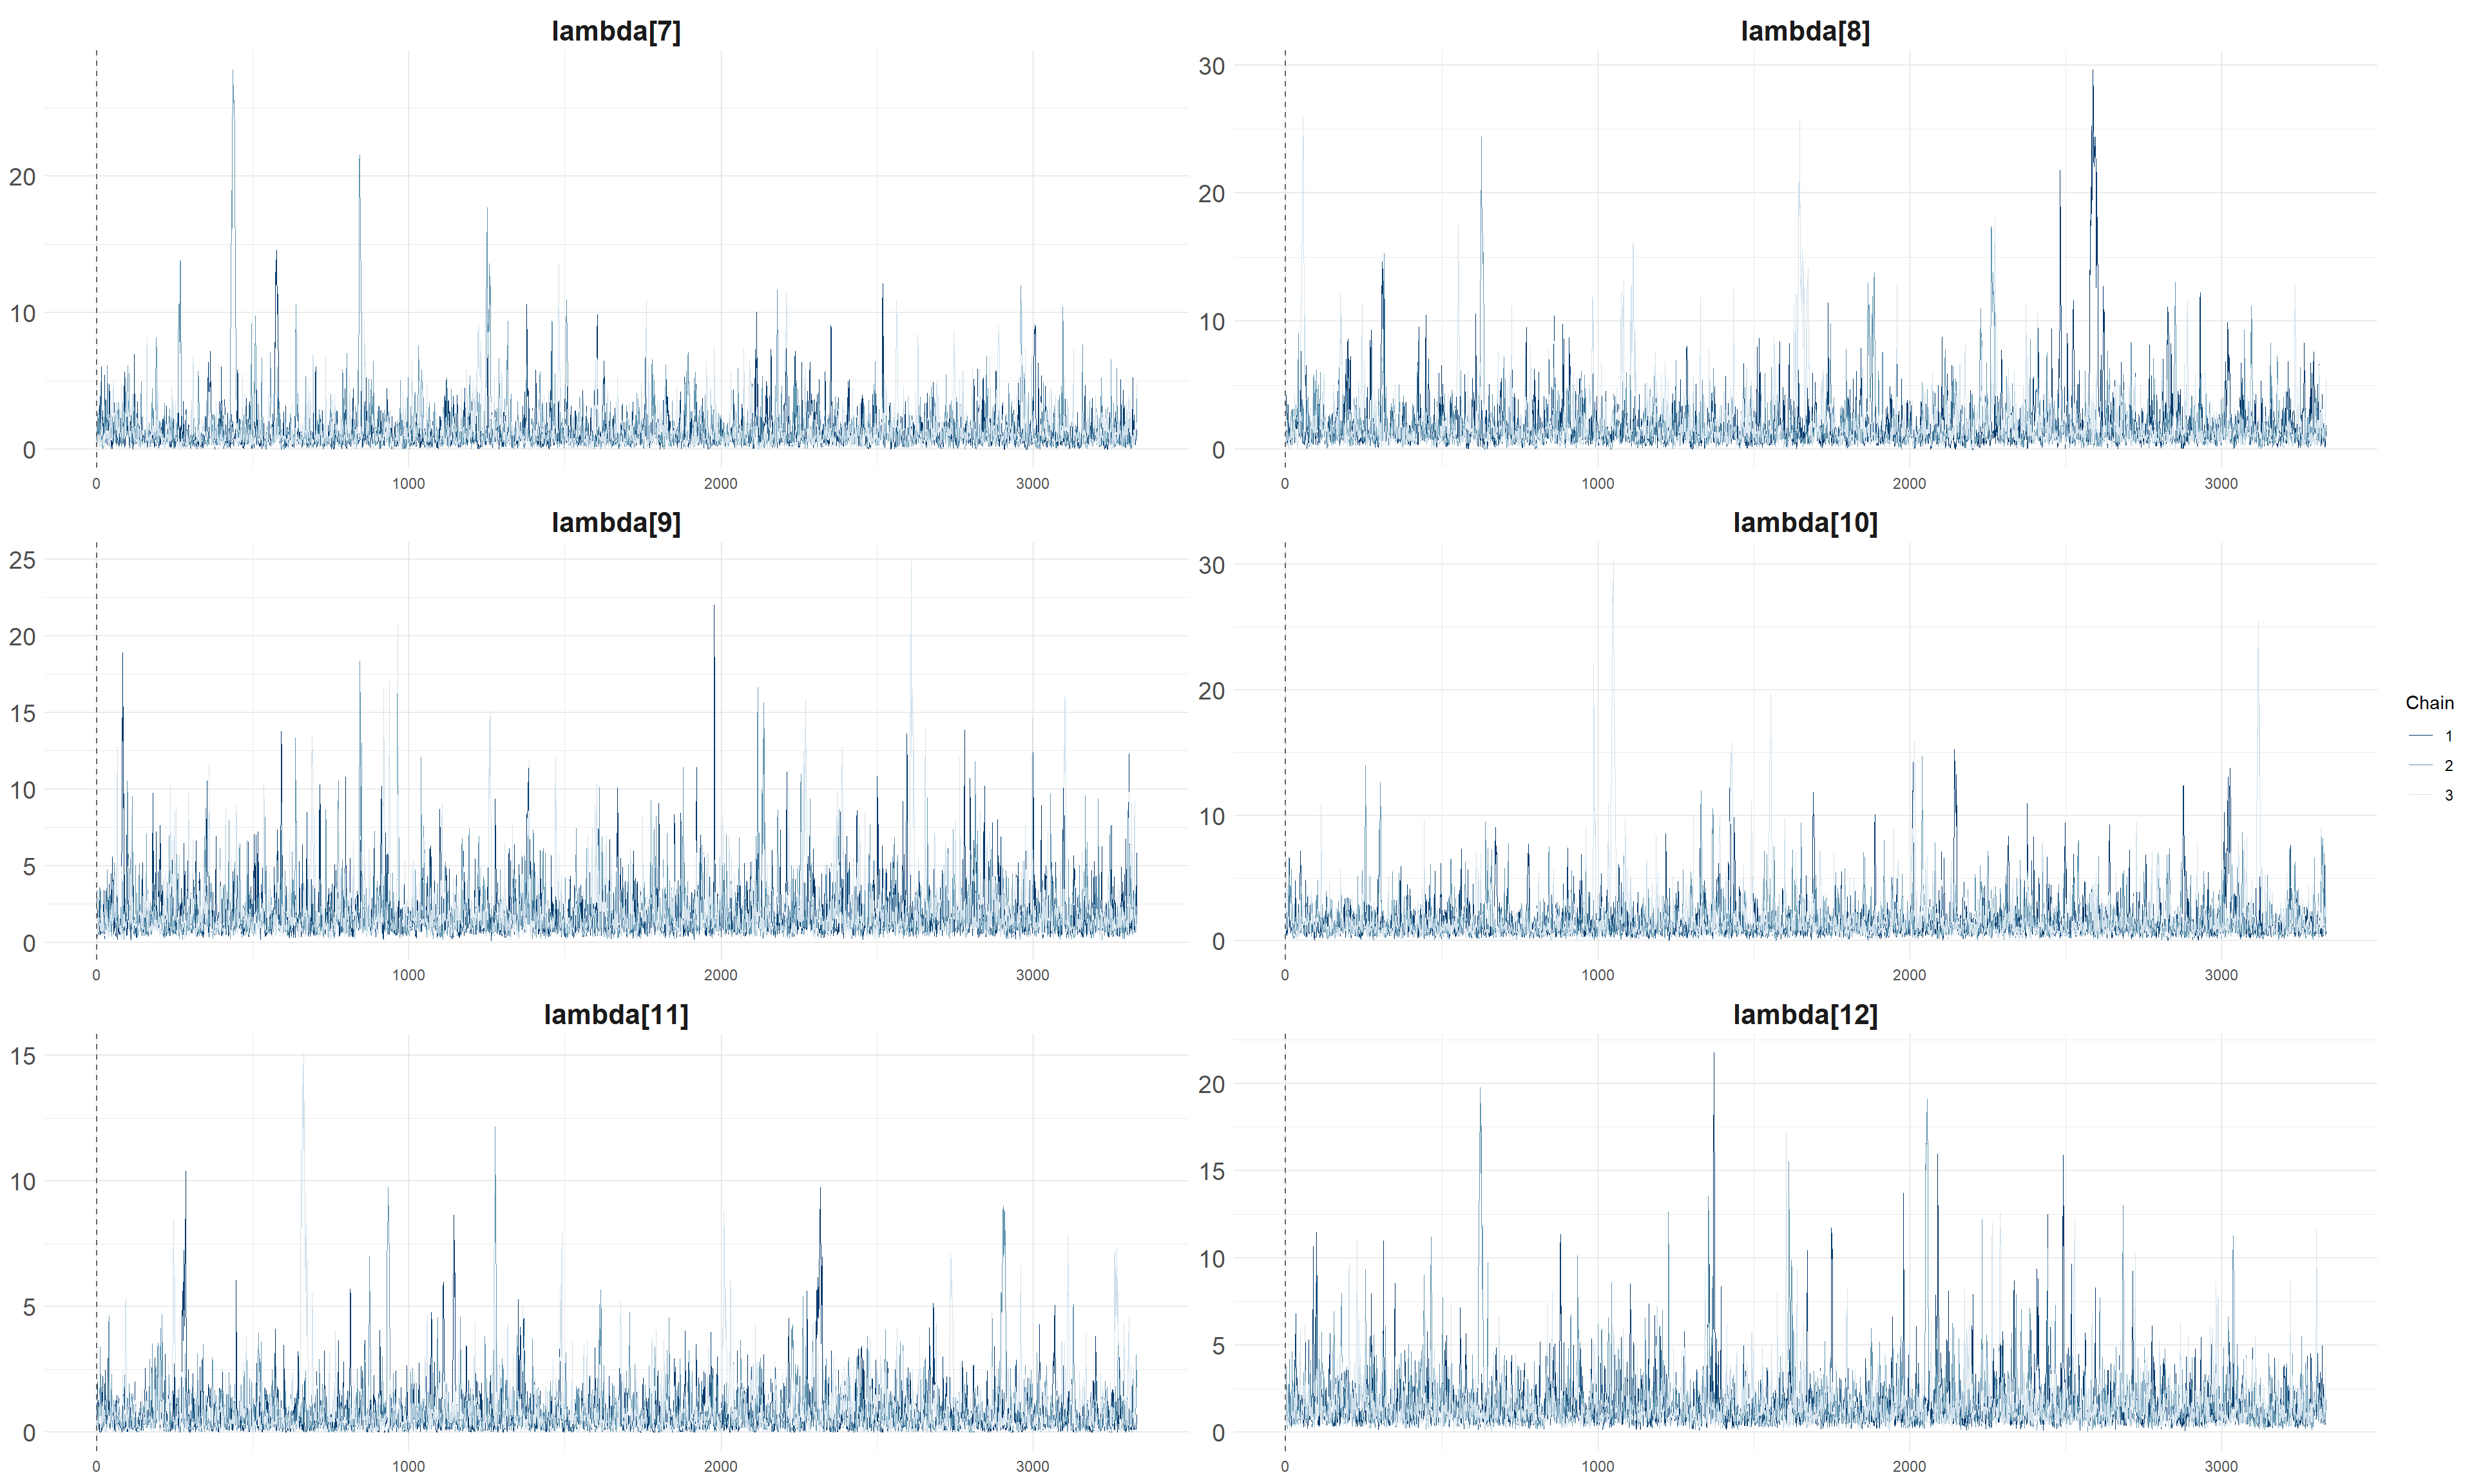
\includegraphics[width=\linewidth]{img/horseshoe_model/trace_lambda_2.png}
    \caption{Group 2.}
  \end{subfigure}\hfill
  \begin{subfigure}[t]{0.48\linewidth}
    \centering
    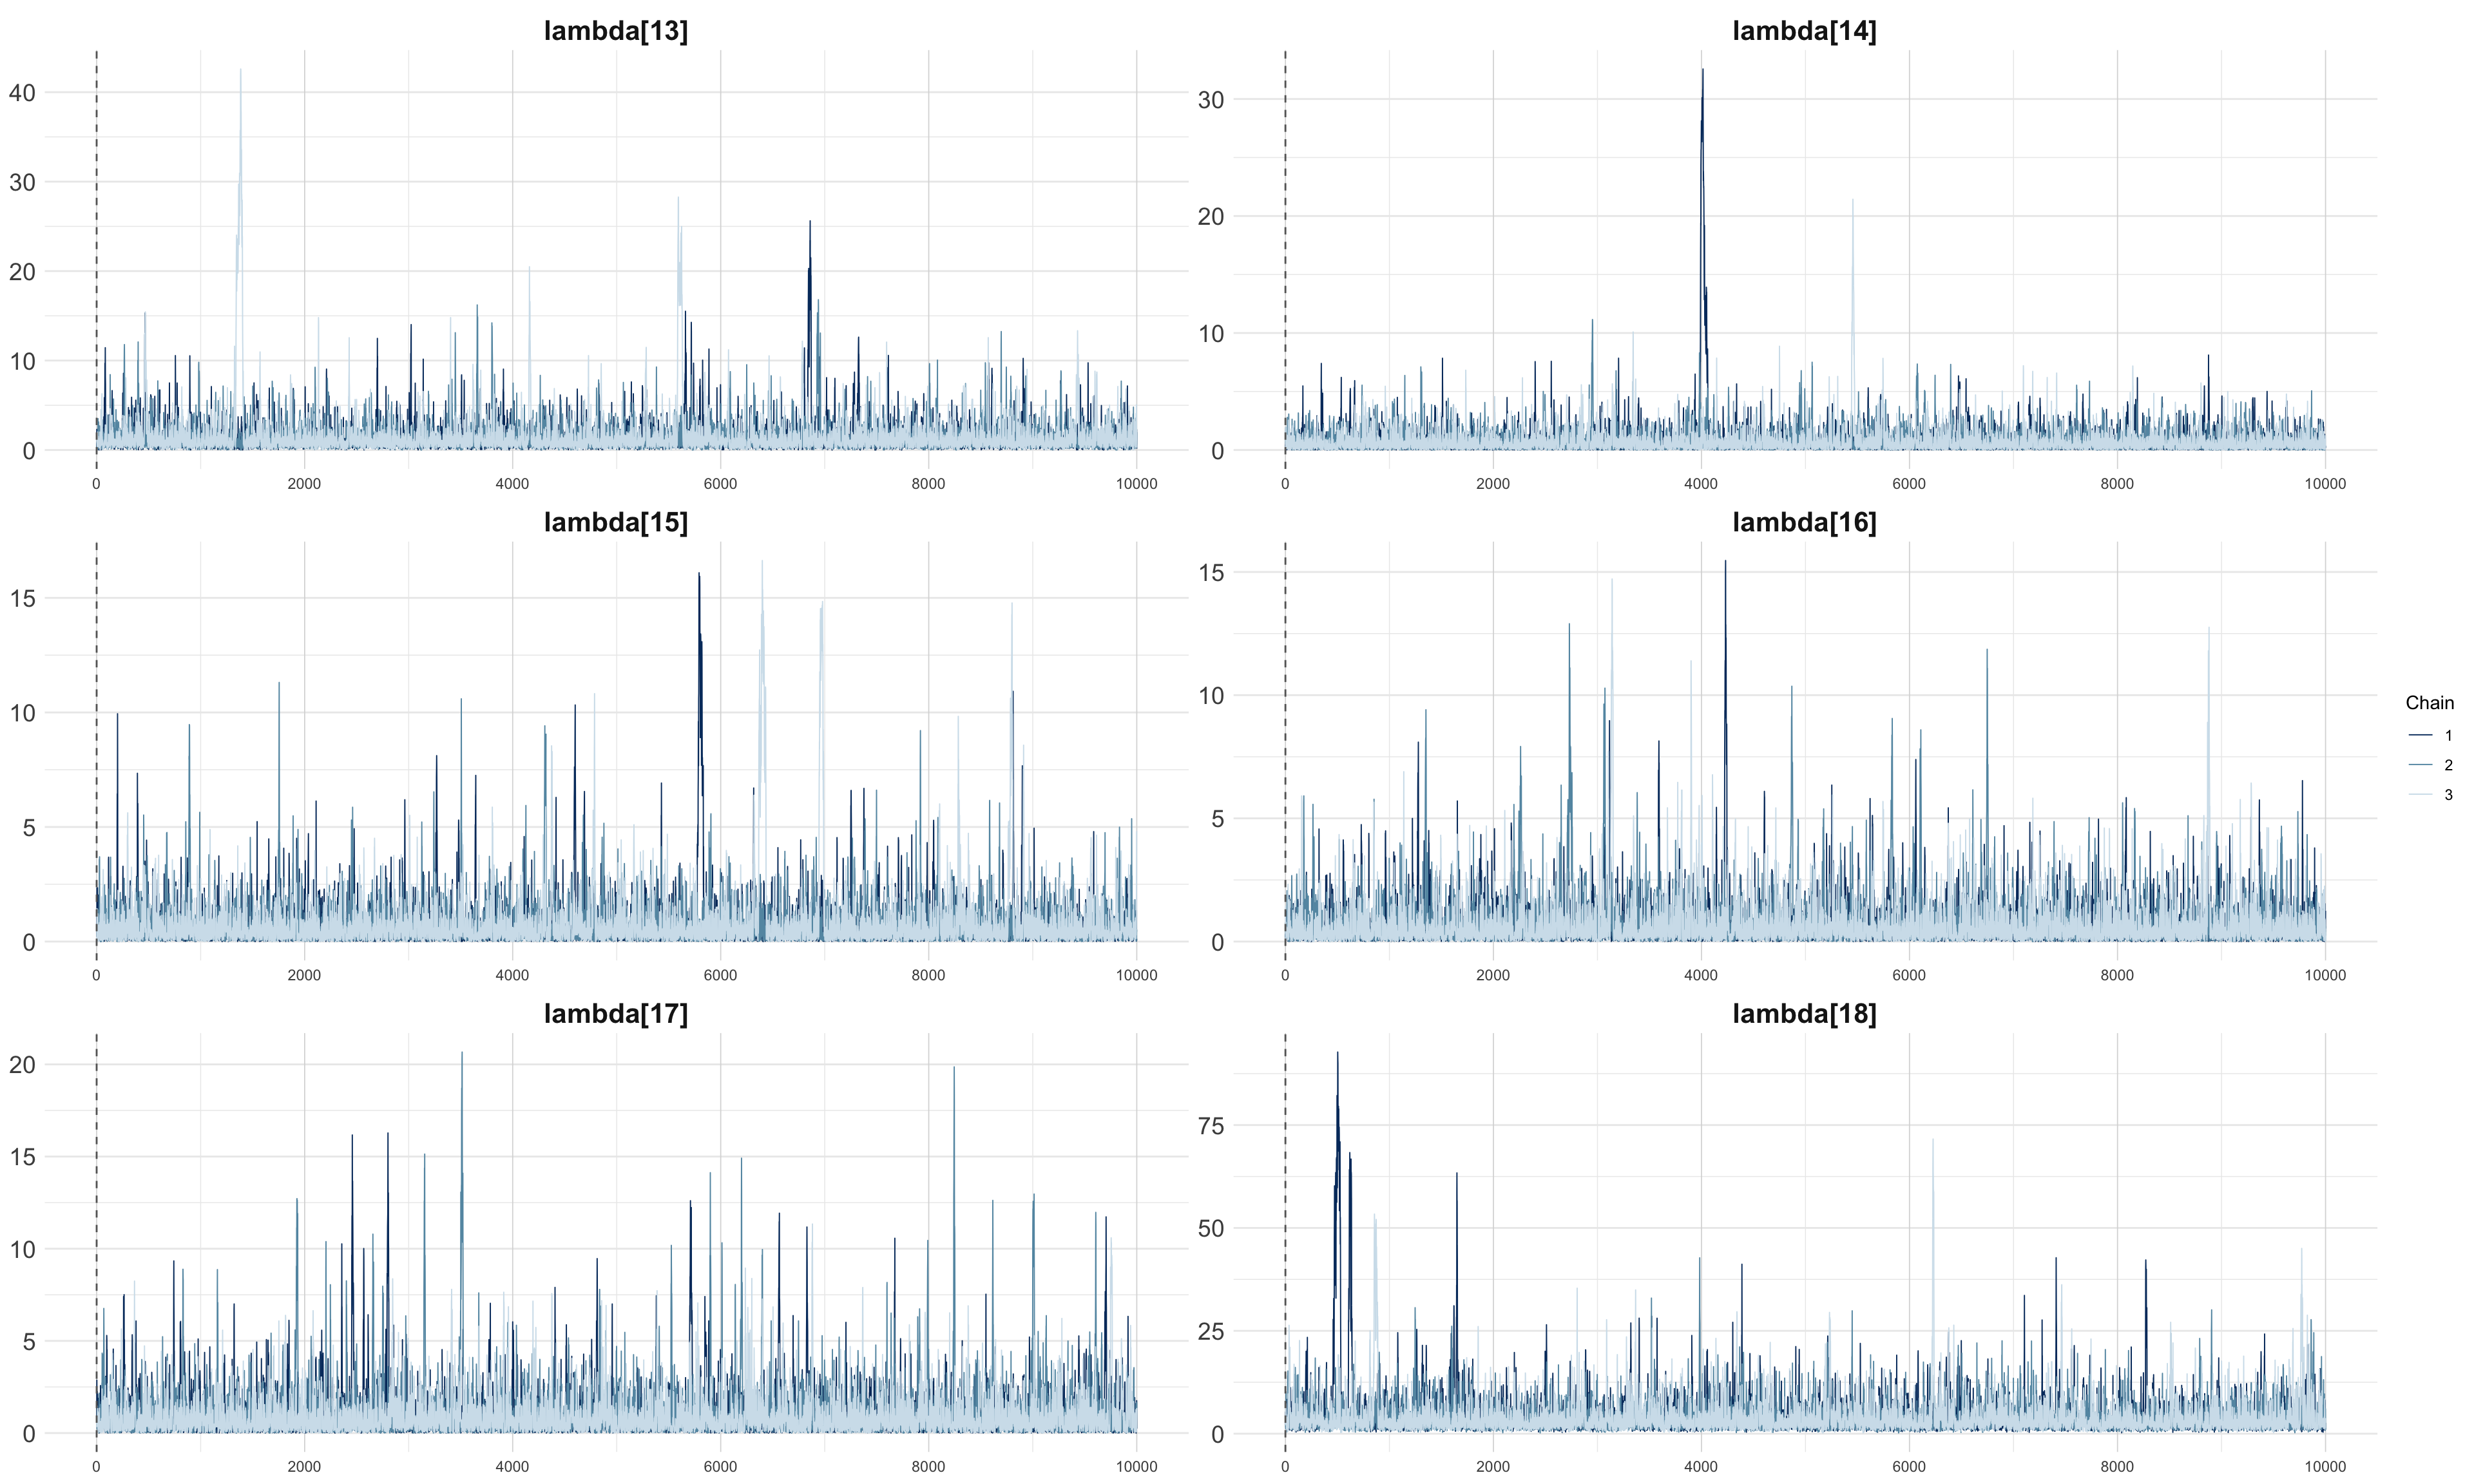
\includegraphics[width=\linewidth]{img/horseshoe_model/trace_lambda_3.png}
    \caption{Group 3.}
  \end{subfigure}\hfill
  \begin{subfigure}[t]{0.48\linewidth}
    \centering
    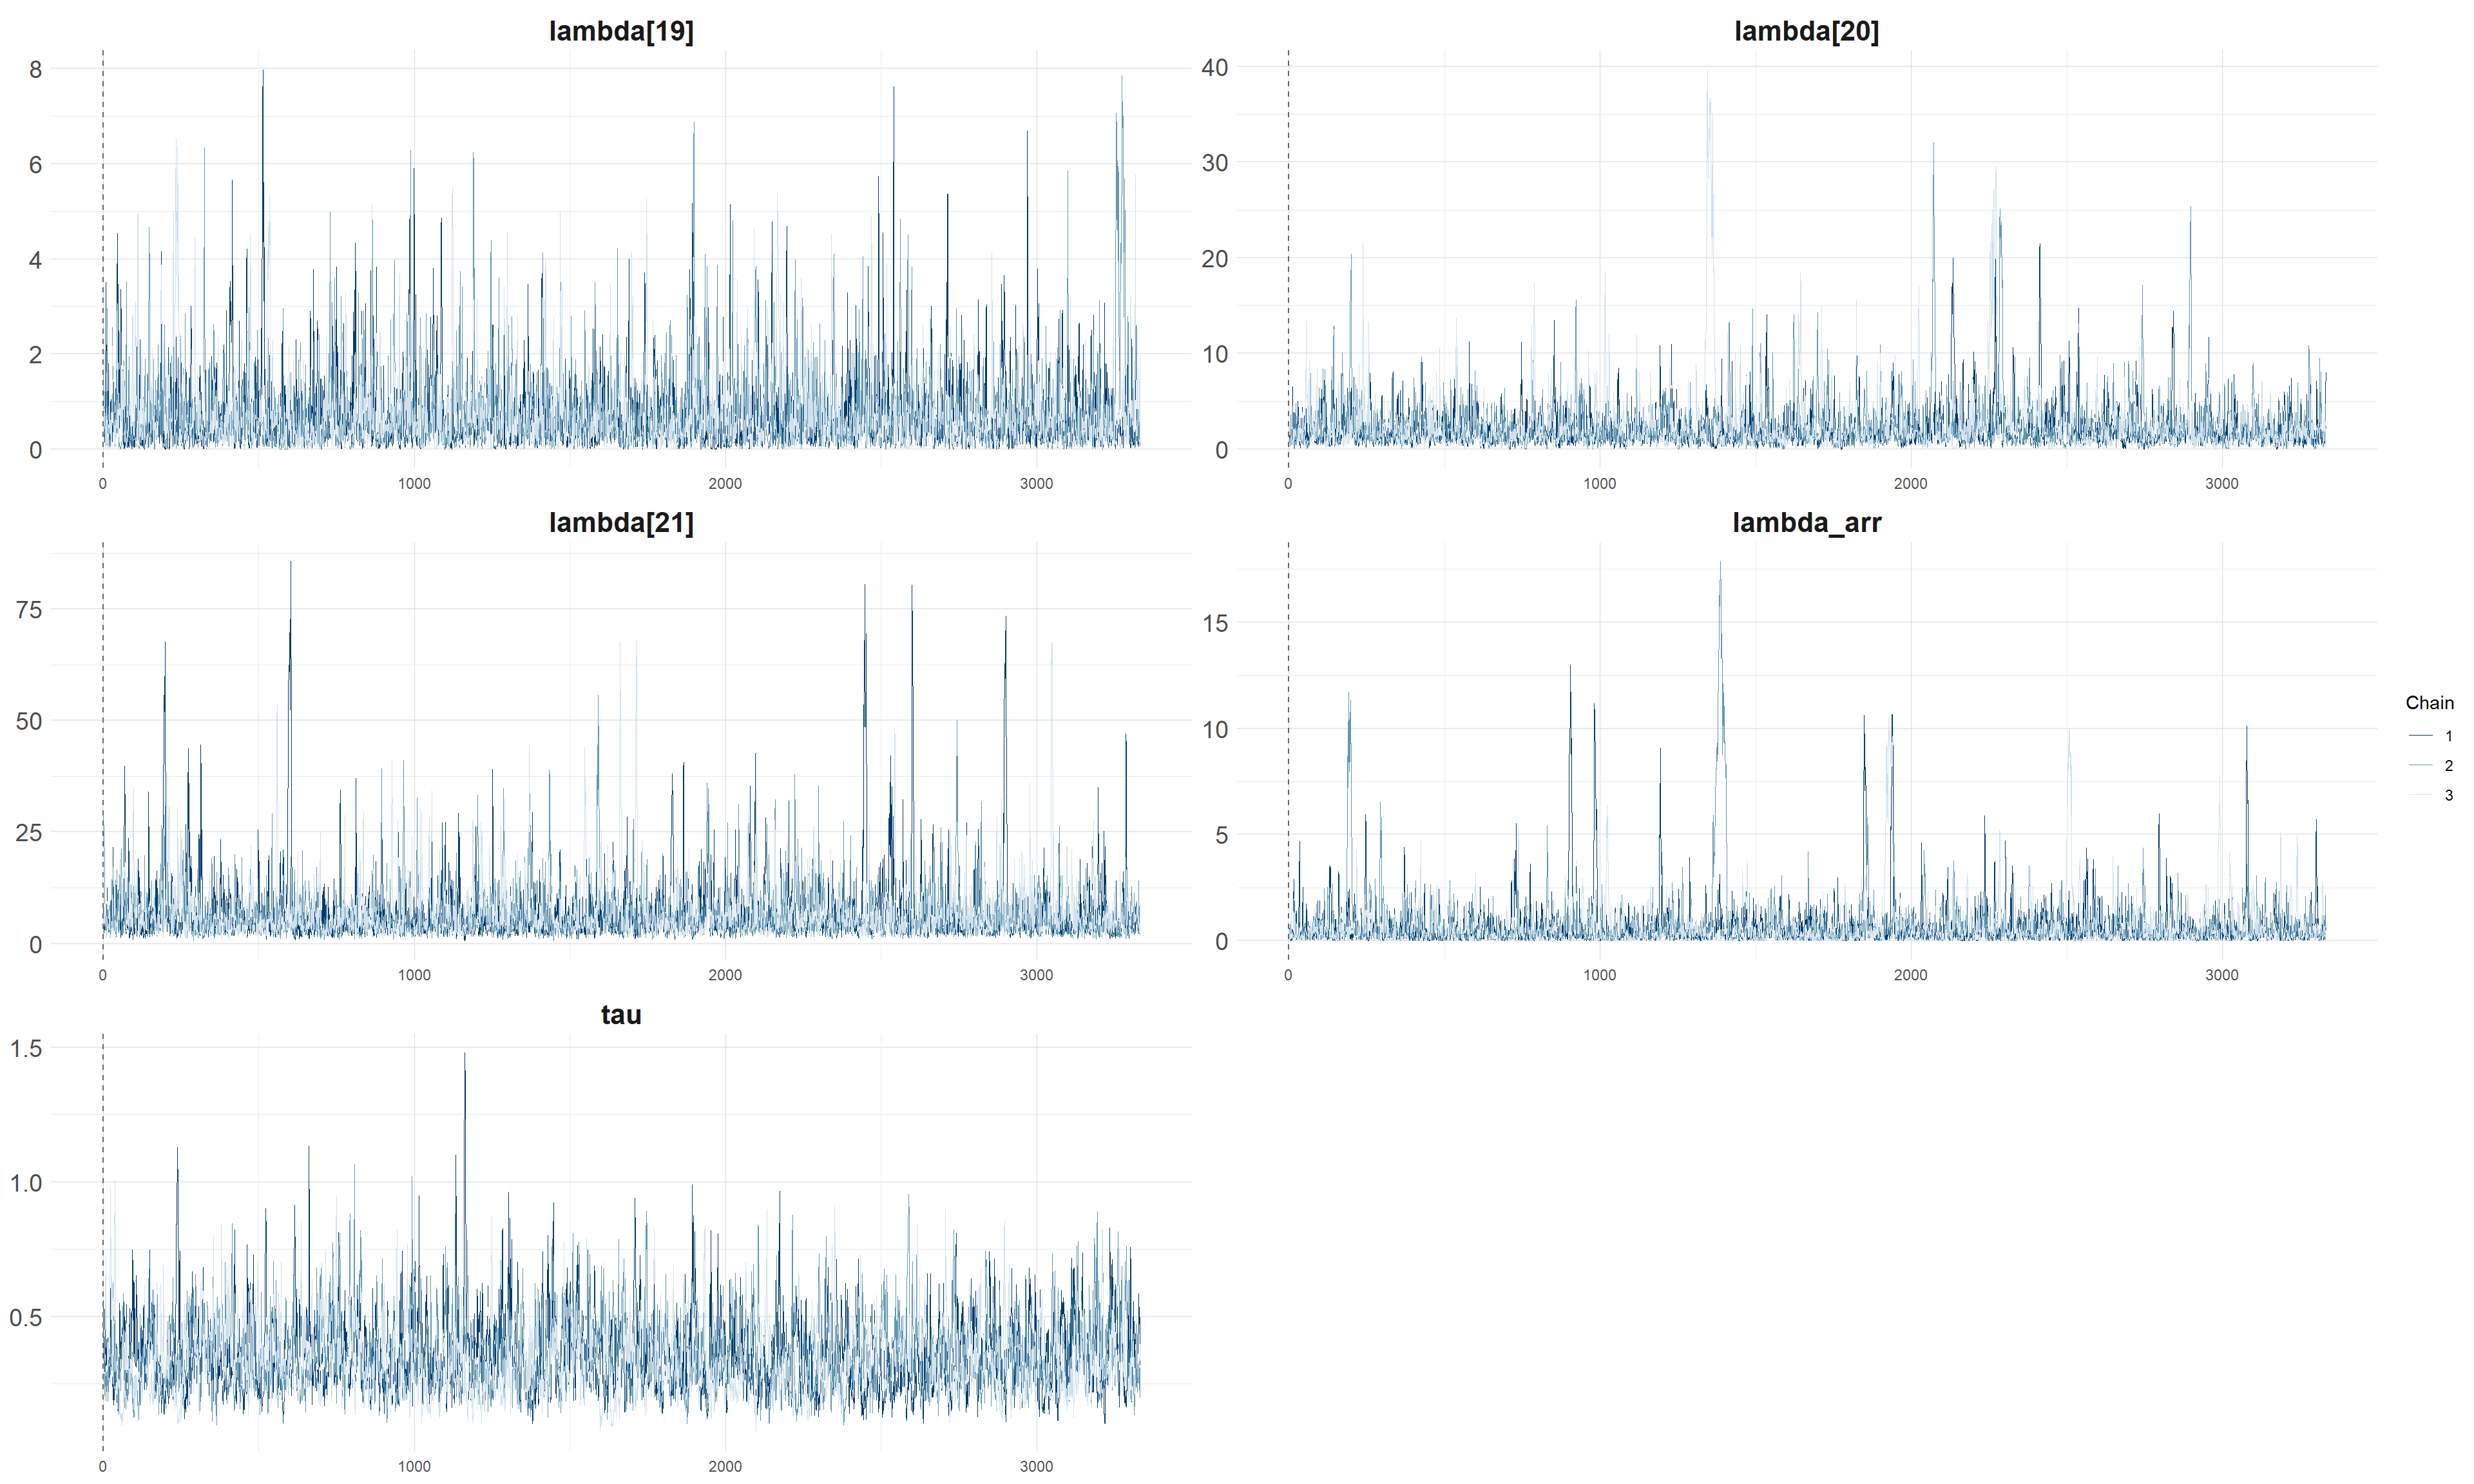
\includegraphics[width=\linewidth]{img/horseshoe_model/trace_lambda_4.png}
    \caption{Group 4.}
  \end{subfigure}\hfill
  \caption{Trace plots for the remaining scale parameters $\lambda_j$, three chains.}
  \label{fig:hs_trace_lambda_rest}
\end{figure}

\subsection*{Autocorrelation}
Autocorrelation functions for every parameter, one set per chain. The
coefficients decay within a few lags; the local scales decay more slowly, which
is the expected behaviour for a horseshoe and the reason for the thinning.
\begin{figure}[htbp]
  \centering
  \begin{subfigure}[t]{0.48\linewidth}
    \centering
    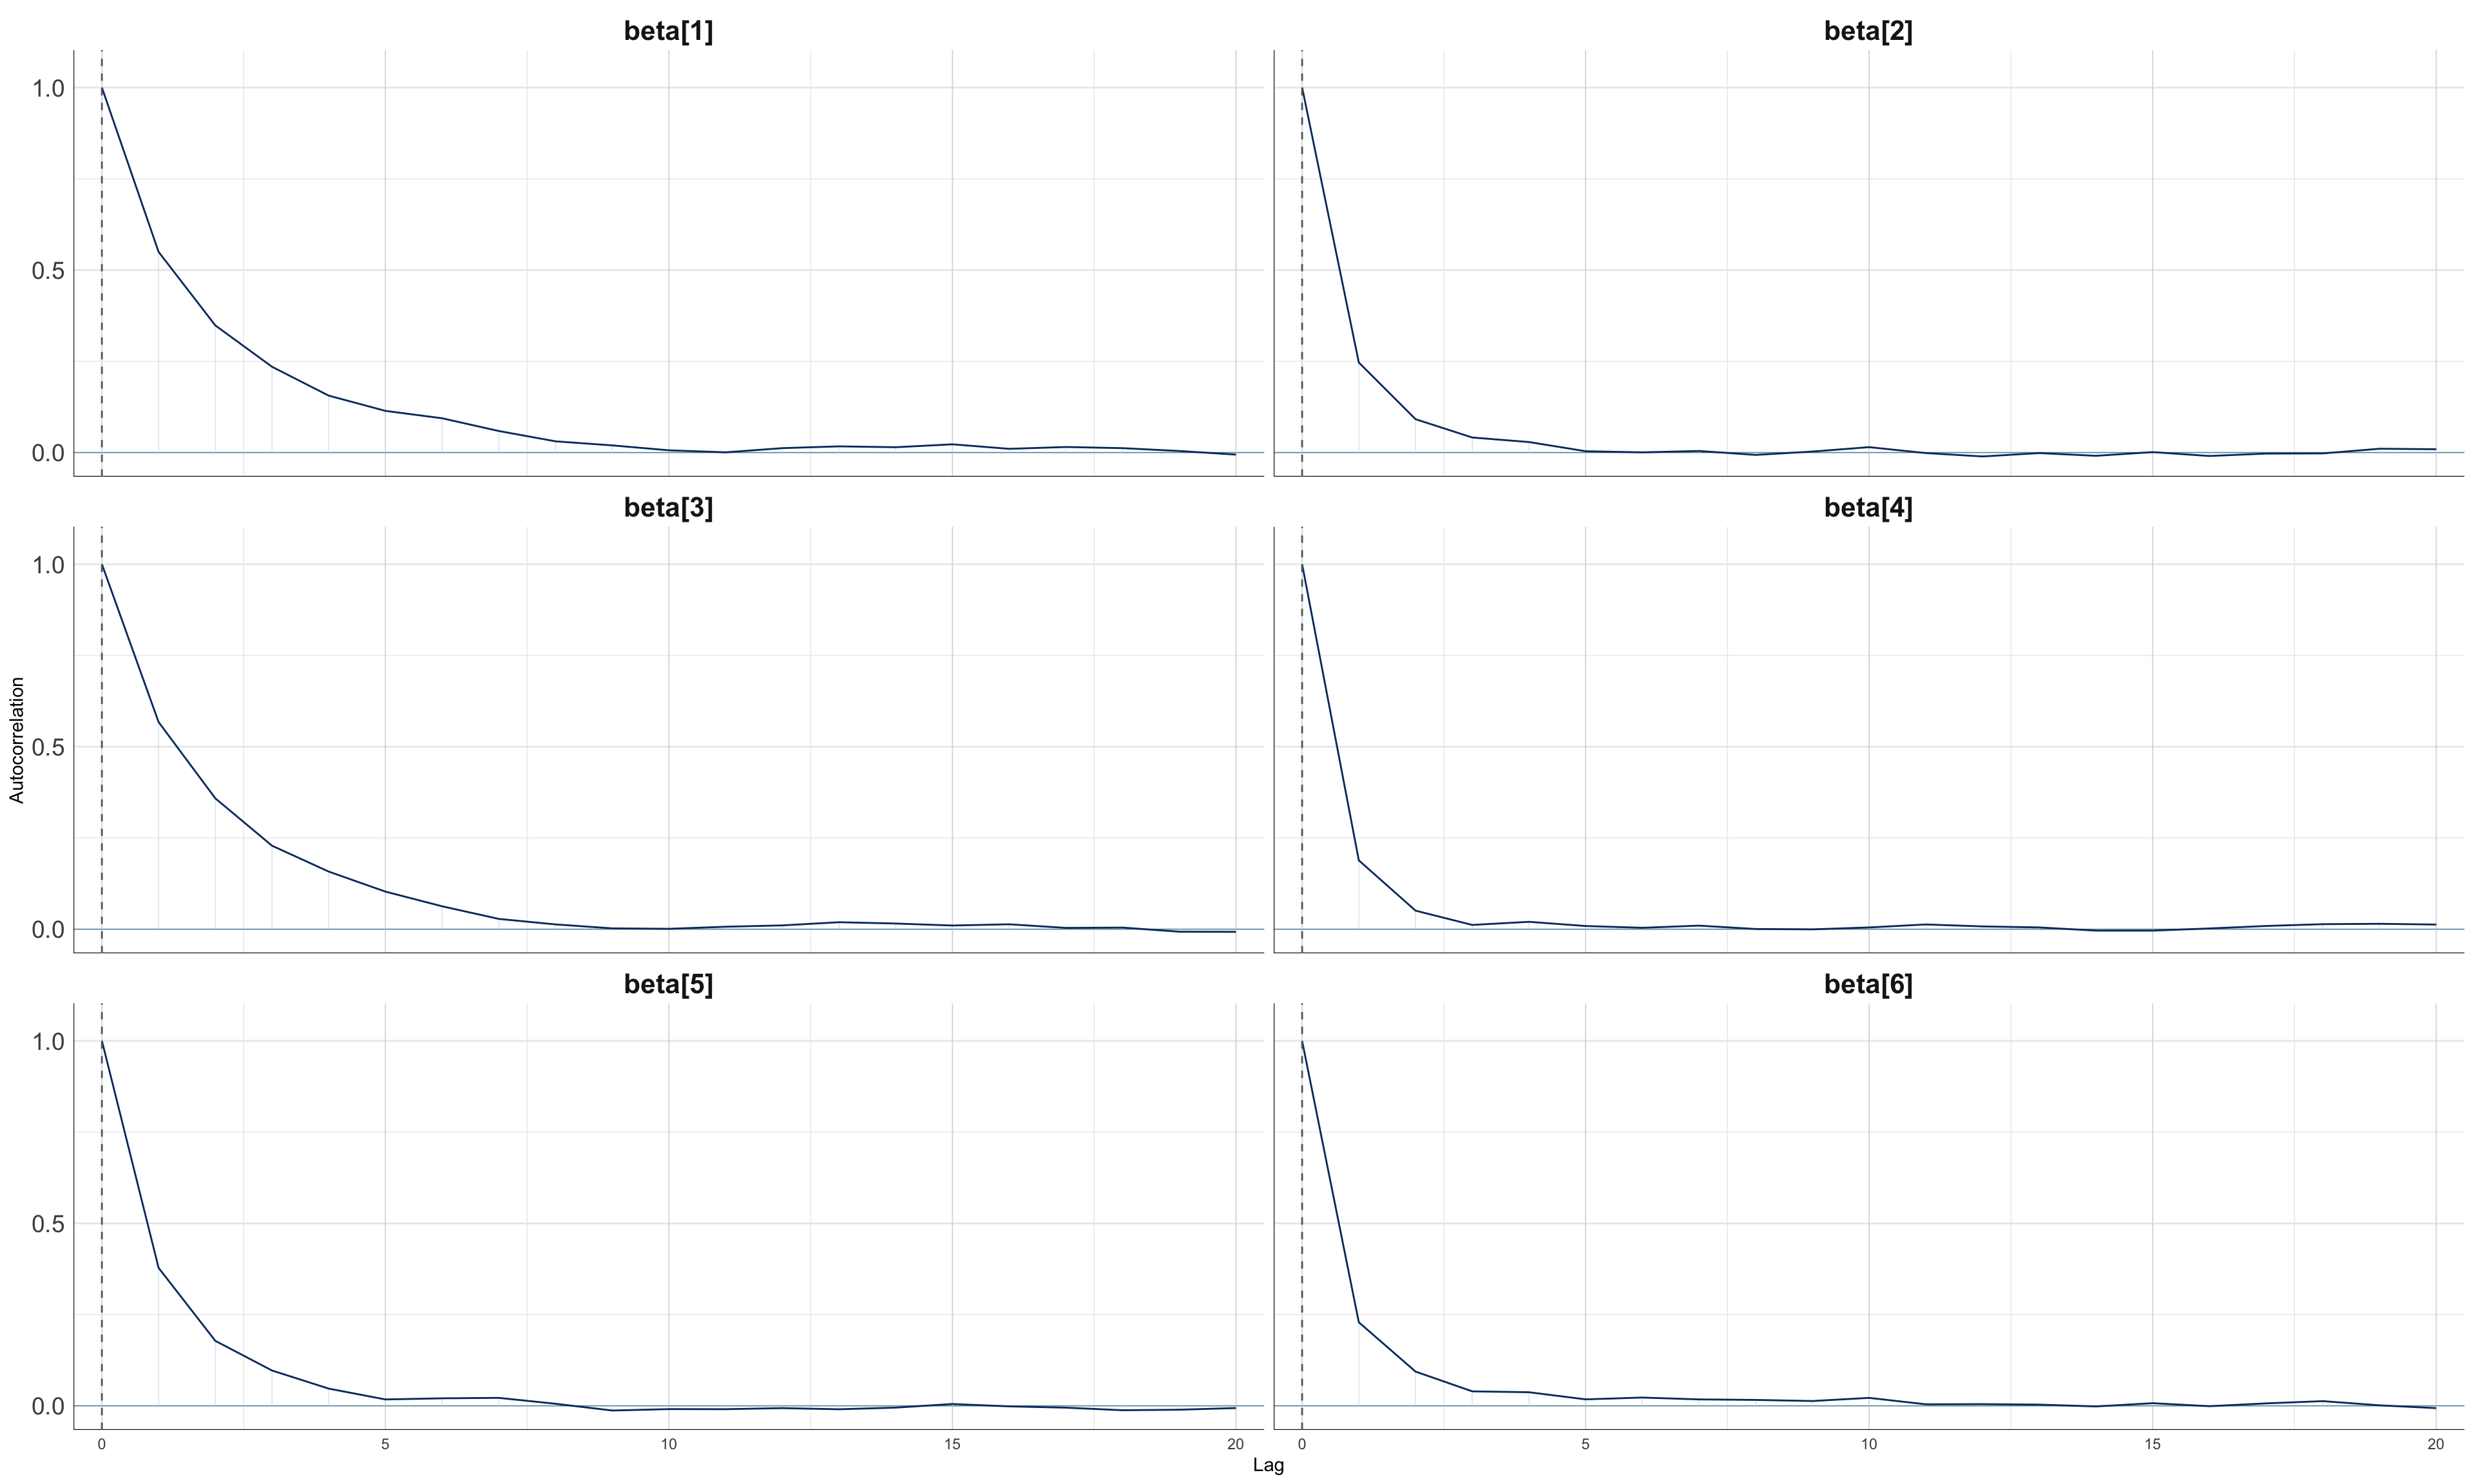
\includegraphics[width=\linewidth]{img/horseshoe_model/acf_beta_chain1_1.png}
    \caption{Group 1.}
  \end{subfigure}\hfill
  \begin{subfigure}[t]{0.48\linewidth}
    \centering
    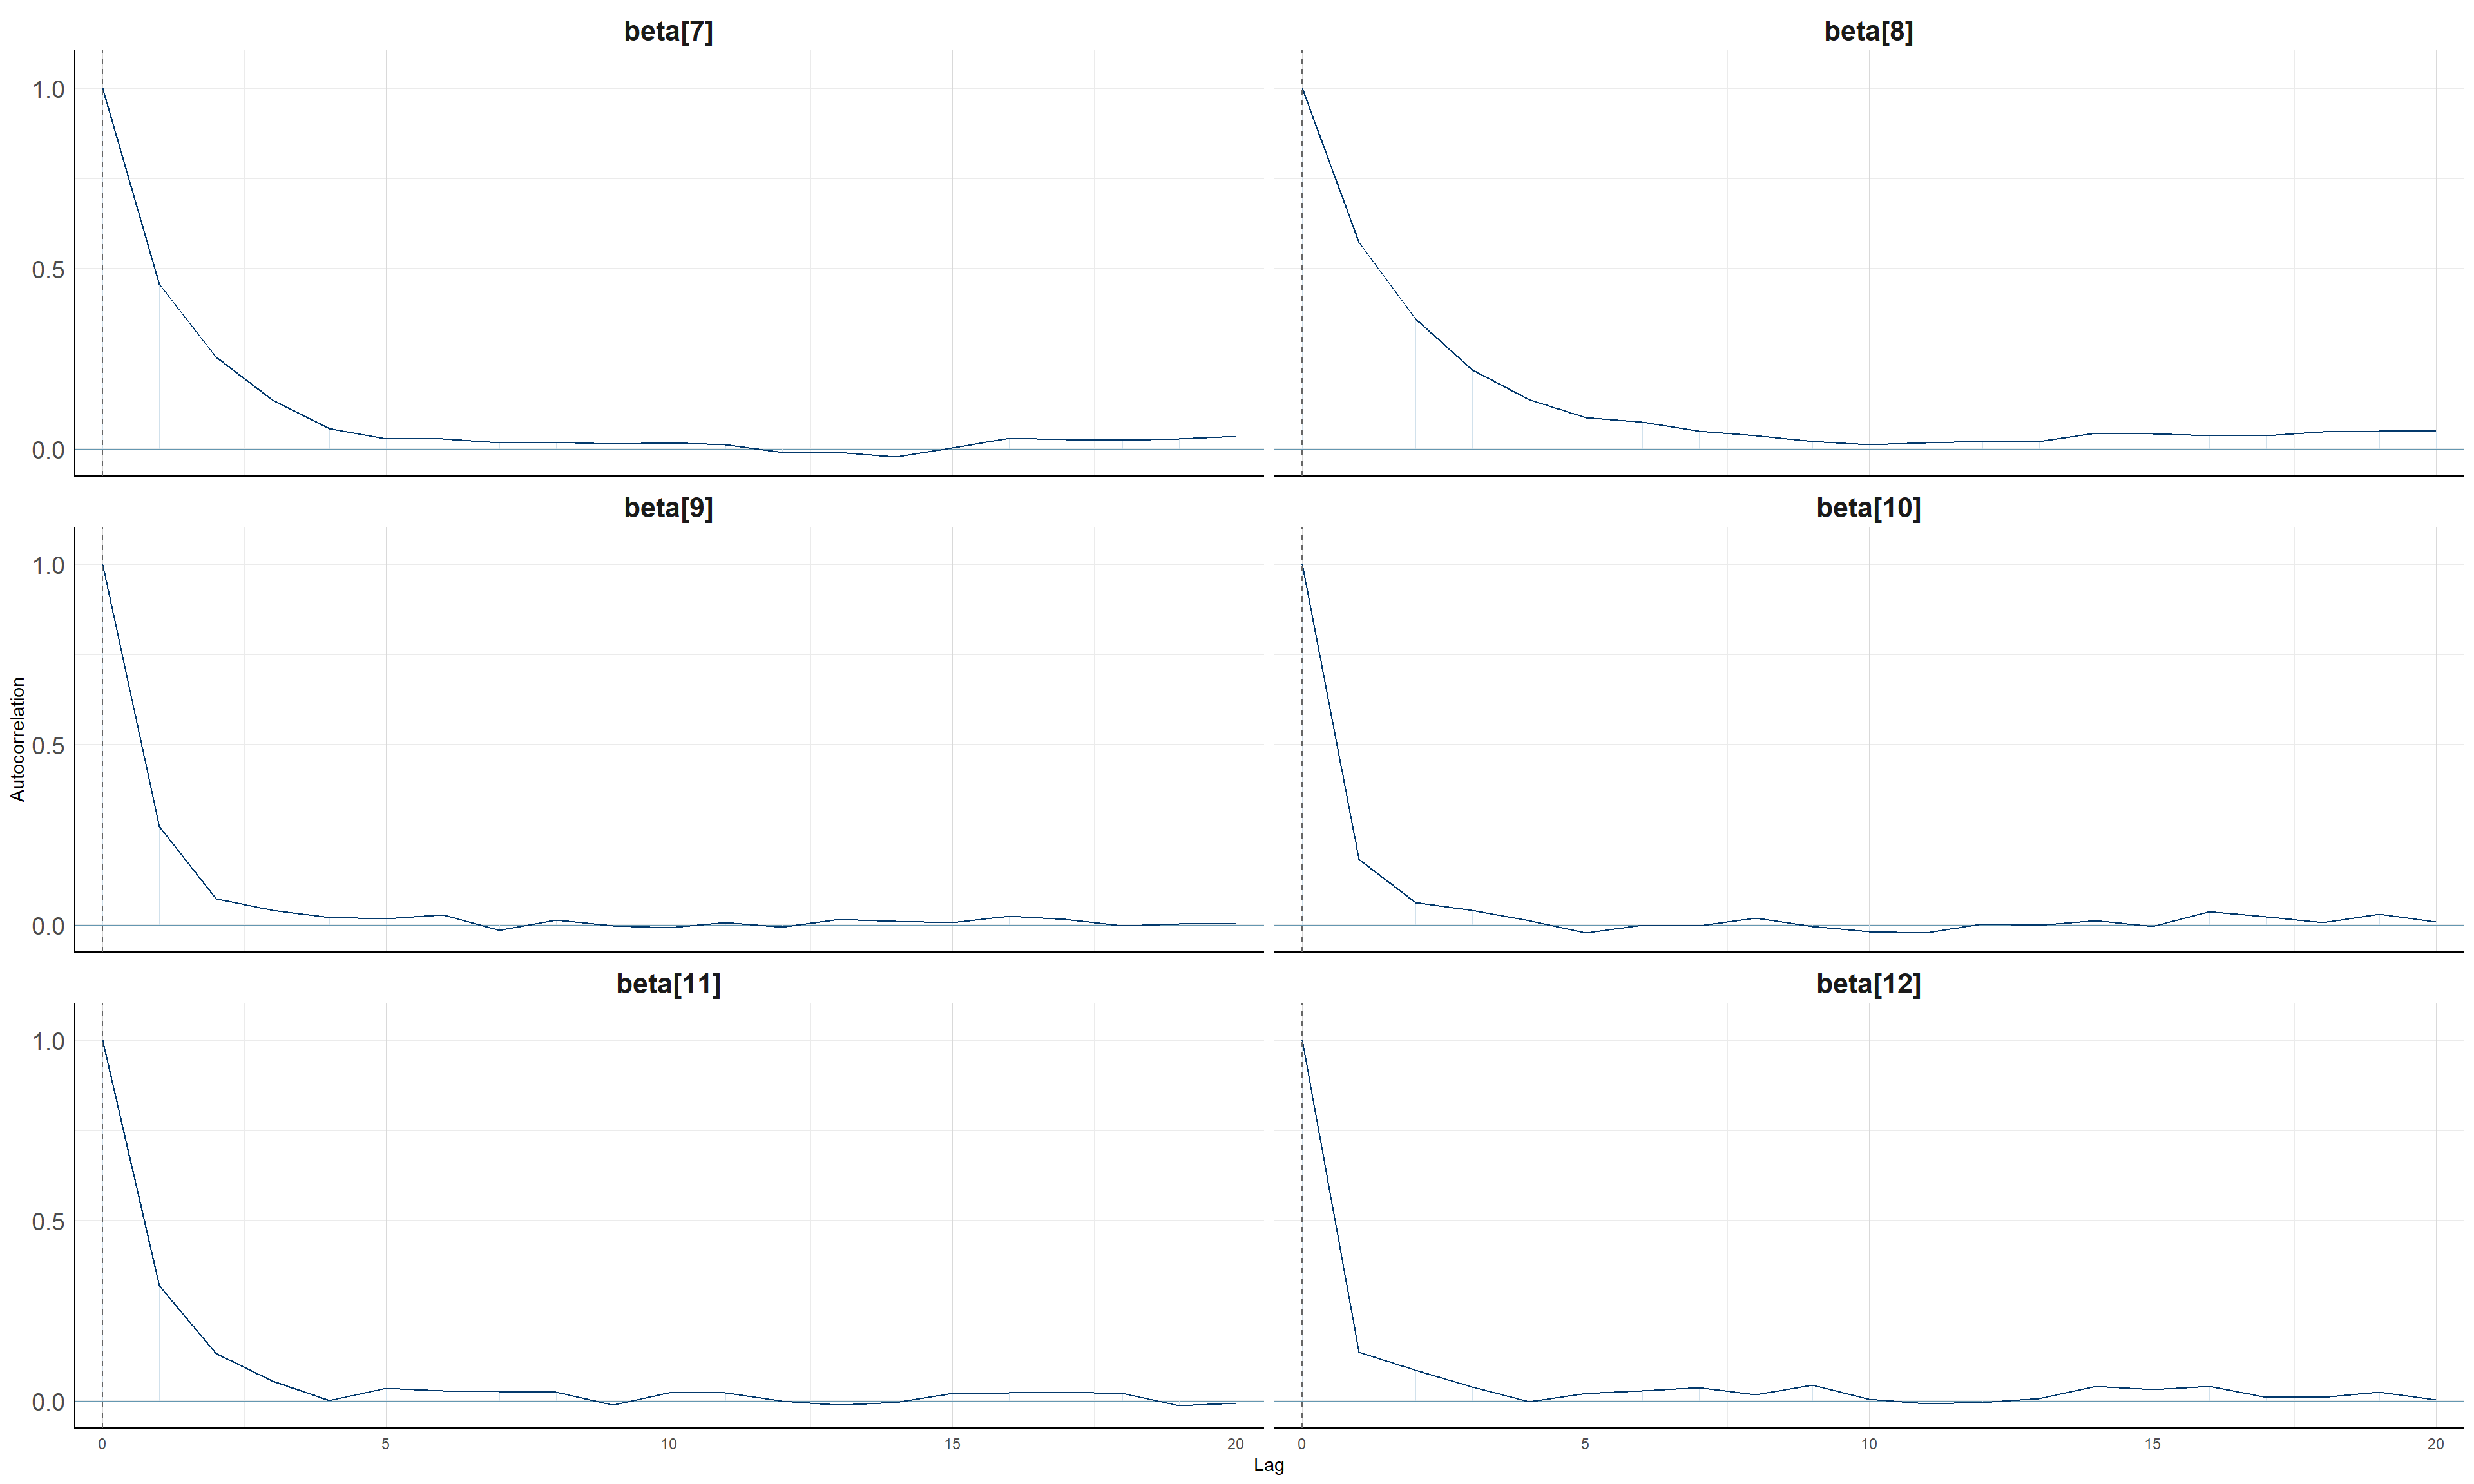
\includegraphics[width=\linewidth]{img/horseshoe_model/acf_beta_chain1_2.png}
    \caption{Group 2.}
  \end{subfigure}\hfill
  \begin{subfigure}[t]{0.48\linewidth}
    \centering
    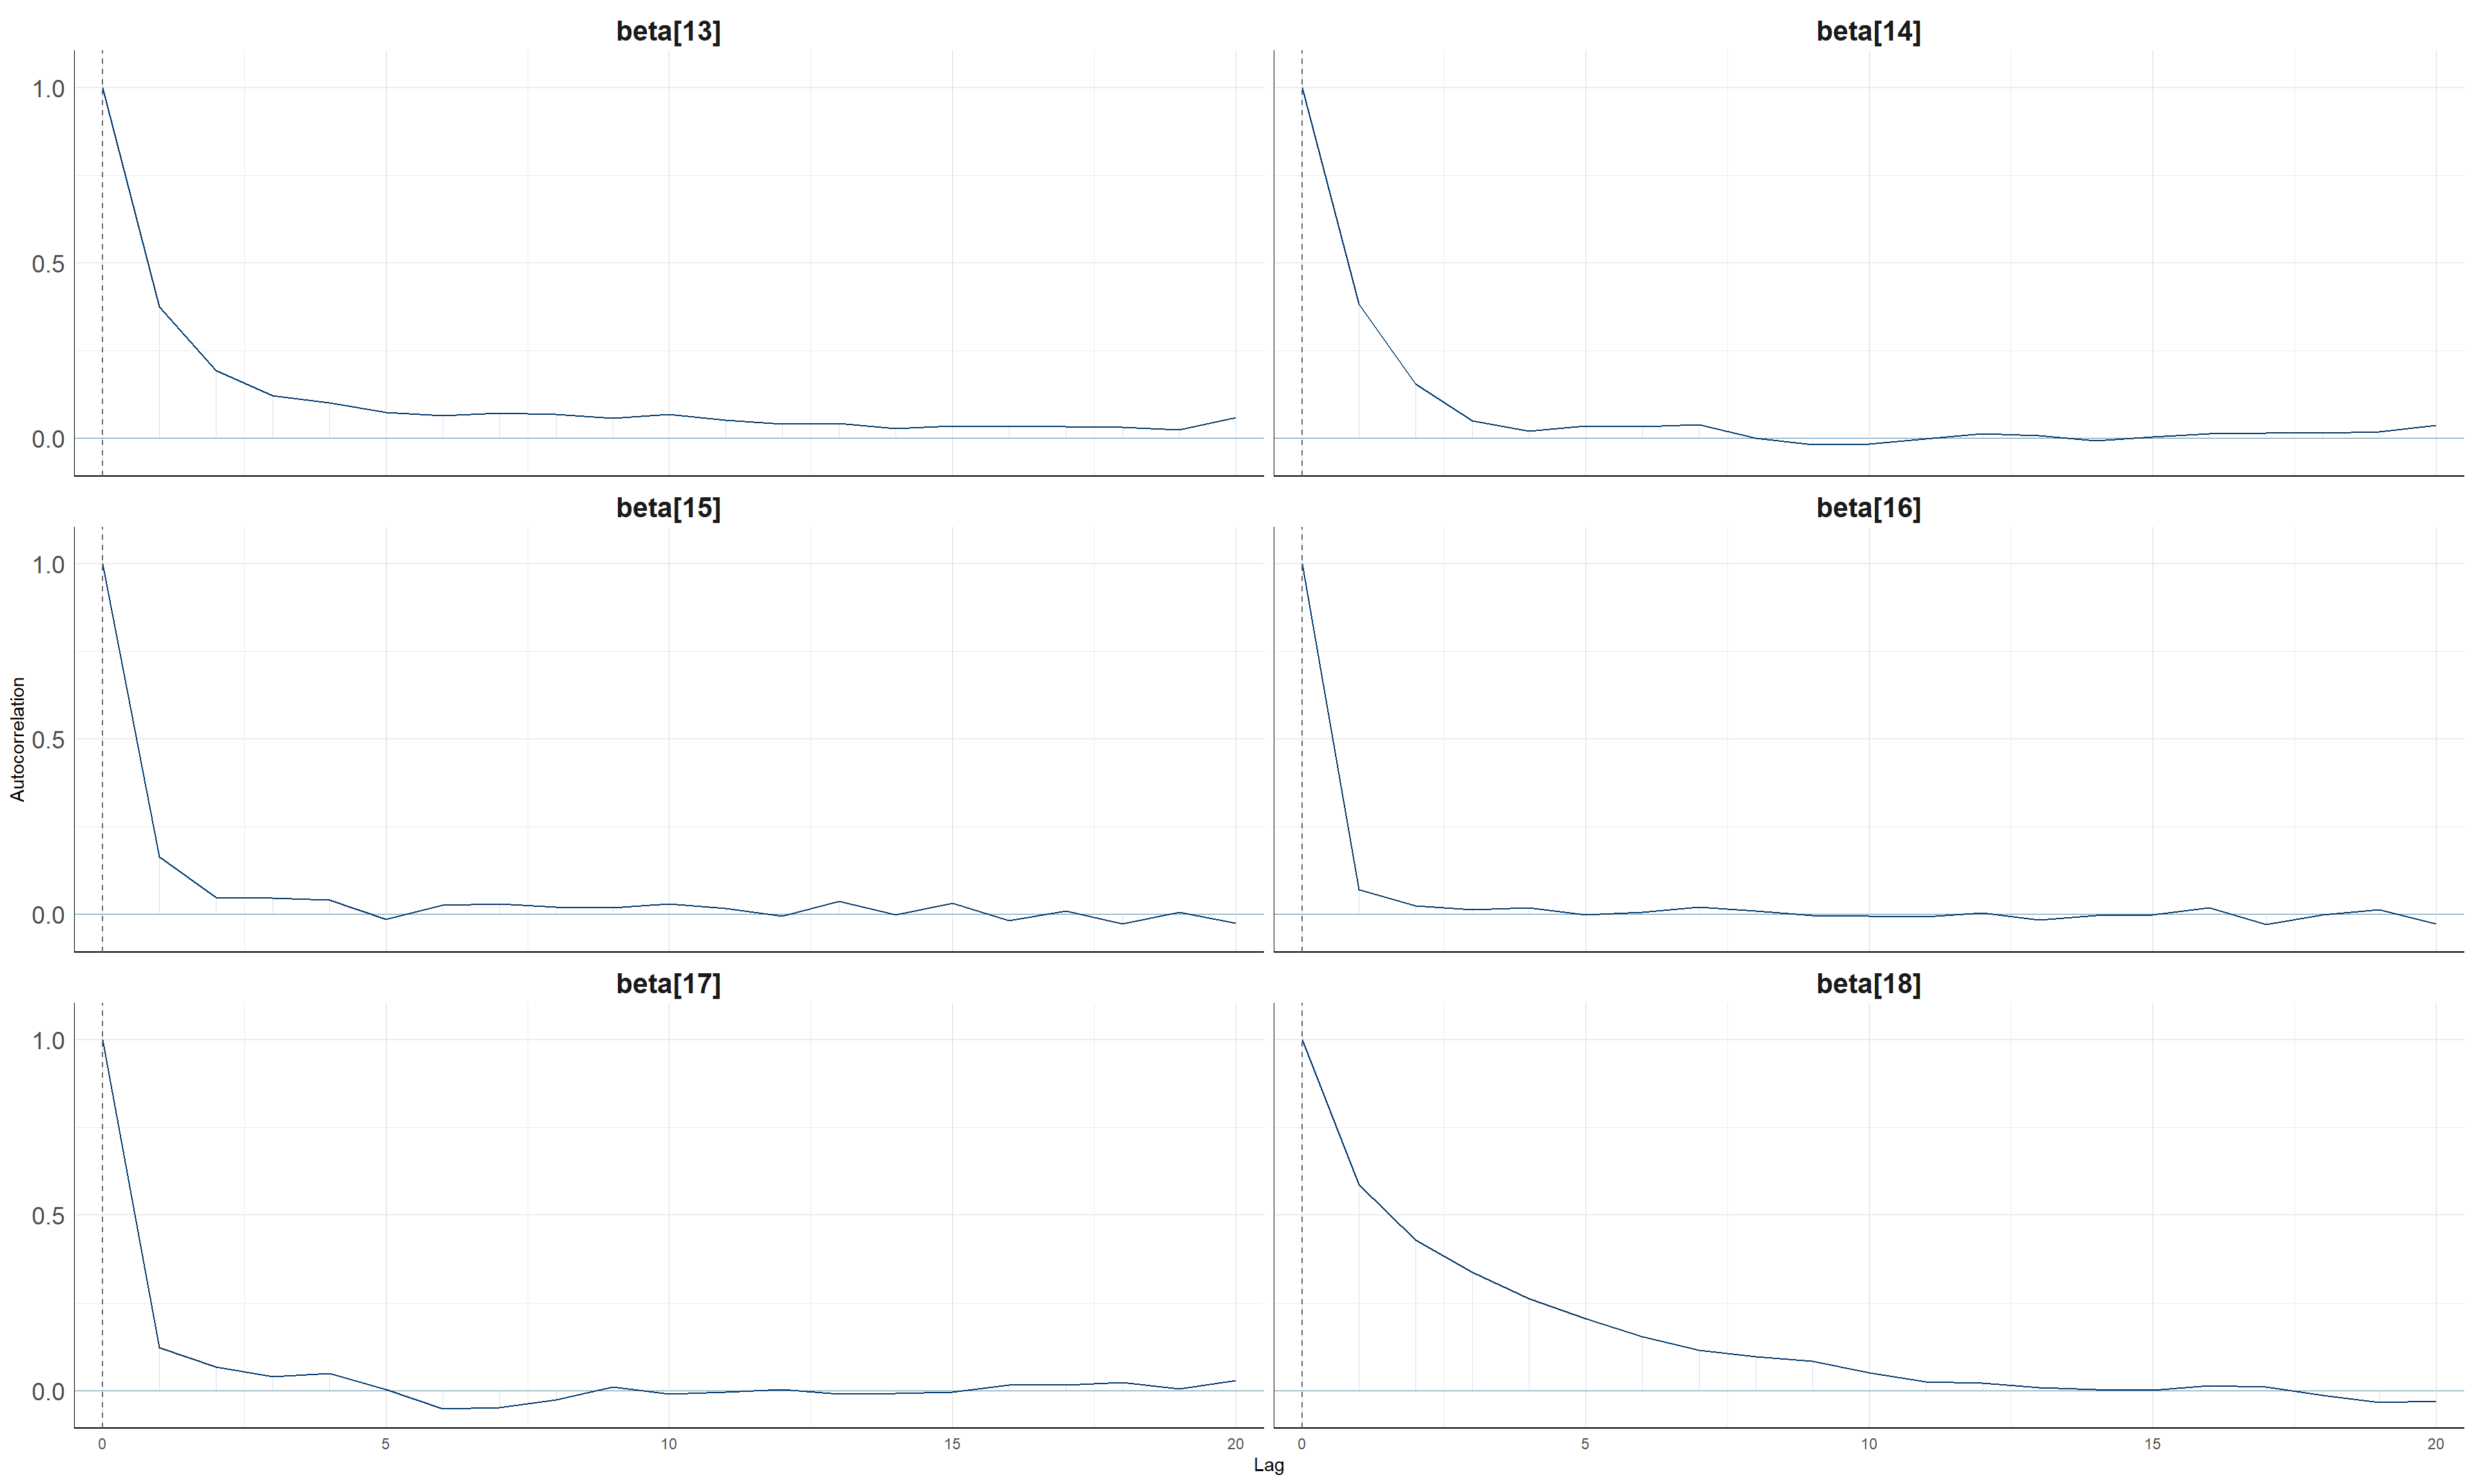
\includegraphics[width=\linewidth]{img/horseshoe_model/acf_beta_chain1_3.png}
    \caption{Group 3.}
  \end{subfigure}\hfill
  \begin{subfigure}[t]{0.48\linewidth}
    \centering
    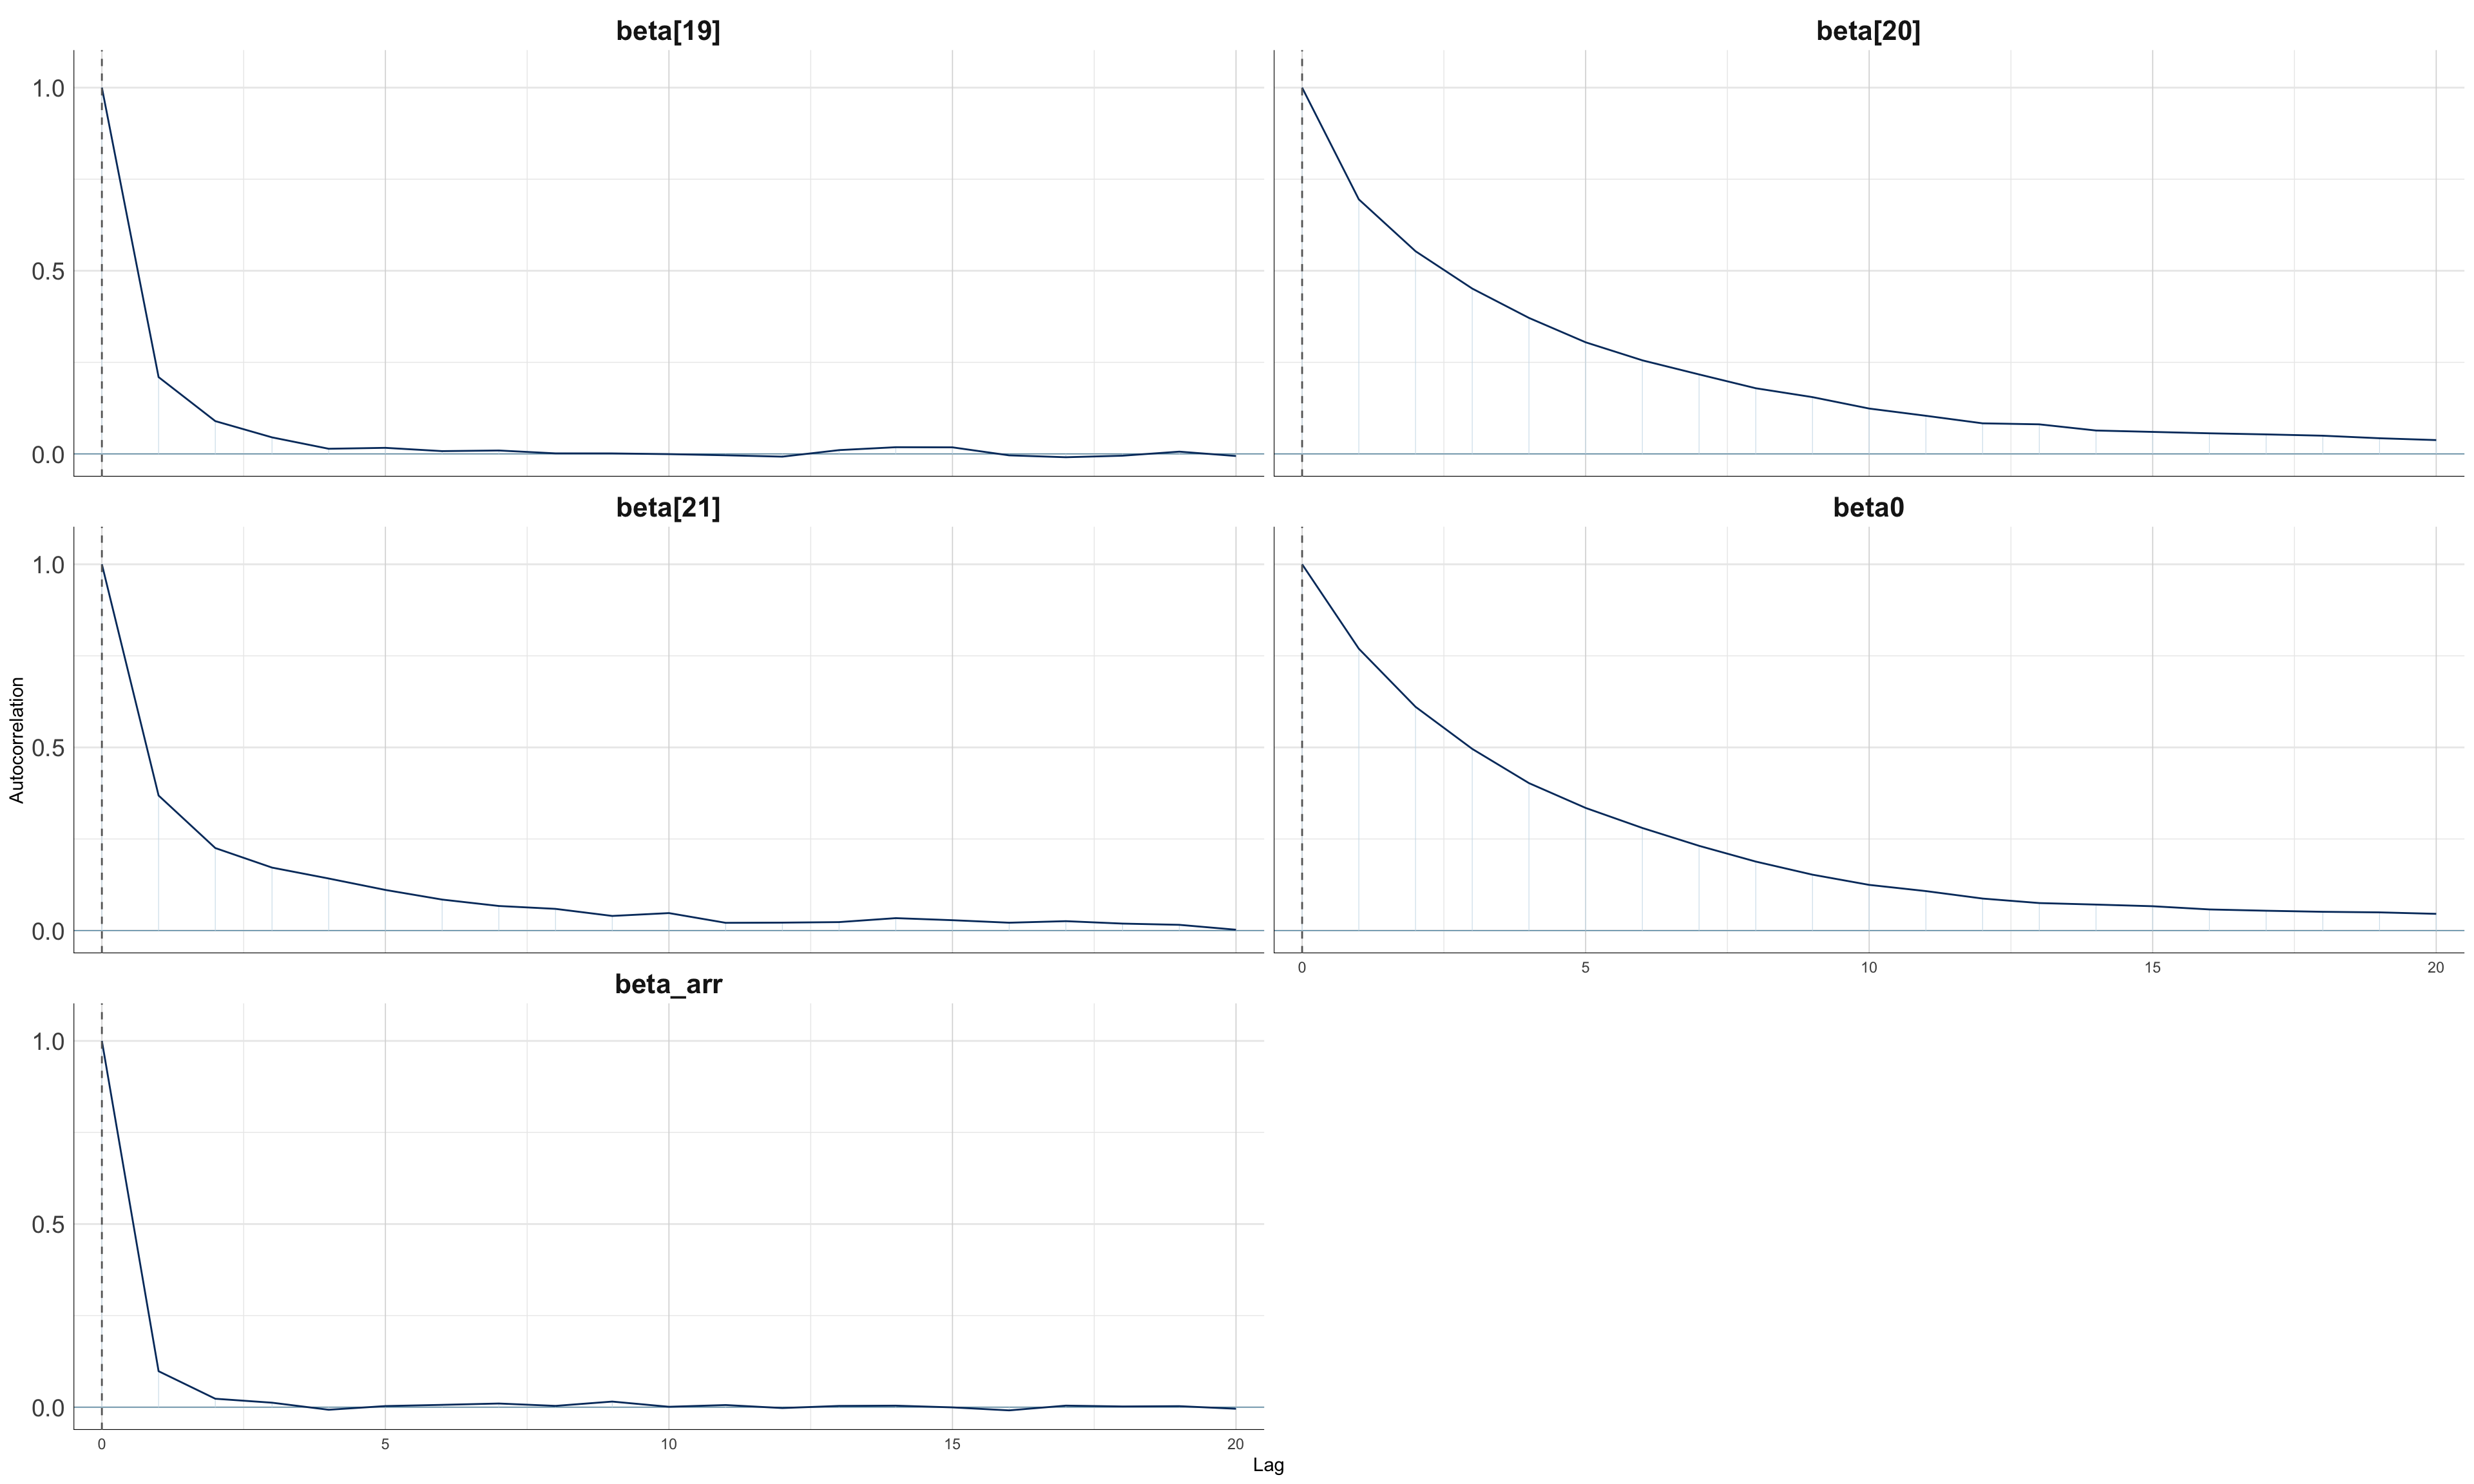
\includegraphics[width=\linewidth]{img/horseshoe_model/acf_beta_chain1_4.png}
    \caption{Group 4.}
  \end{subfigure}\hfill
  \caption{Autocorrelation of the coefficients $\beta_j$, chain 1.}
  \label{fig:hs_acf_beta_1}
\end{figure}

\begin{figure}[htbp]
  \centering
  \begin{subfigure}[t]{0.48\linewidth}
    \centering
    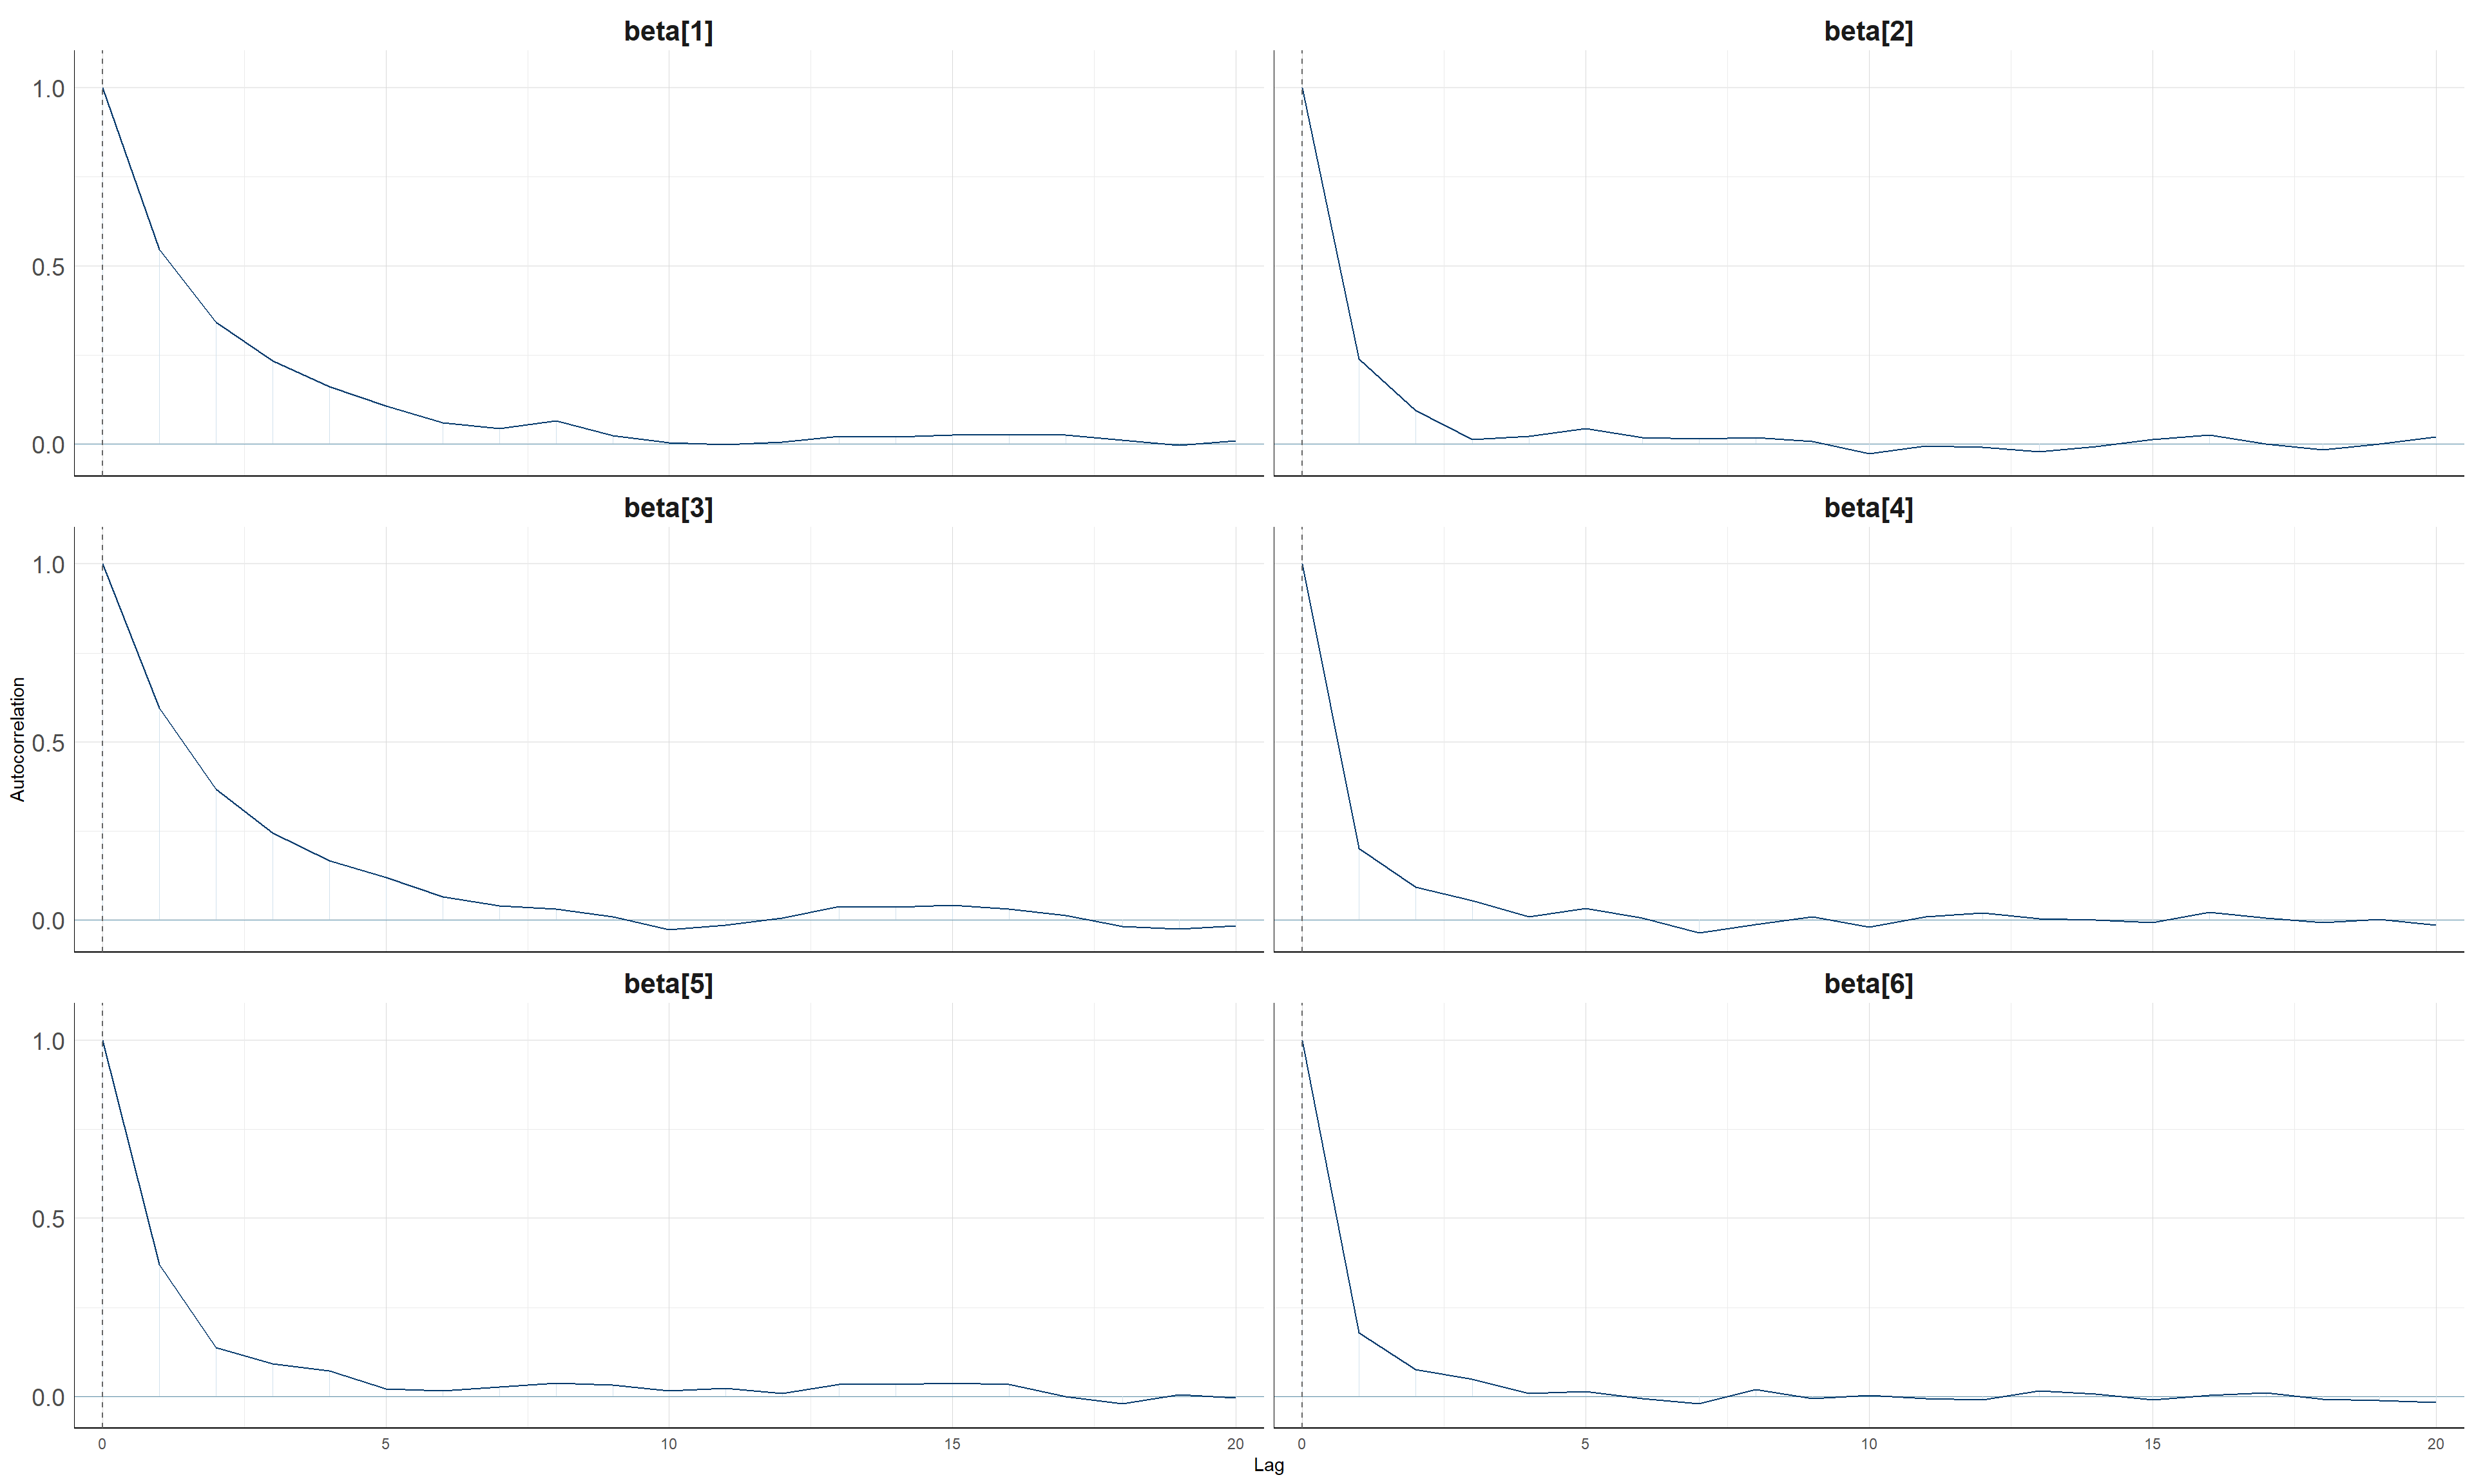
\includegraphics[width=\linewidth]{img/horseshoe_model/acf_beta_chain2_1.png}
    \caption{Group 1.}
  \end{subfigure}\hfill
  \begin{subfigure}[t]{0.48\linewidth}
    \centering
    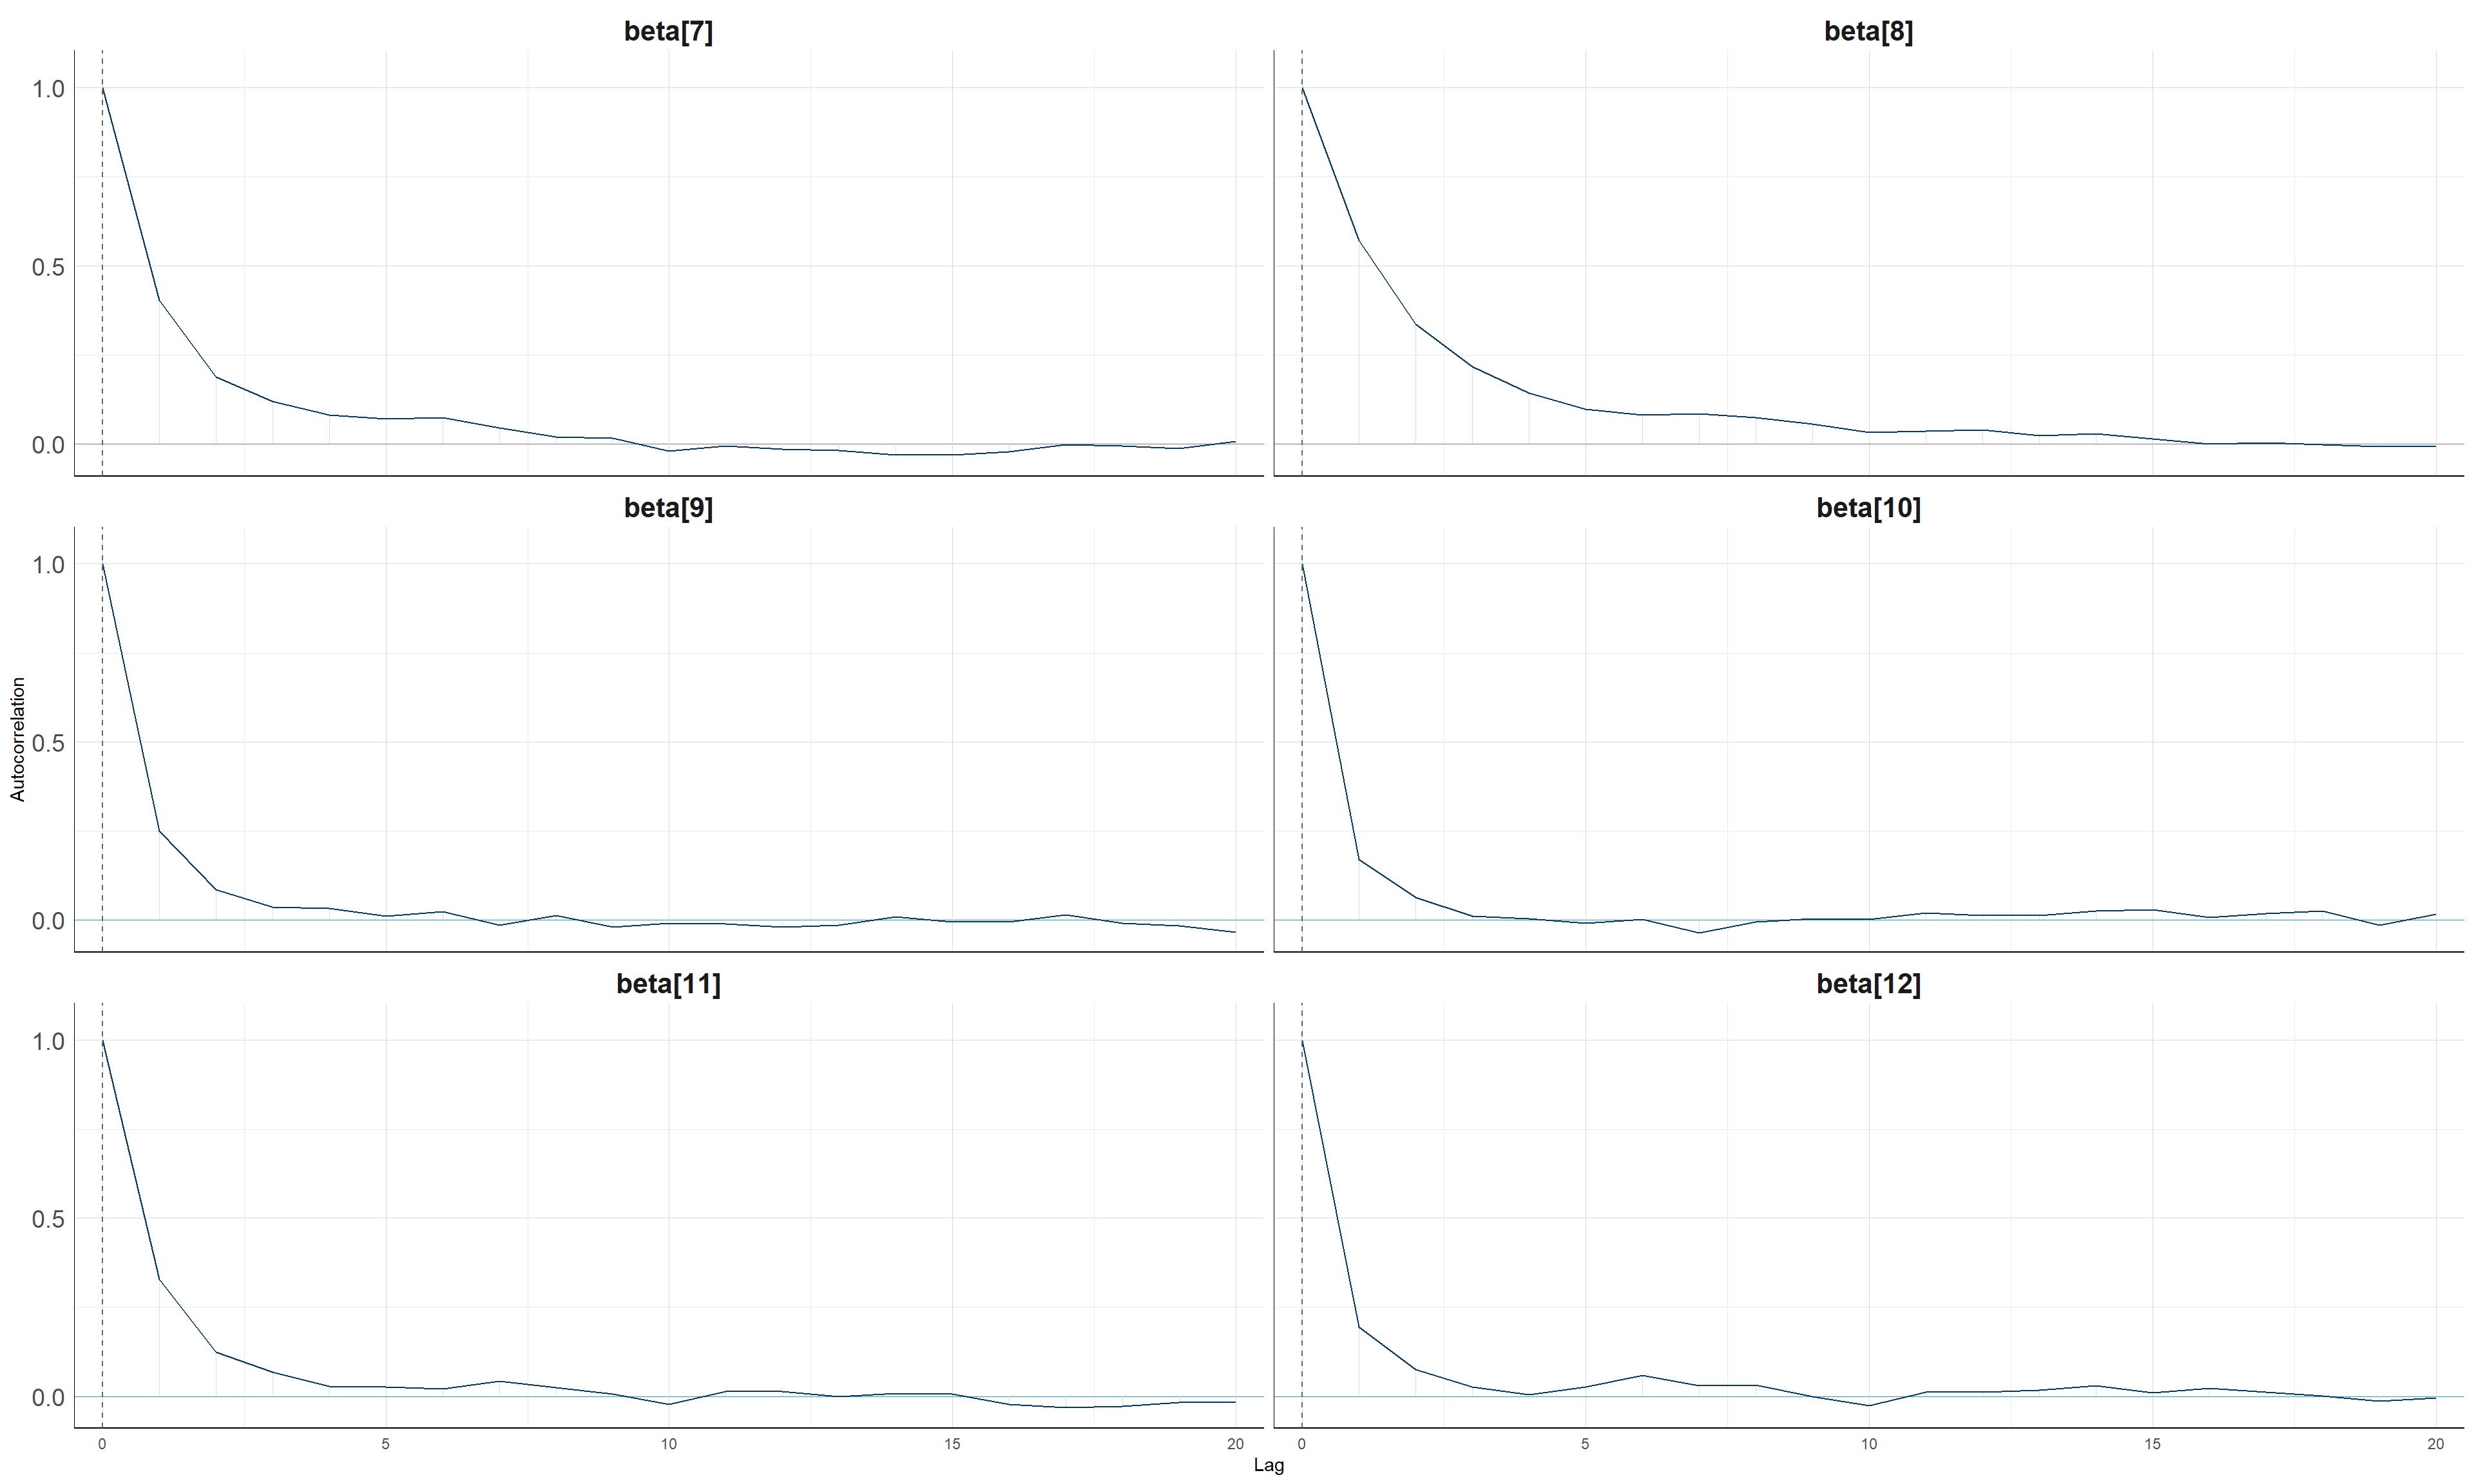
\includegraphics[width=\linewidth]{img/horseshoe_model/acf_beta_chain2_2.png}
    \caption{Group 2.}
  \end{subfigure}\hfill
  \begin{subfigure}[t]{0.48\linewidth}
    \centering
    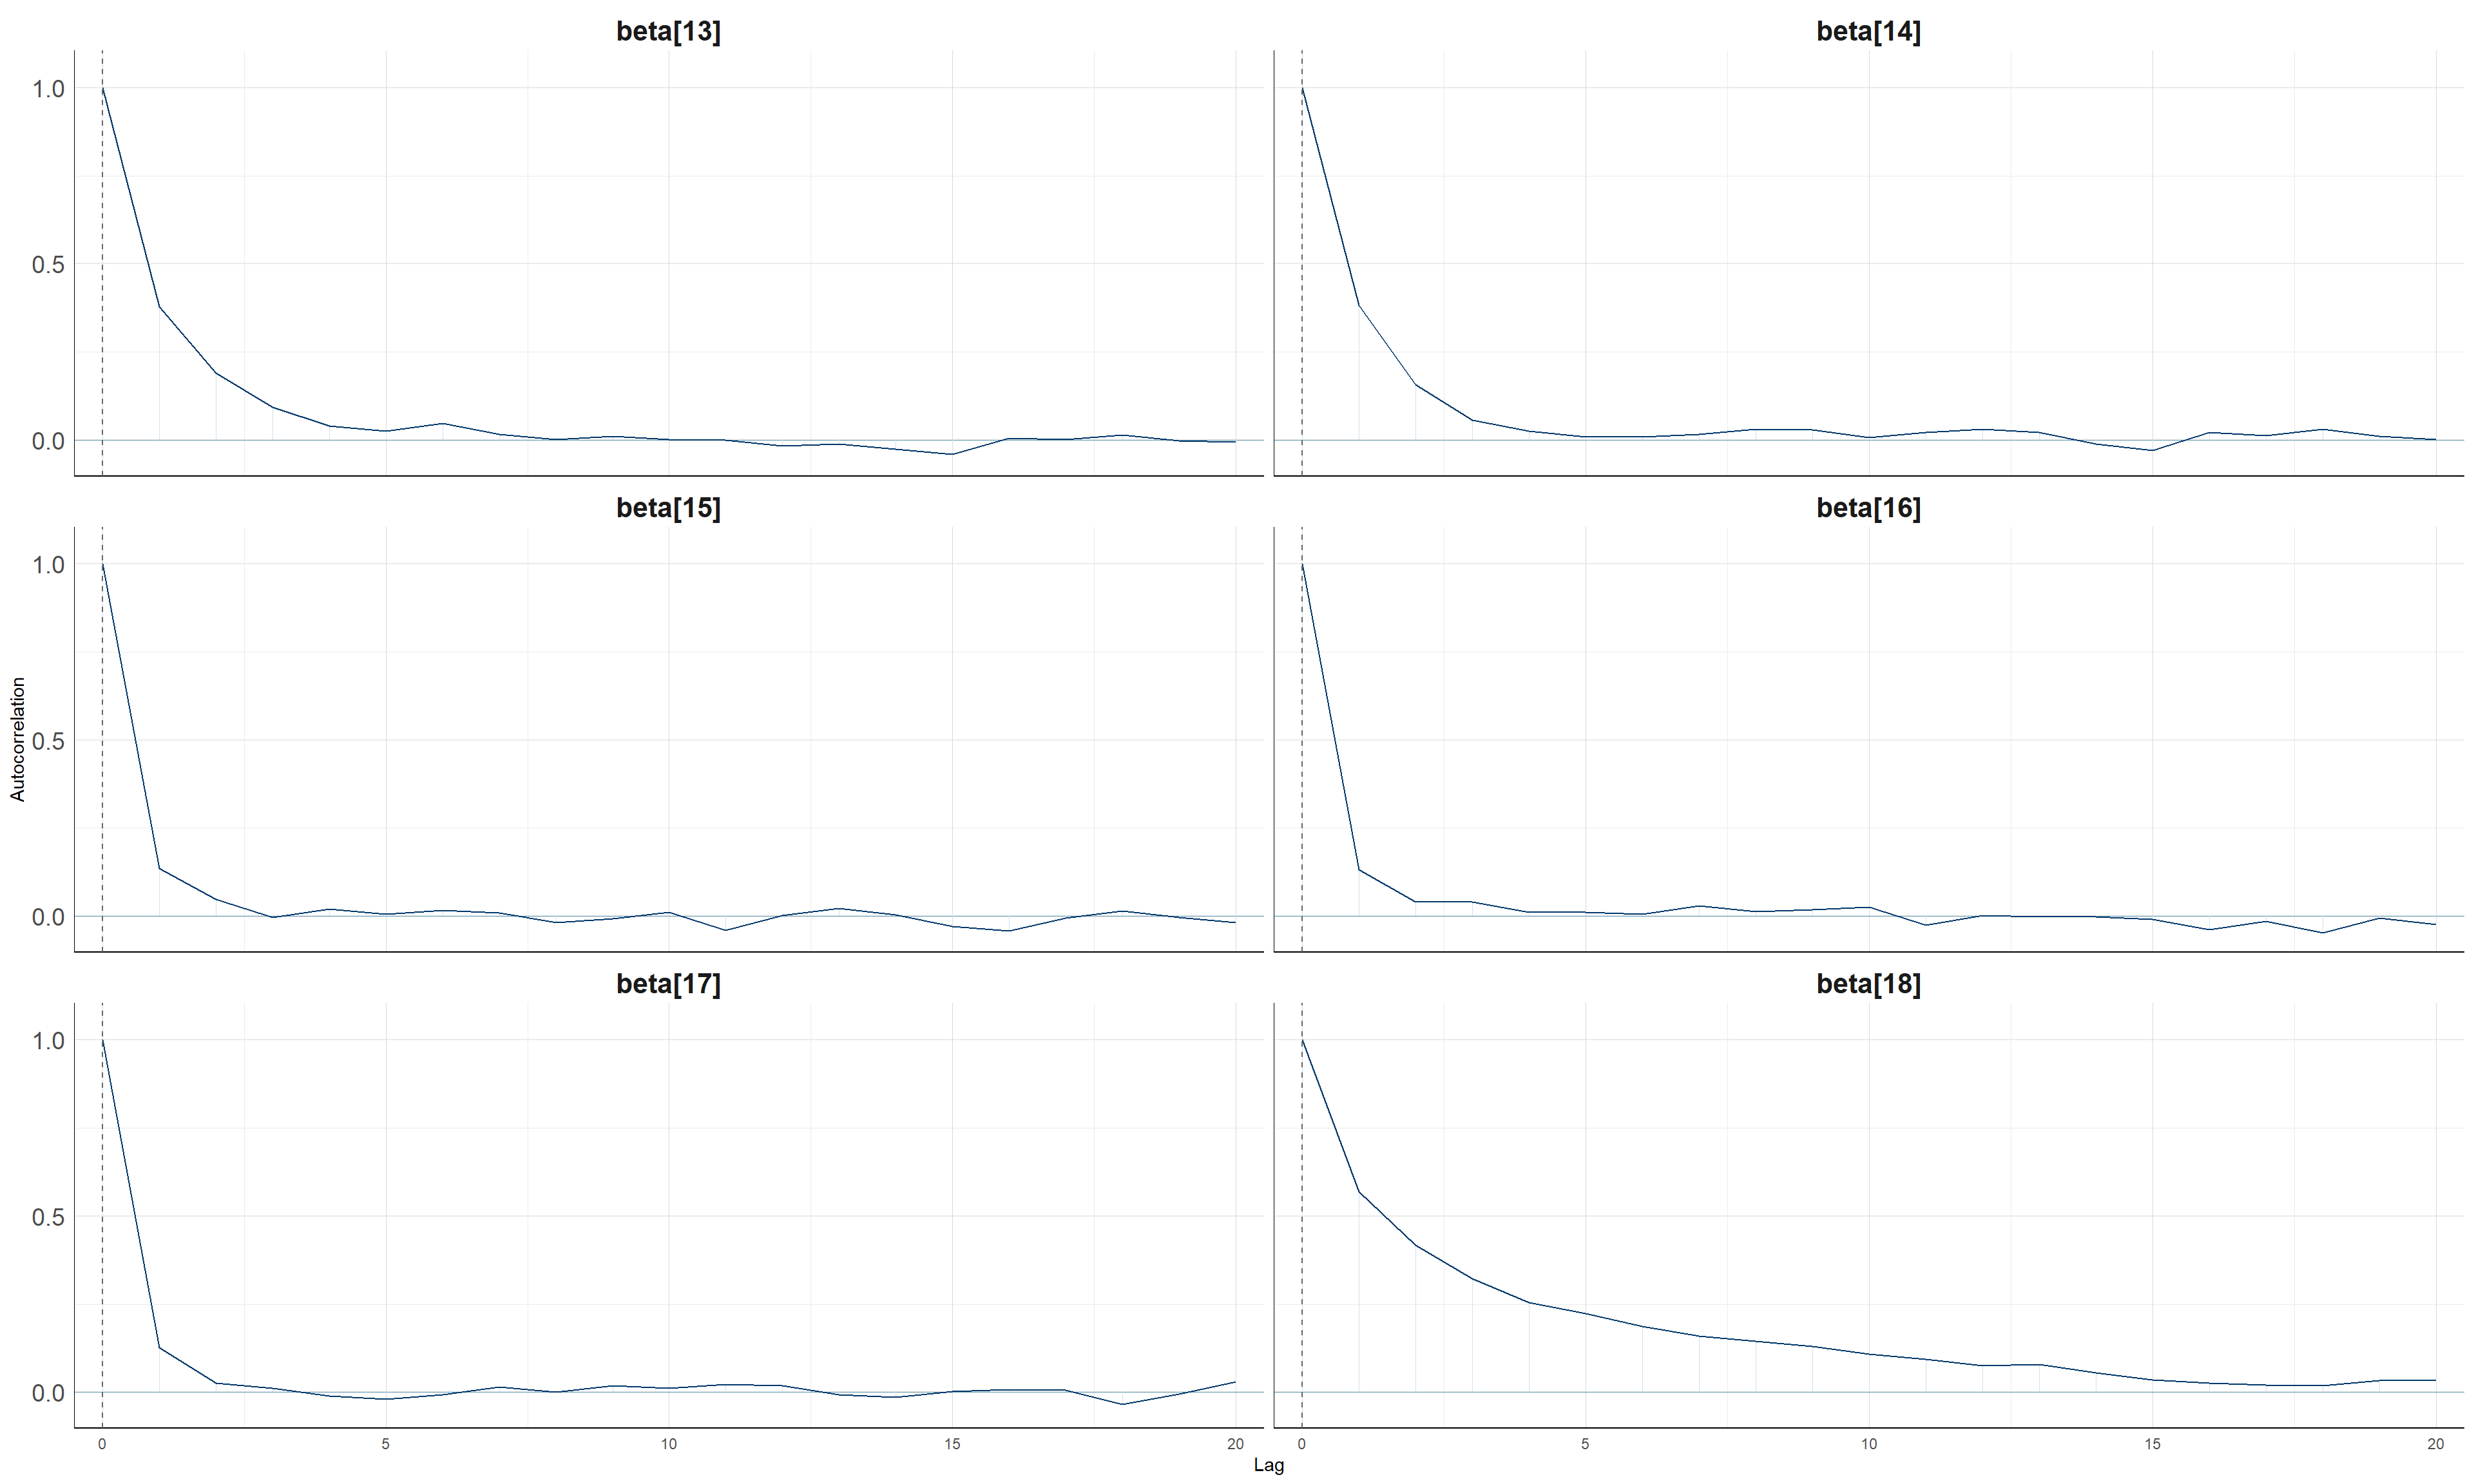
\includegraphics[width=\linewidth]{img/horseshoe_model/acf_beta_chain2_3.png}
    \caption{Group 3.}
  \end{subfigure}\hfill
  \begin{subfigure}[t]{0.48\linewidth}
    \centering
    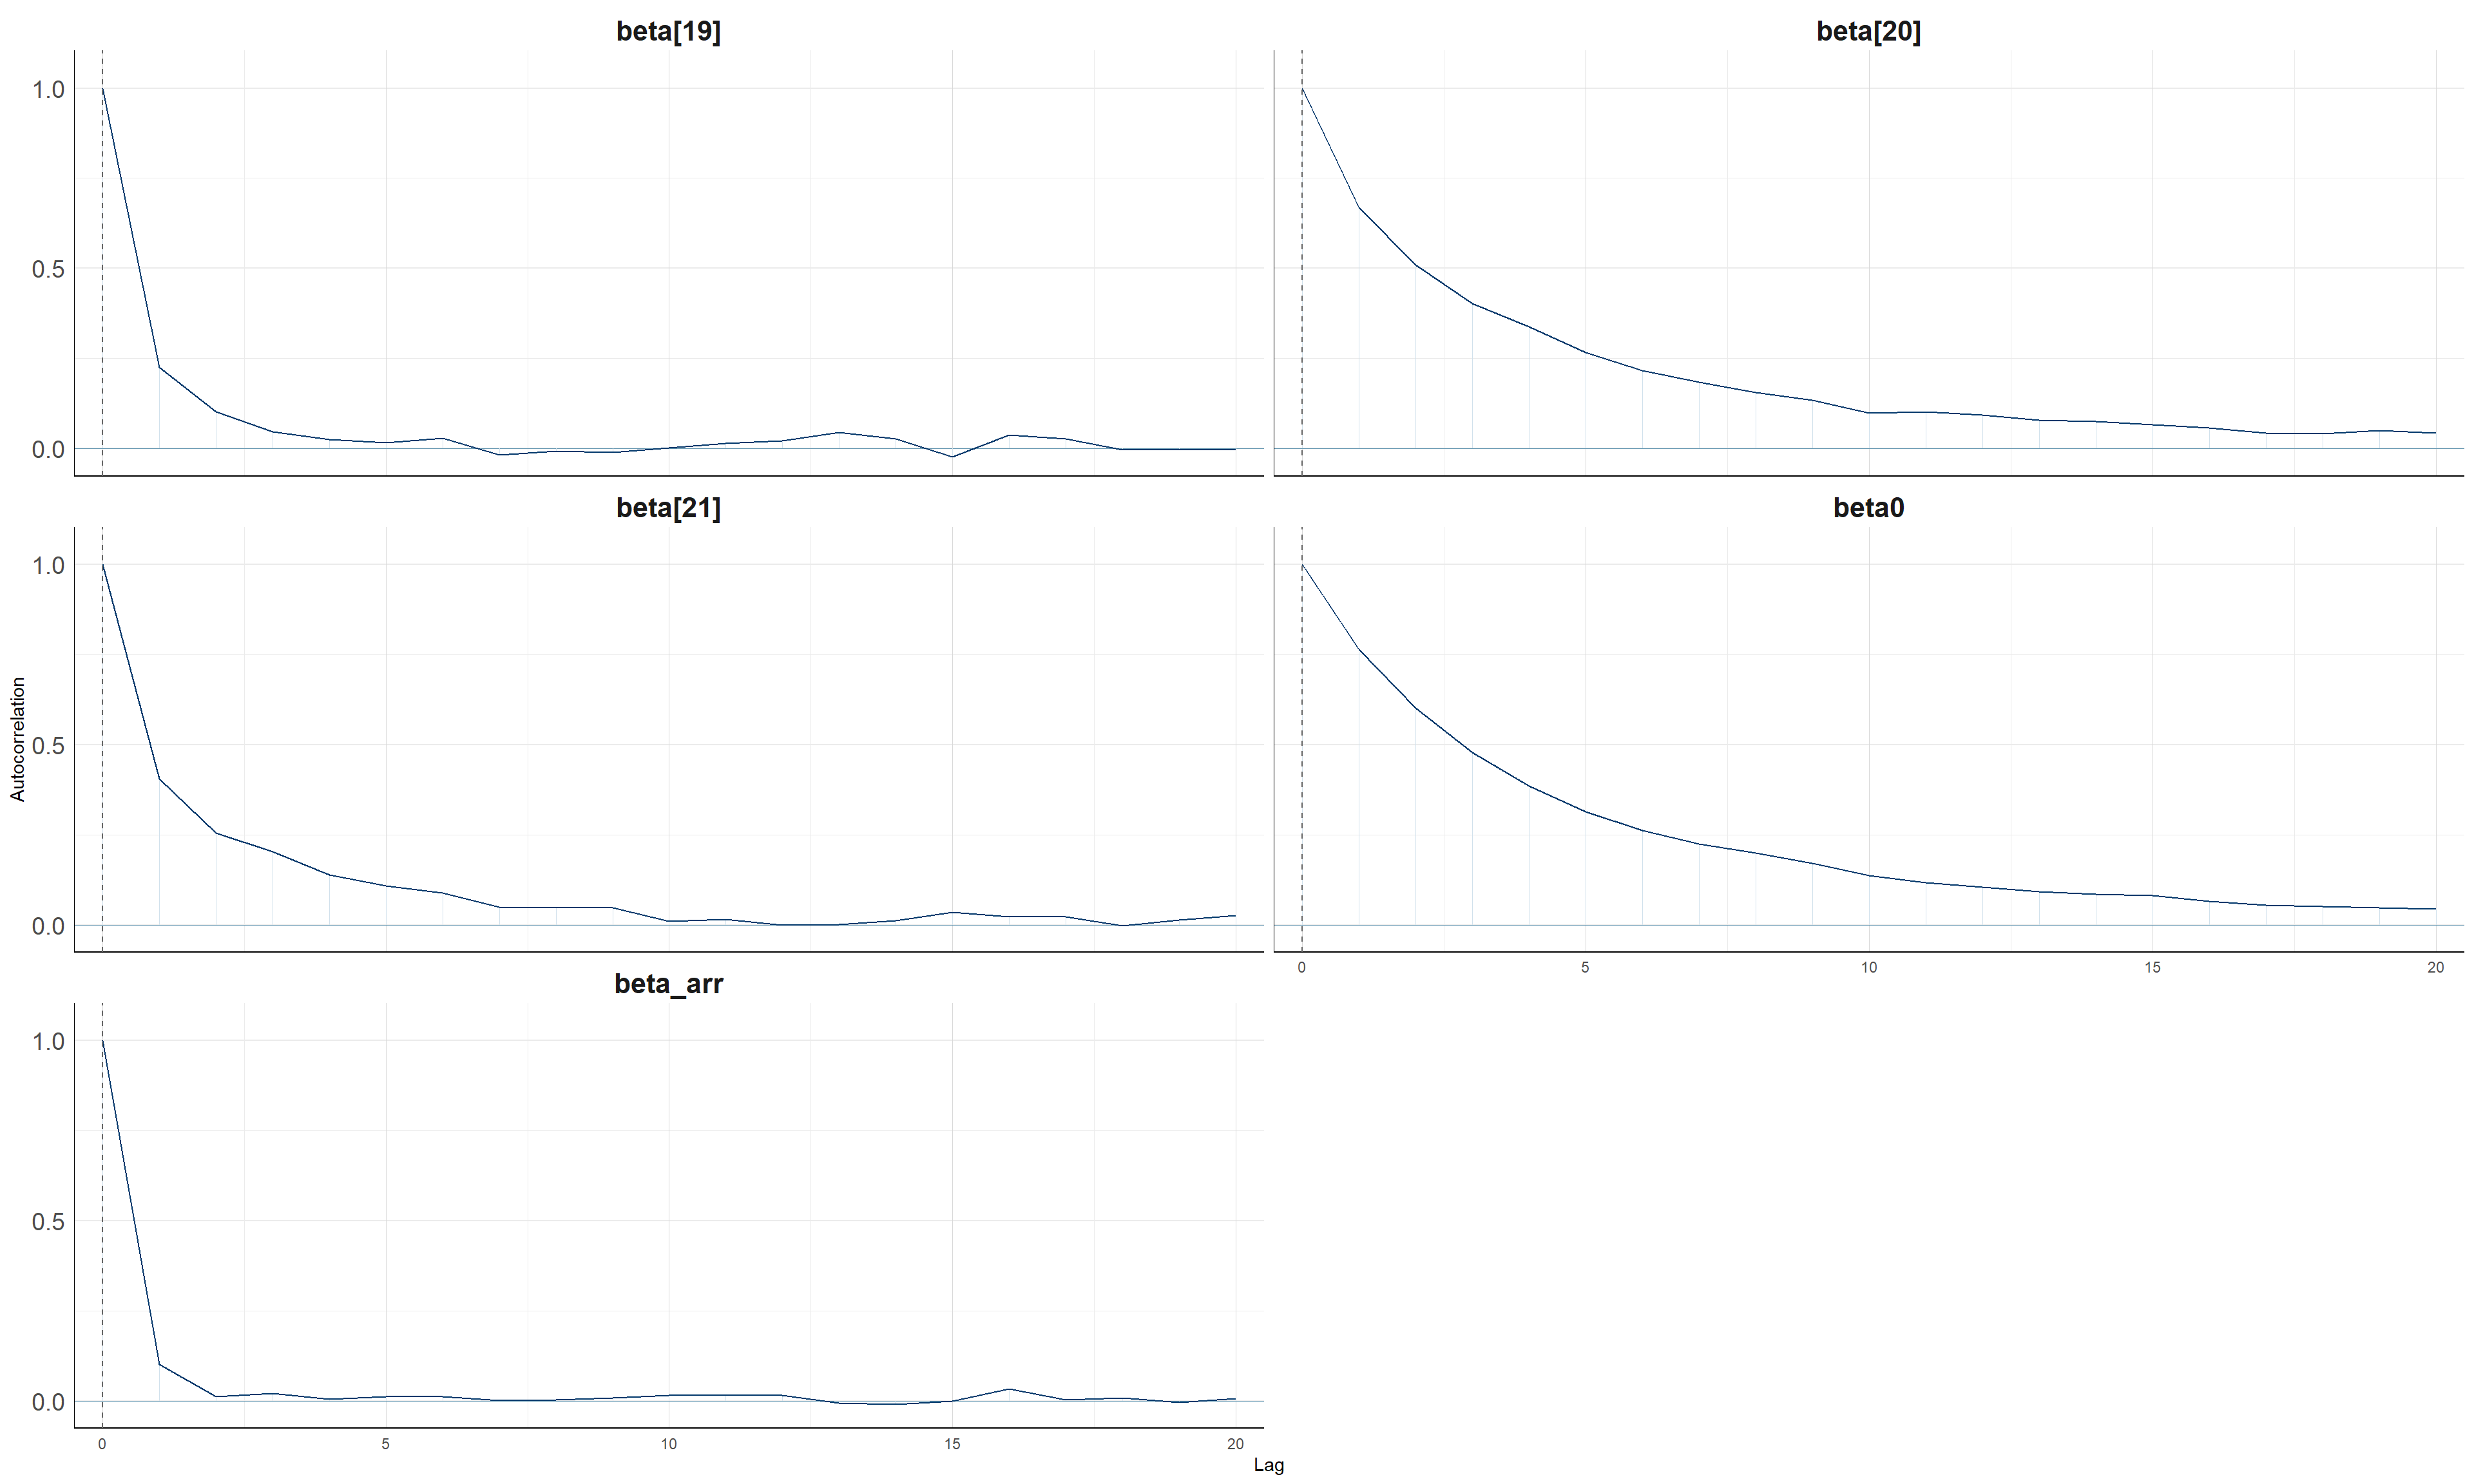
\includegraphics[width=\linewidth]{img/horseshoe_model/acf_beta_chain2_4.png}
    \caption{Group 4.}
  \end{subfigure}\hfill
  \caption{Autocorrelation of the coefficients $\beta_j$, chain 2.}
  \label{fig:hs_acf_beta_2}
\end{figure}

\begin{figure}[htbp]
  \centering
  \begin{subfigure}[t]{0.48\linewidth}
    \centering
    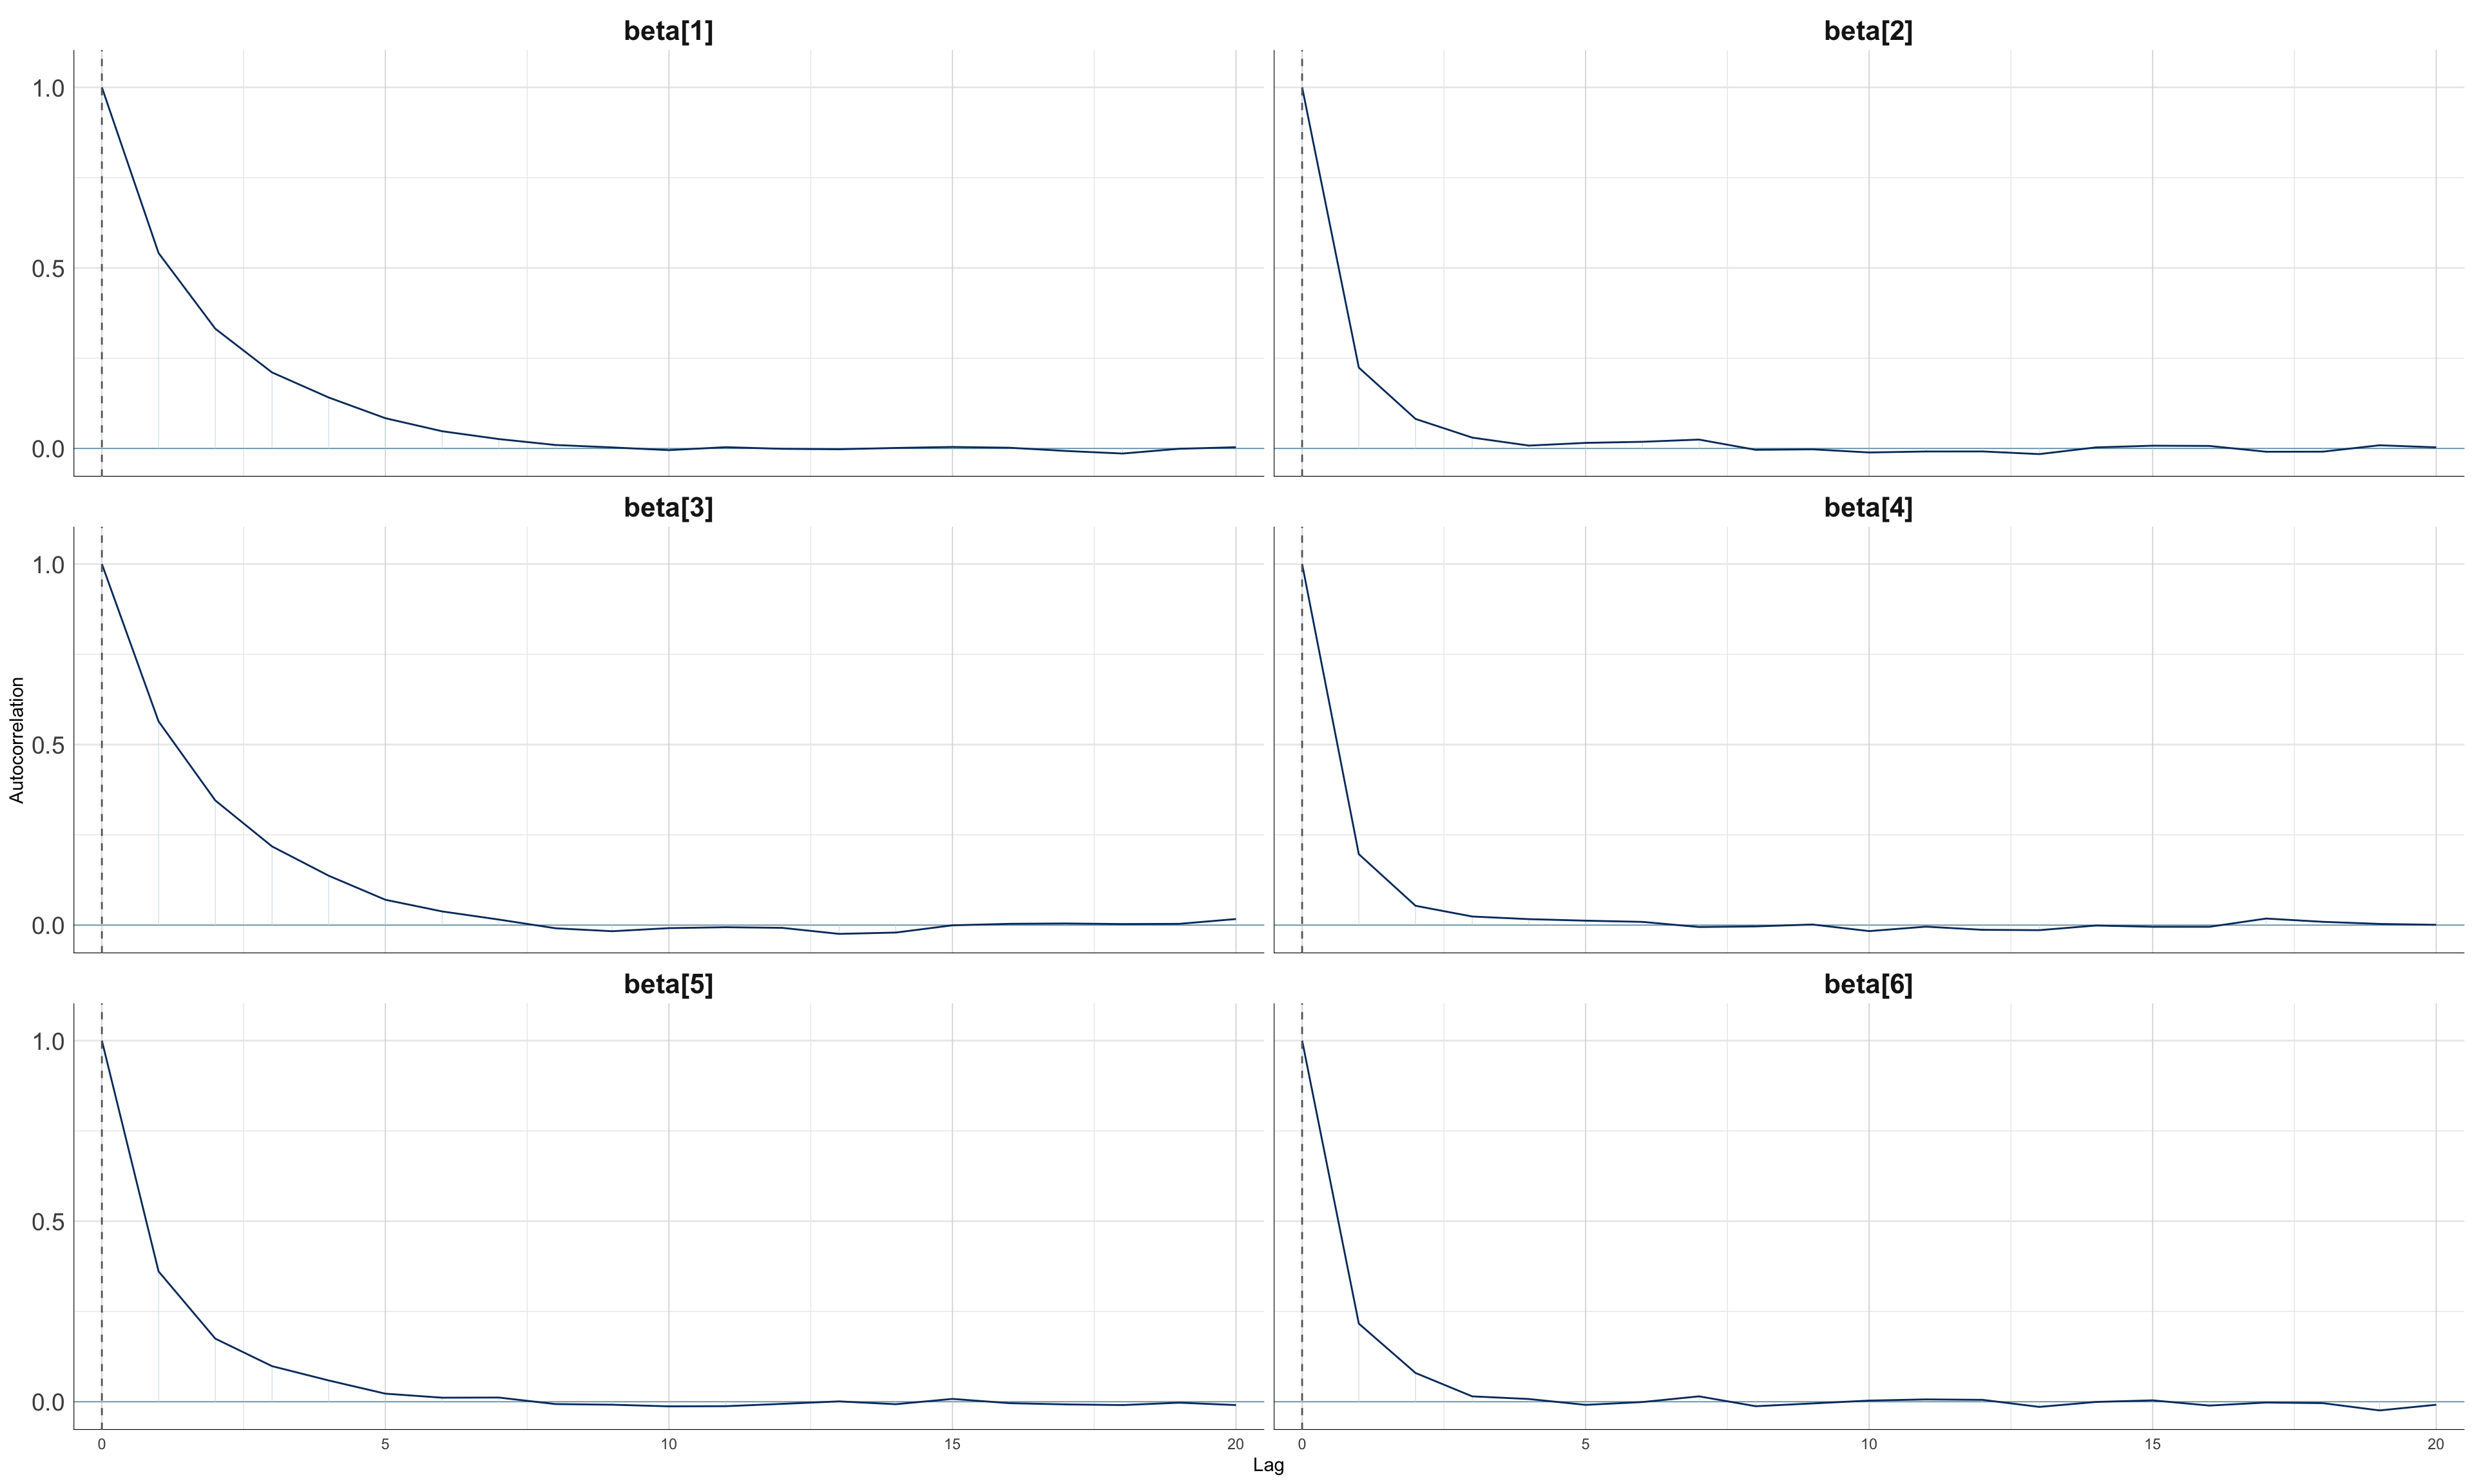
\includegraphics[width=\linewidth]{img/horseshoe_model/acf_beta_chain3_1.png}
    \caption{Group 1.}
  \end{subfigure}\hfill
  \begin{subfigure}[t]{0.48\linewidth}
    \centering
    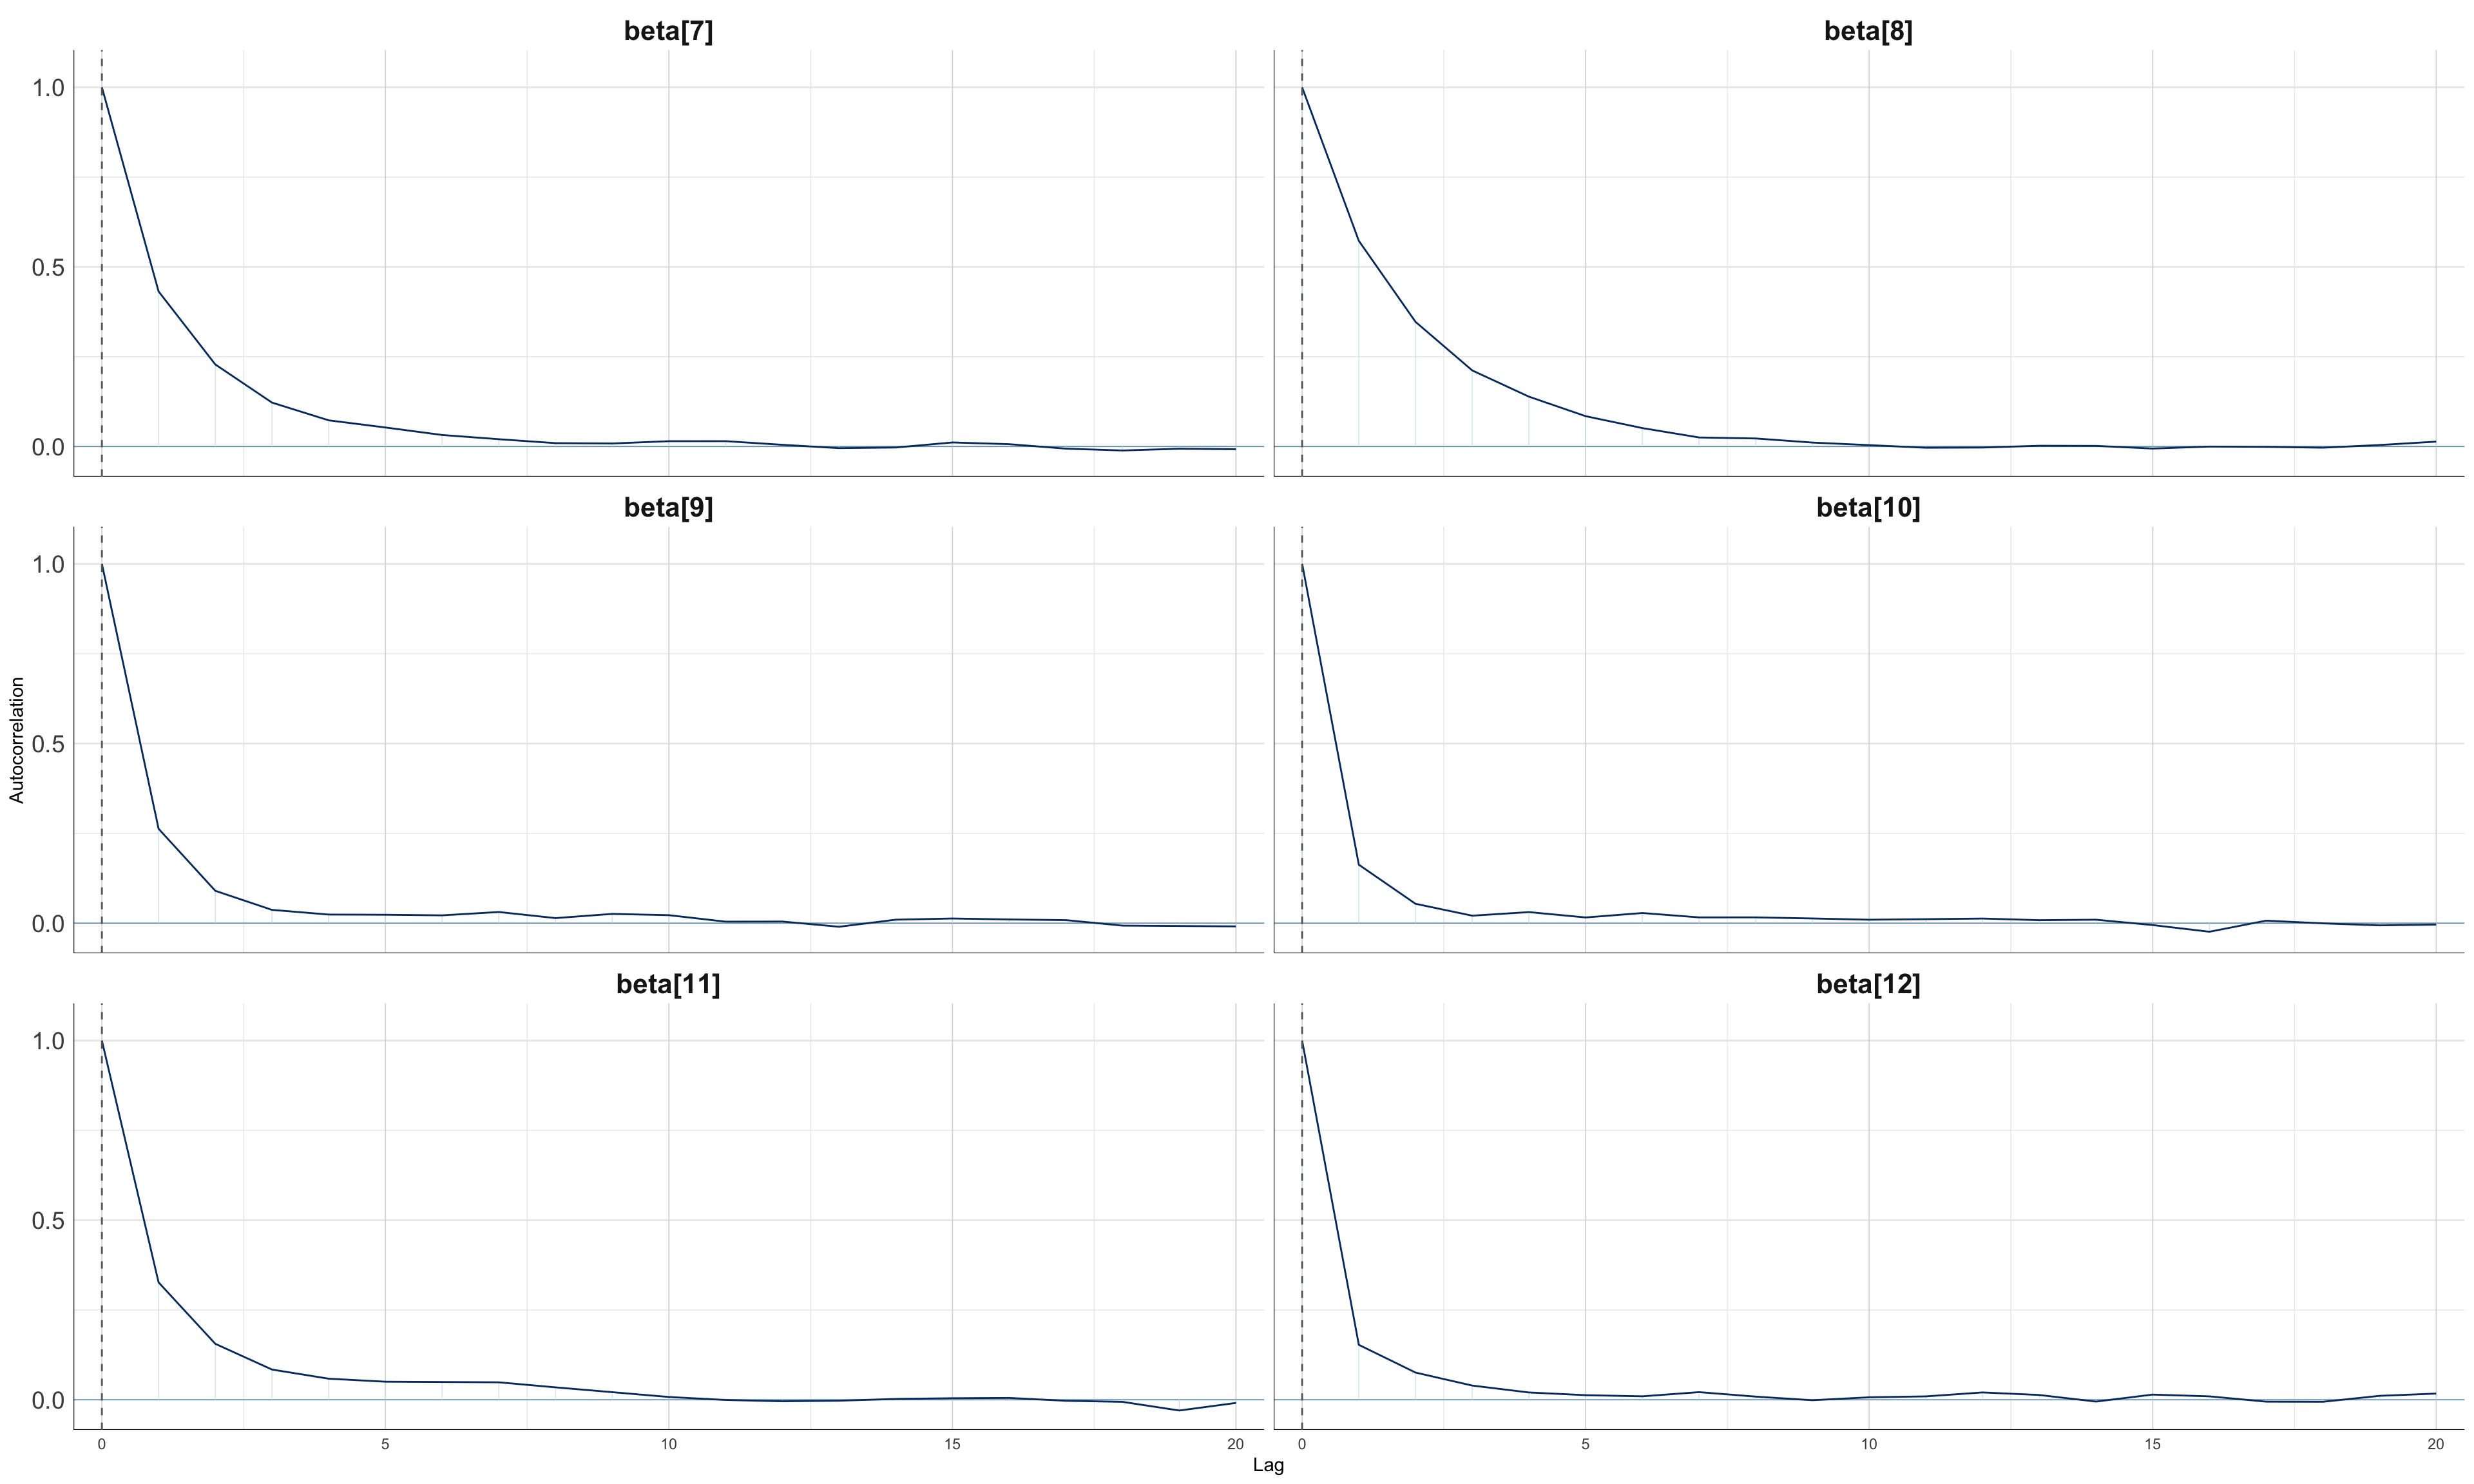
\includegraphics[width=\linewidth]{img/horseshoe_model/acf_beta_chain3_2.png}
    \caption{Group 2.}
  \end{subfigure}\hfill
  \begin{subfigure}[t]{0.48\linewidth}
    \centering
    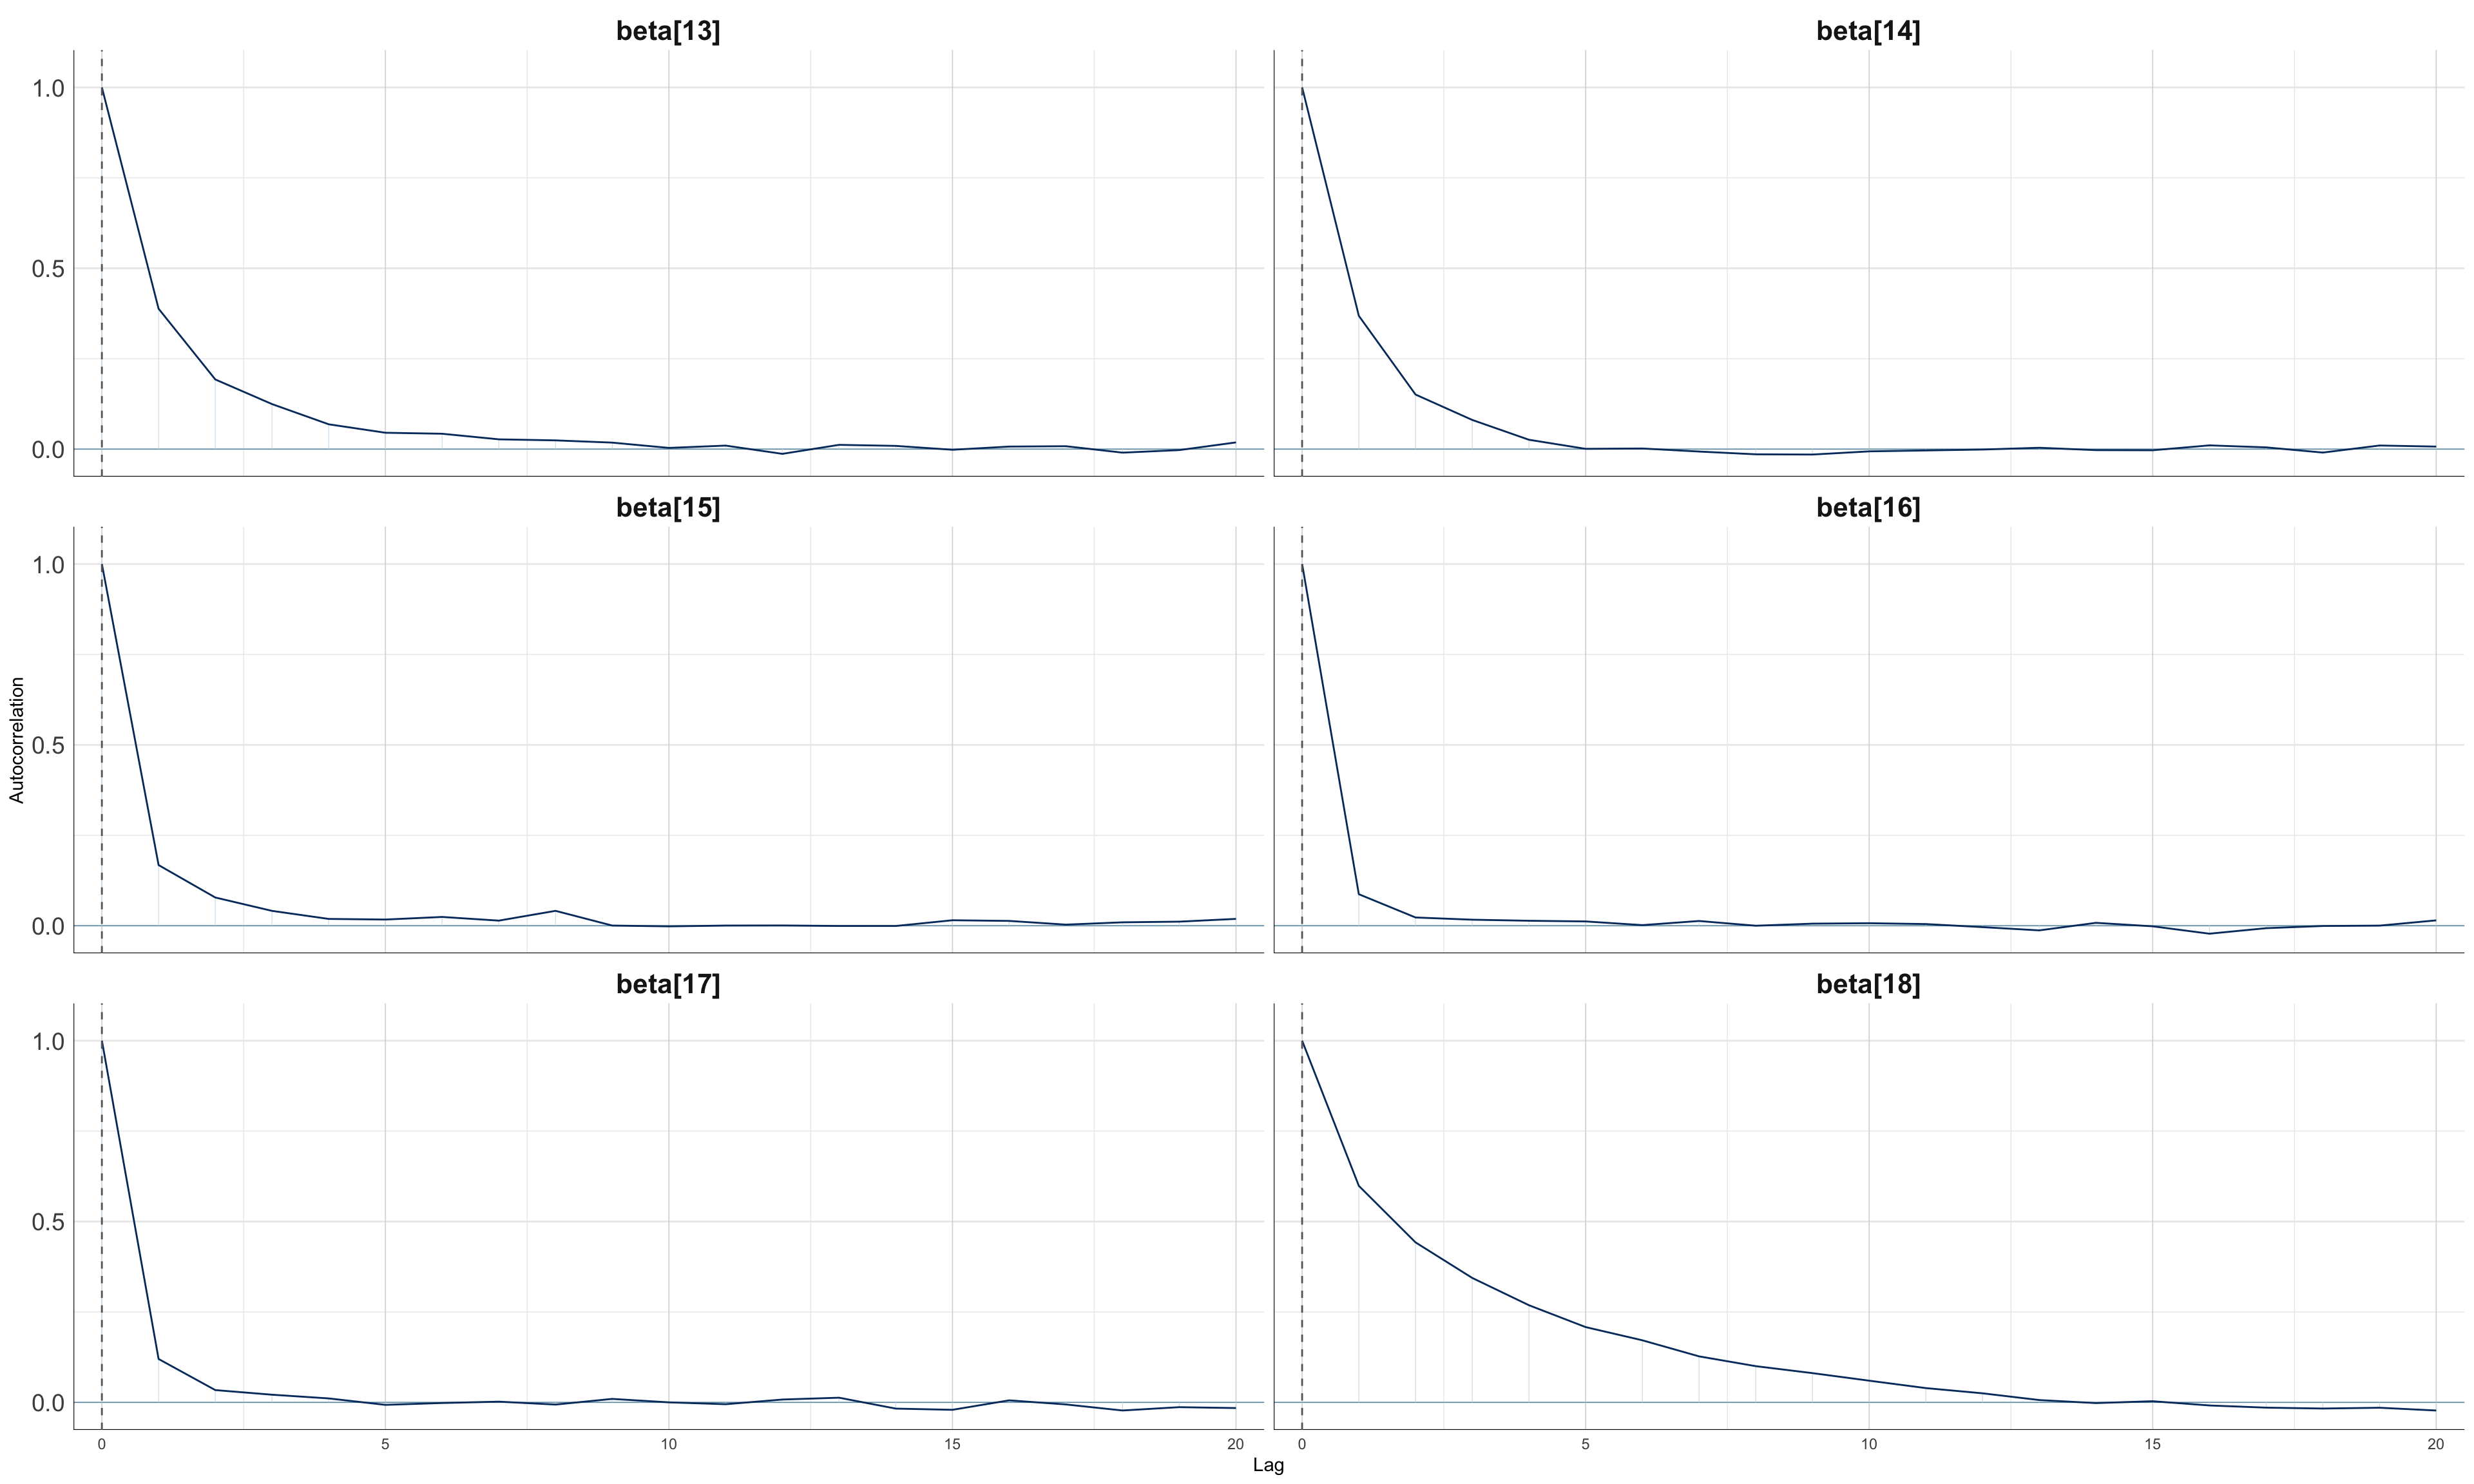
\includegraphics[width=\linewidth]{img/horseshoe_model/acf_beta_chain3_3.png}
    \caption{Group 3.}
  \end{subfigure}\hfill
  \begin{subfigure}[t]{0.48\linewidth}
    \centering
    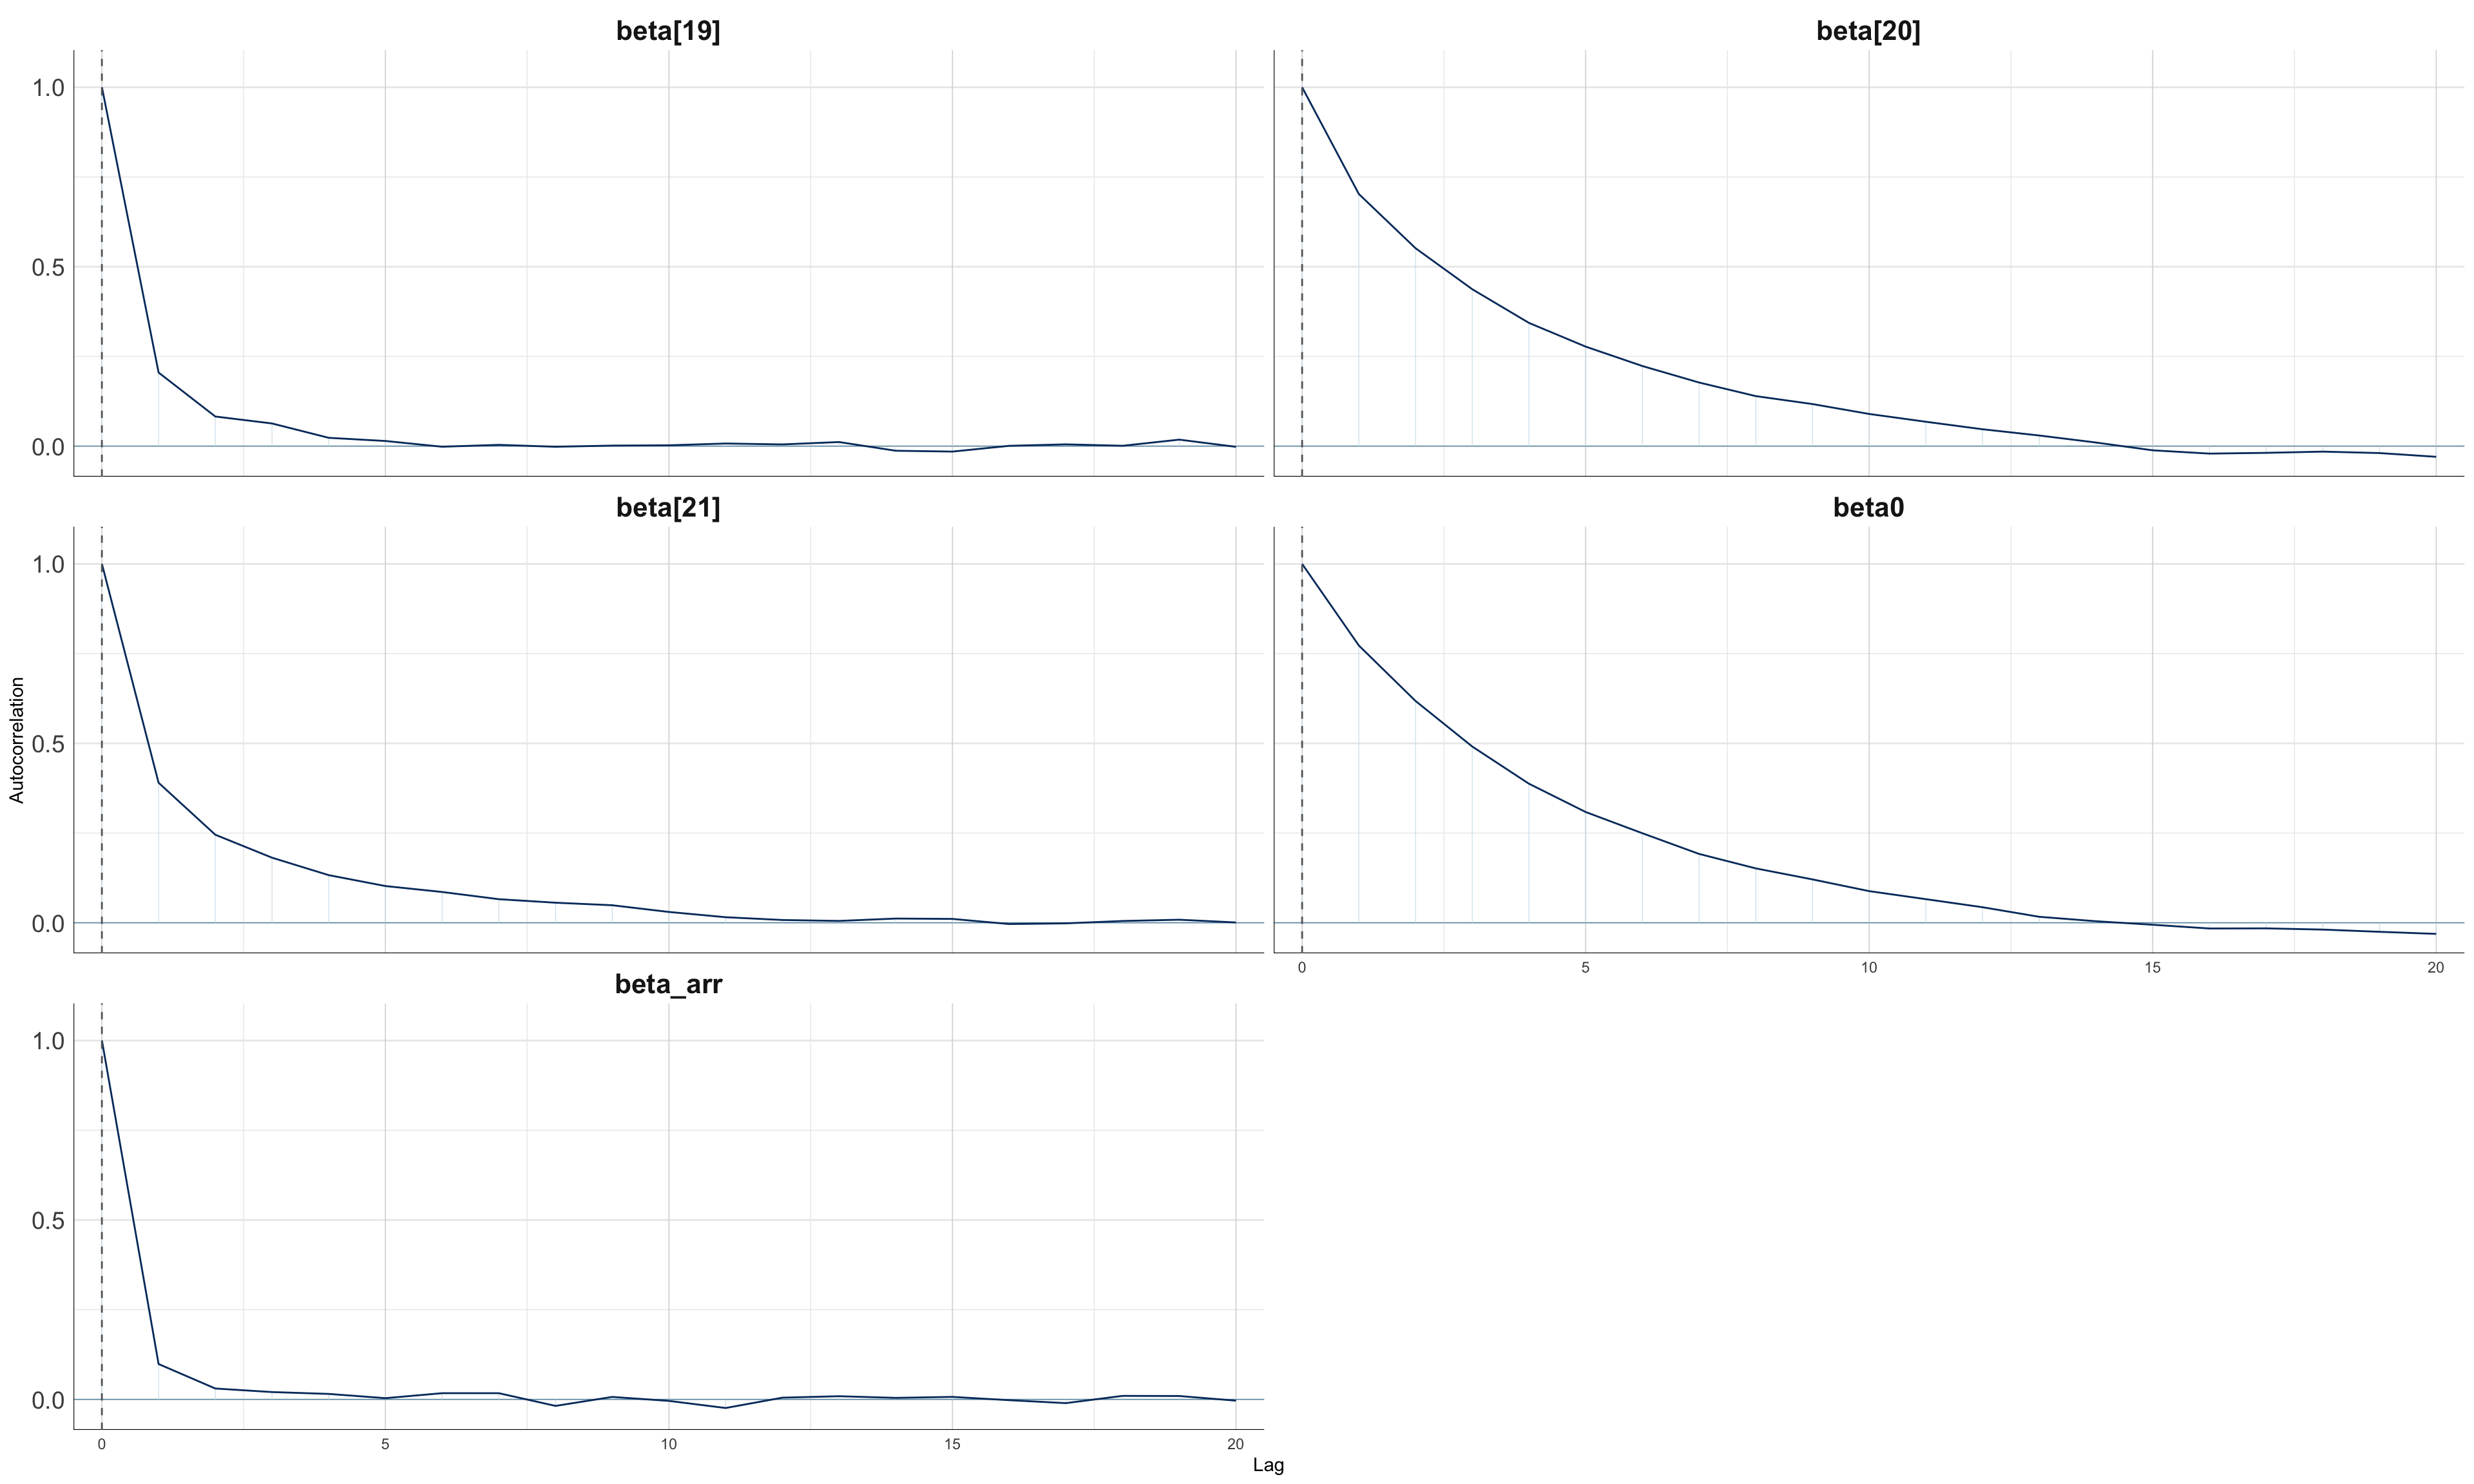
\includegraphics[width=\linewidth]{img/horseshoe_model/acf_beta_chain3_4.png}
    \caption{Group 4.}
  \end{subfigure}\hfill
  \caption{Autocorrelation of the coefficients $\beta_j$, chain 3.}
  \label{fig:hs_acf_beta_3}
\end{figure}

\begin{figure}[htbp]
  \centering
  \begin{subfigure}[t]{0.48\linewidth}
    \centering
    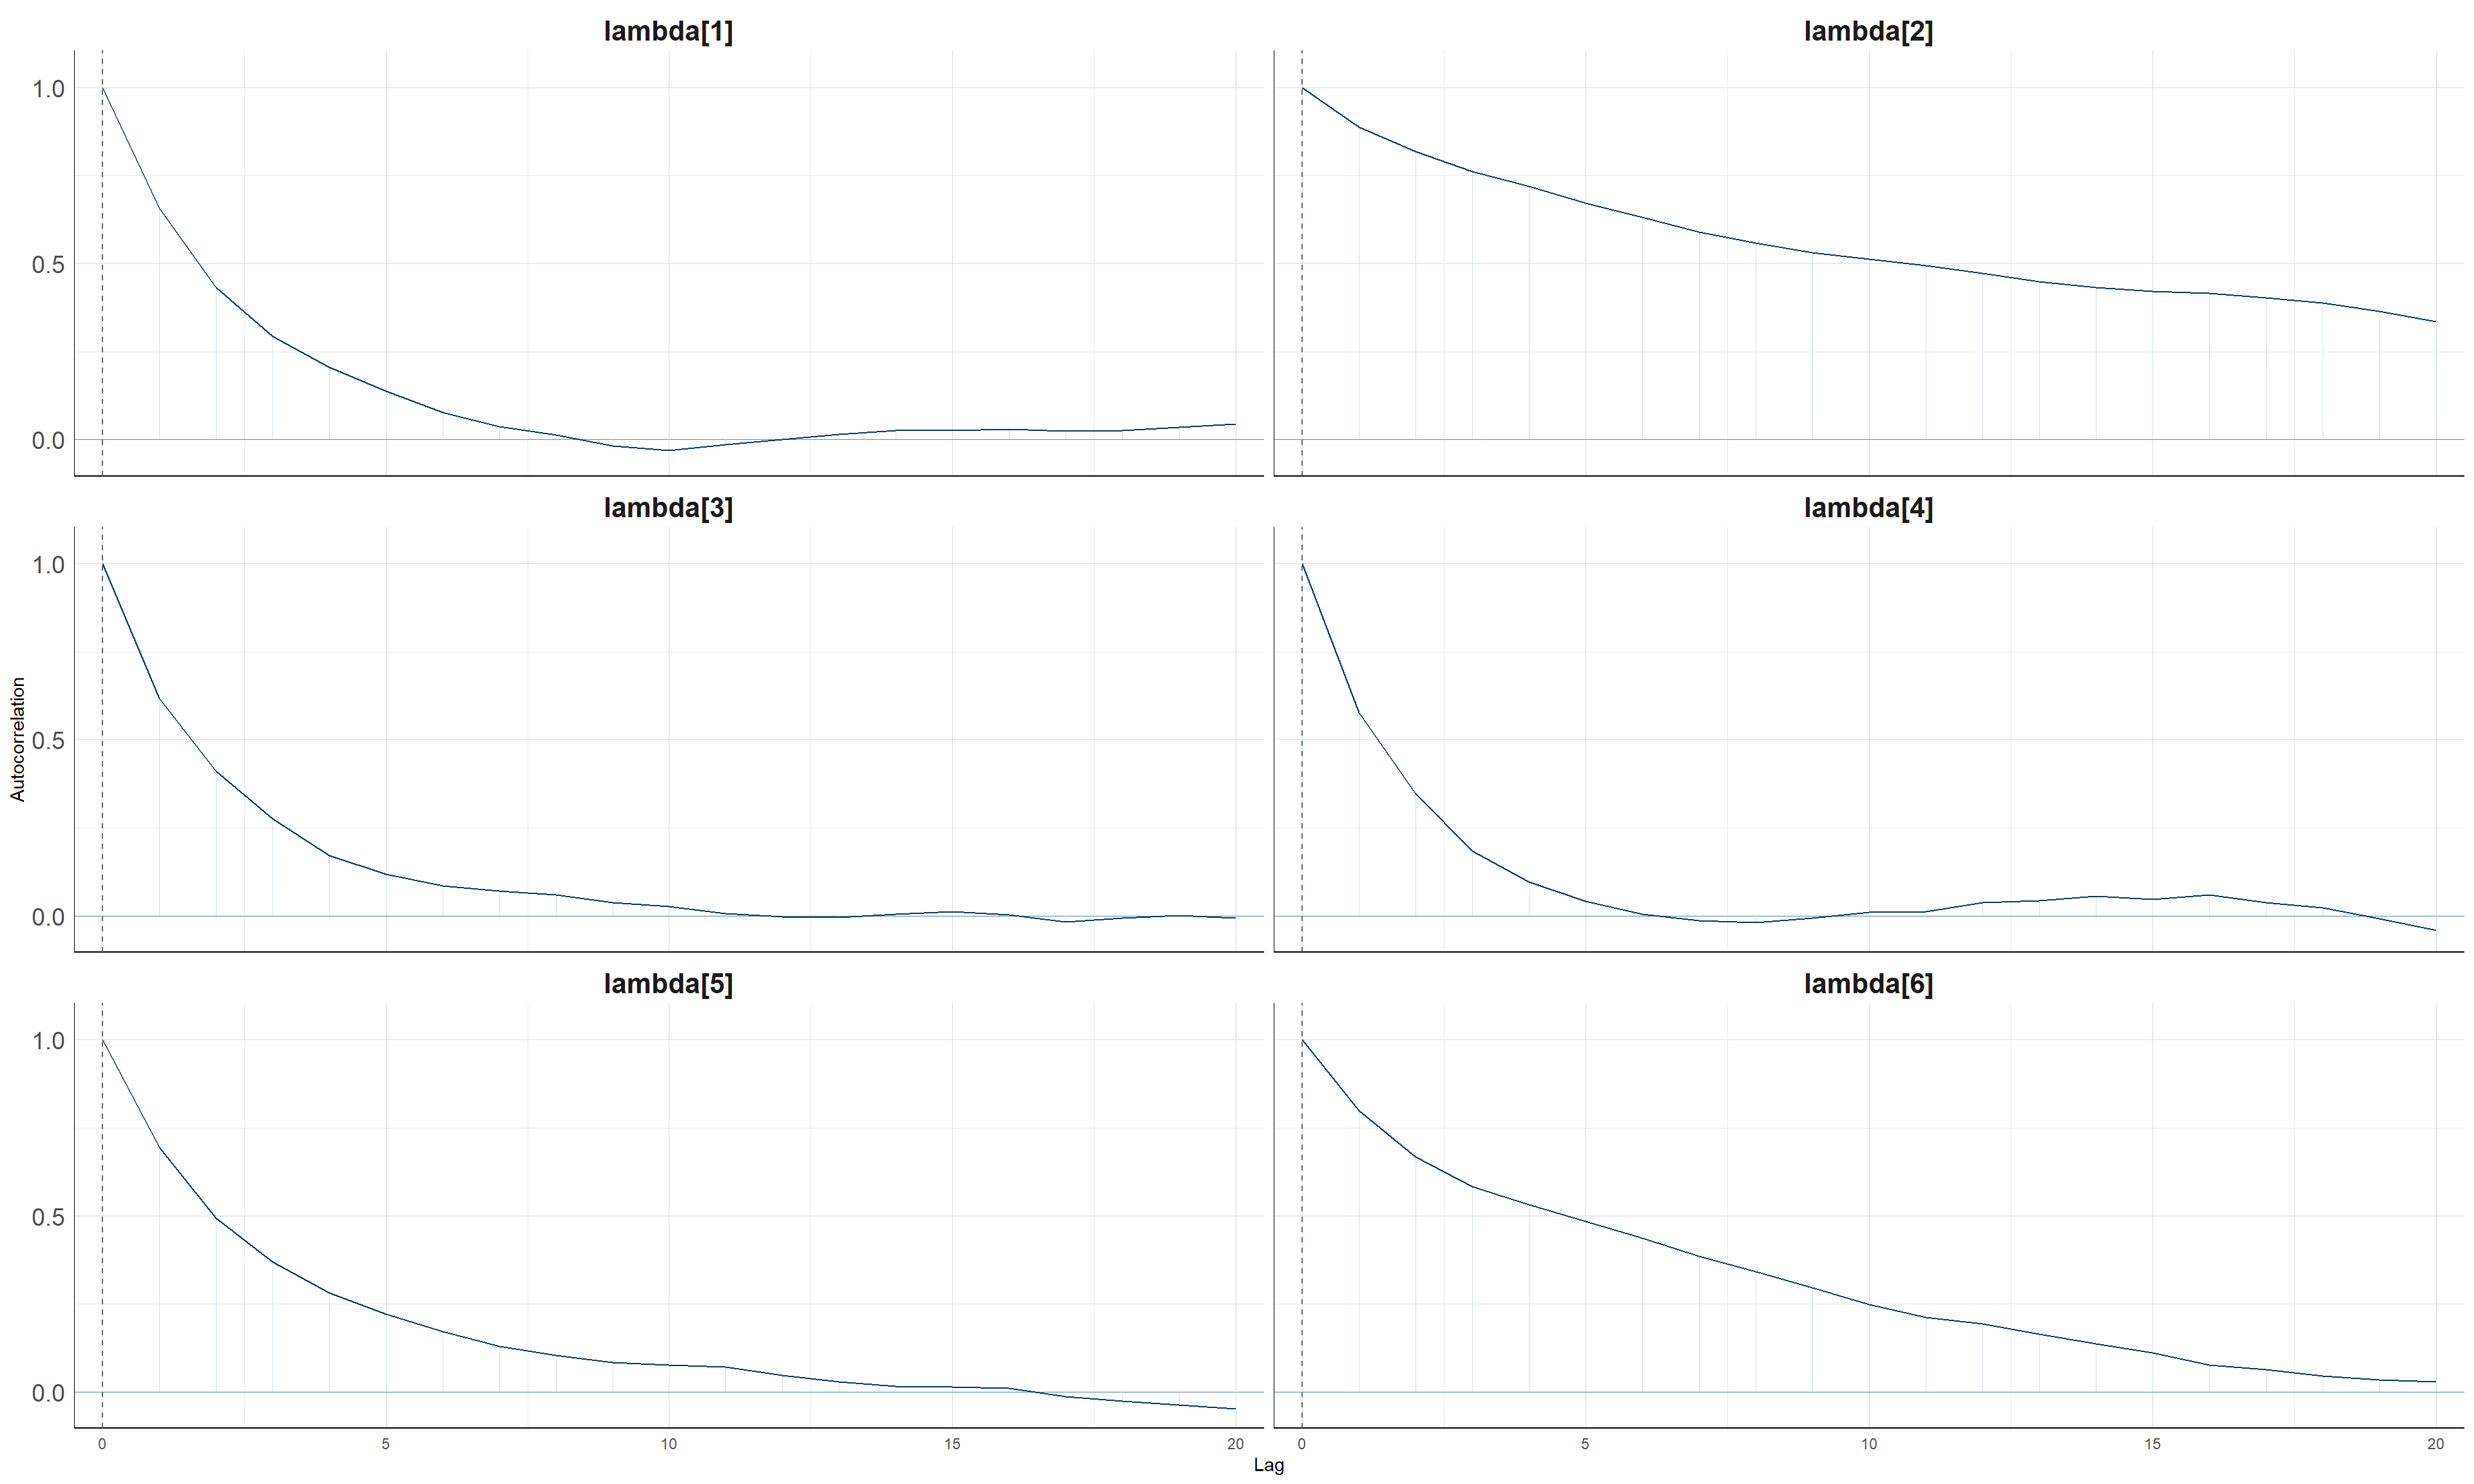
\includegraphics[width=\linewidth]{img/horseshoe_model/acf_lambda_chain1_1.png}
    \caption{Group 1.}
  \end{subfigure}\hfill
  \begin{subfigure}[t]{0.48\linewidth}
    \centering
    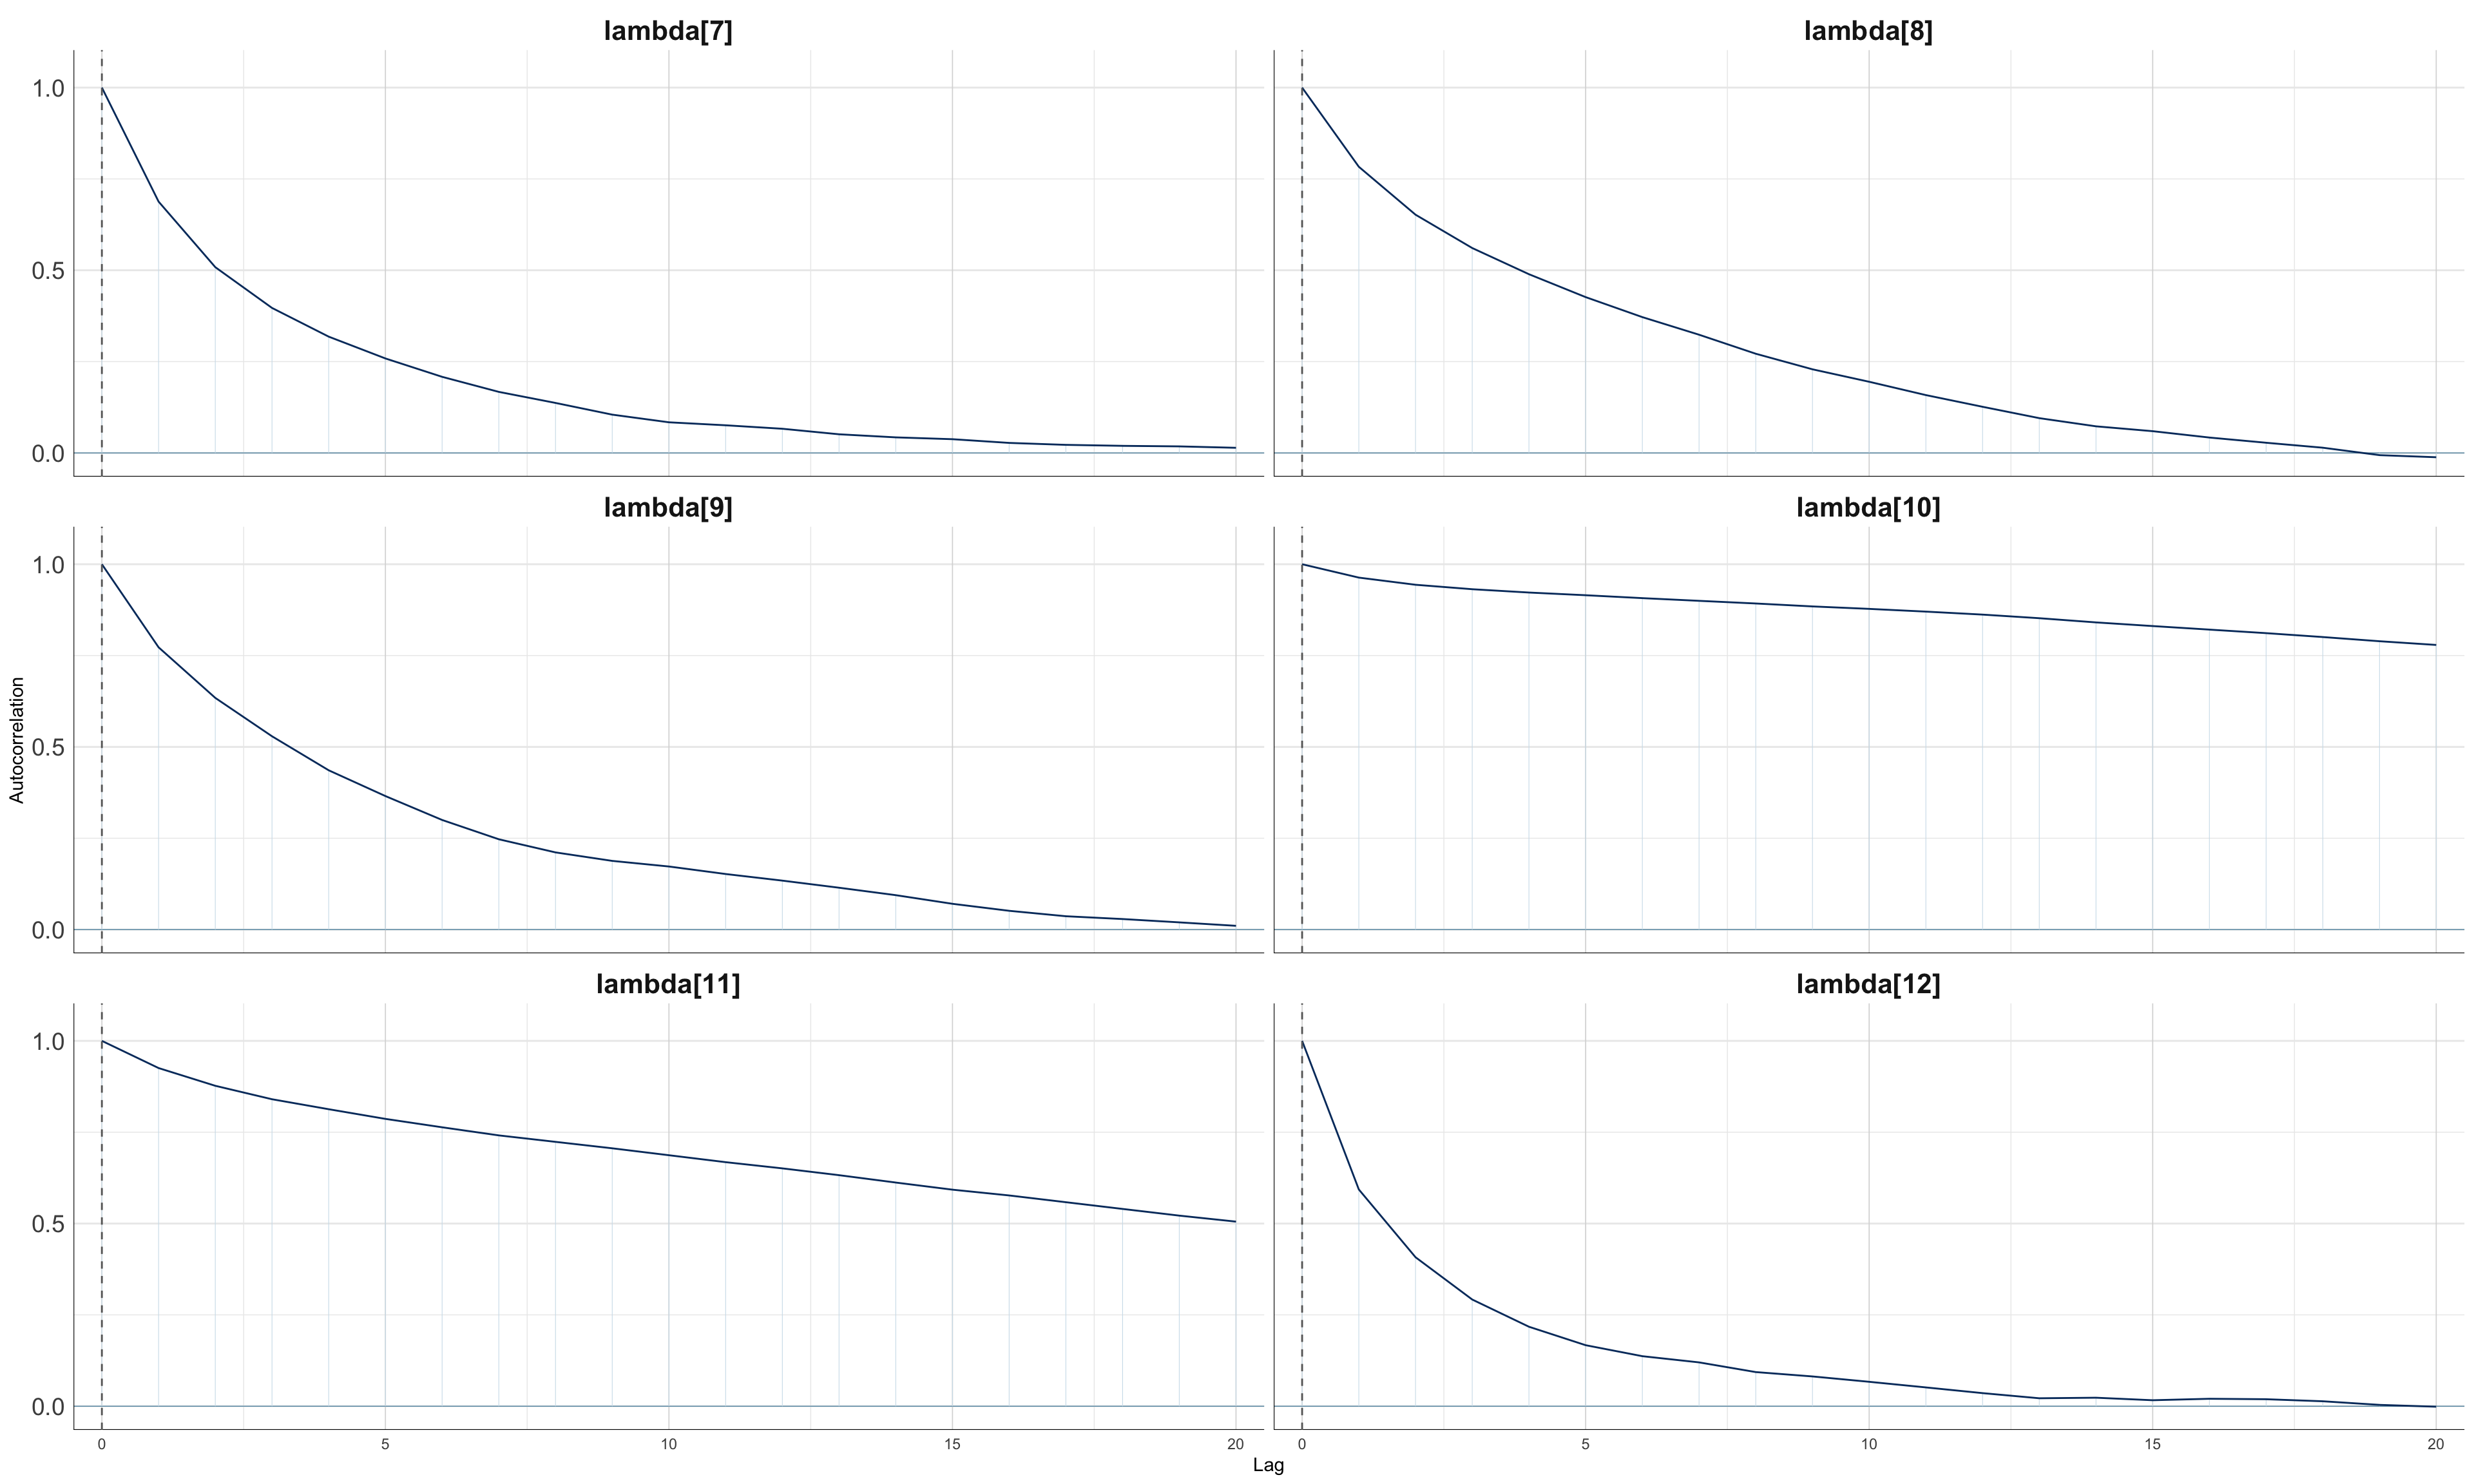
\includegraphics[width=\linewidth]{img/horseshoe_model/acf_lambda_chain1_2.png}
    \caption{Group 2.}
  \end{subfigure}\hfill
  \begin{subfigure}[t]{0.48\linewidth}
    \centering
    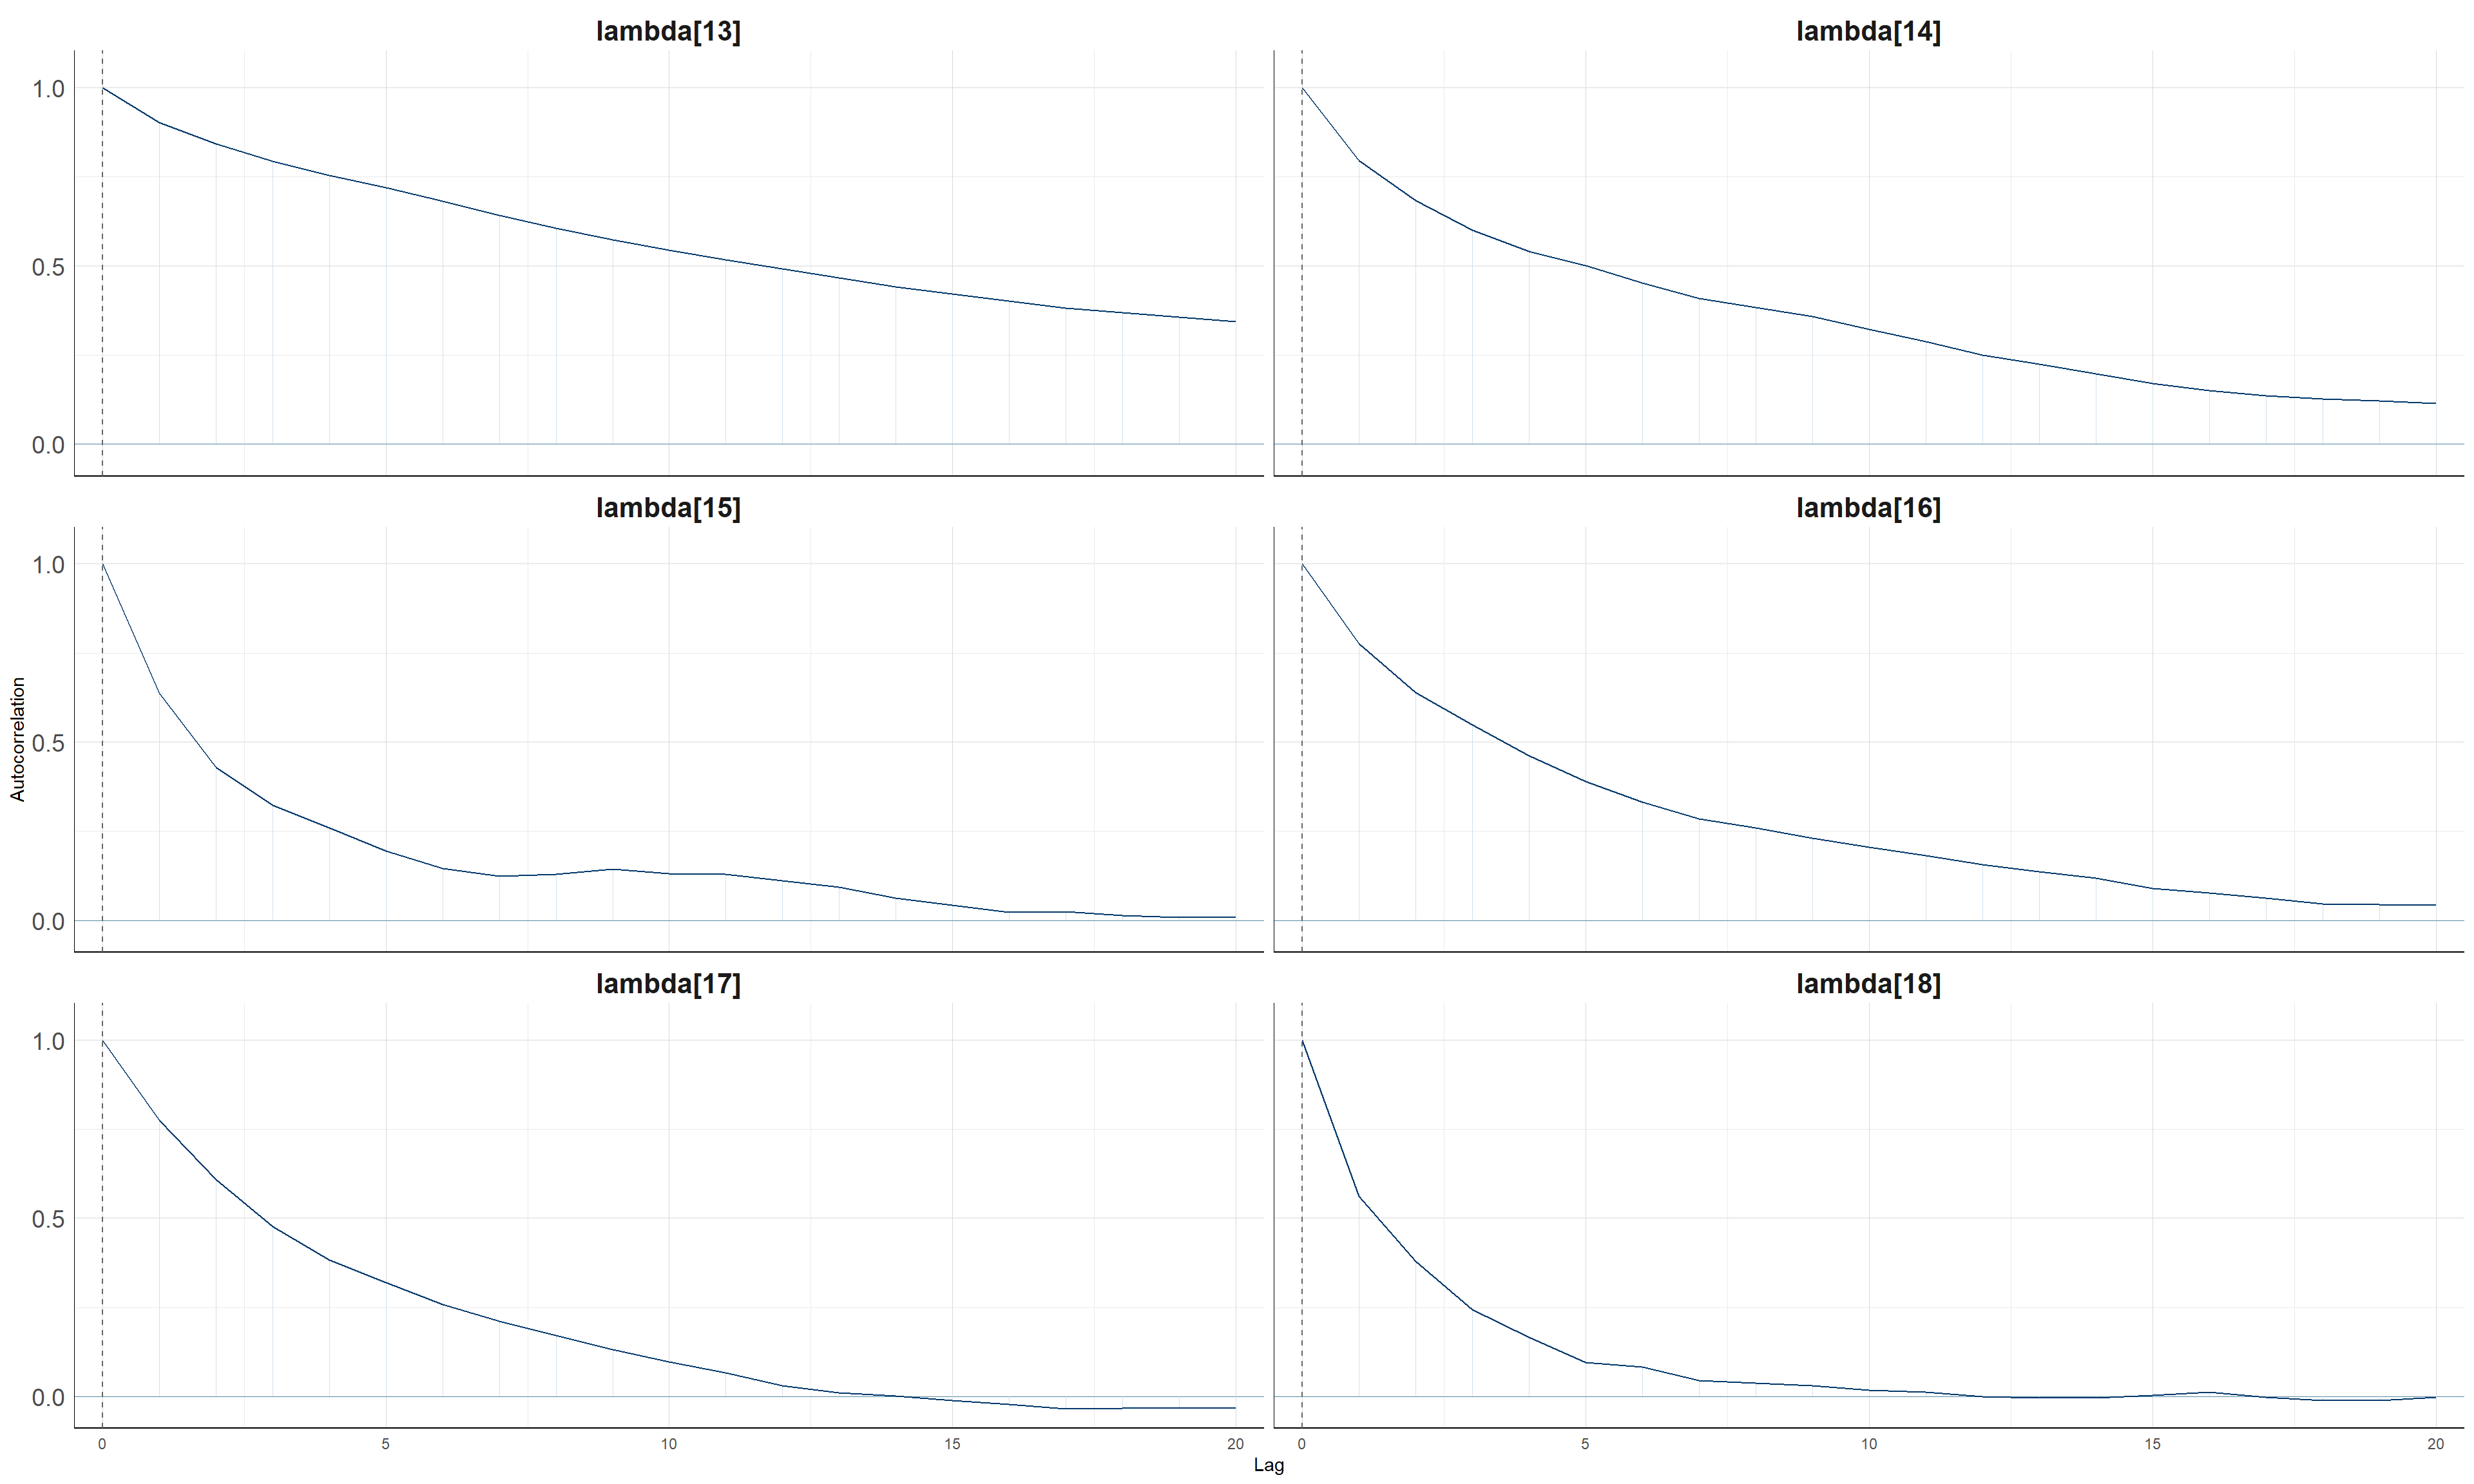
\includegraphics[width=\linewidth]{img/horseshoe_model/acf_lambda_chain1_3.png}
    \caption{Group 3.}
  \end{subfigure}\hfill
  \begin{subfigure}[t]{0.48\linewidth}
    \centering
    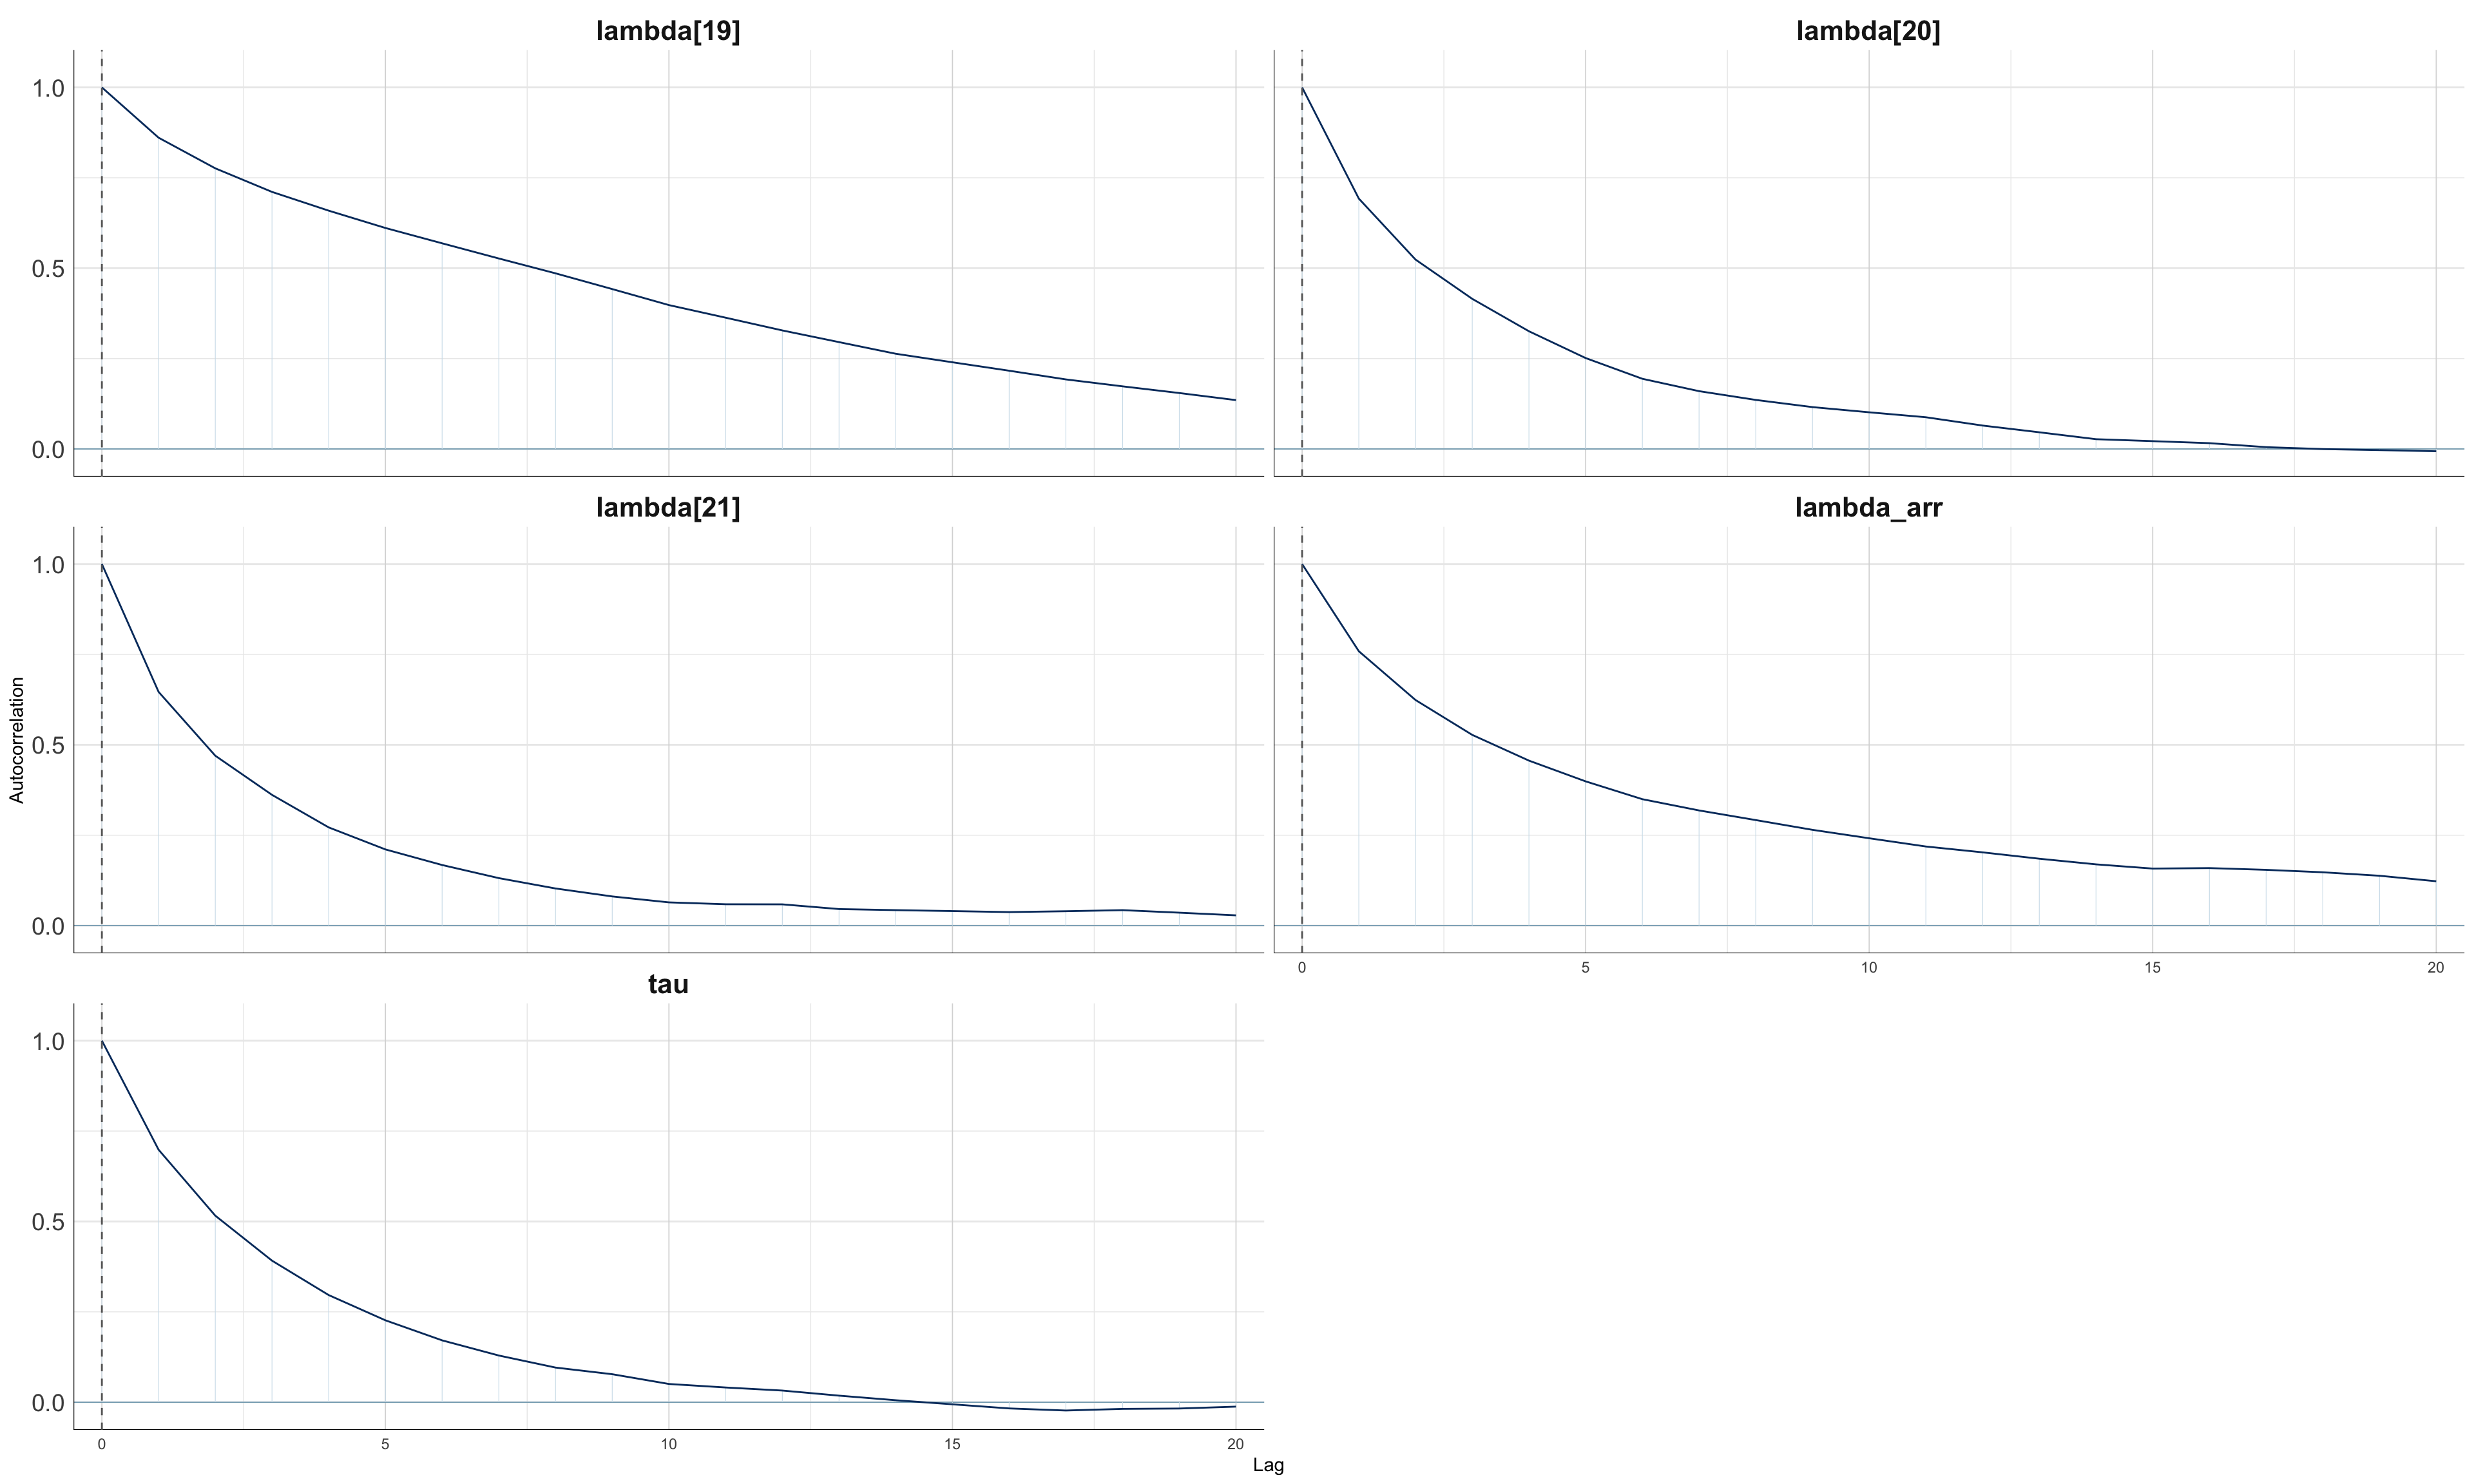
\includegraphics[width=\linewidth]{img/horseshoe_model/acf_lambda_chain1_4.png}
    \caption{Group 4.}
  \end{subfigure}\hfill
  \caption{Autocorrelation of the scales $\lambda_j$, chain 1.}
  \label{fig:hs_acf_lambda_1}
\end{figure}

\begin{figure}[htbp]
  \centering
  \begin{subfigure}[t]{0.48\linewidth}
    \centering
    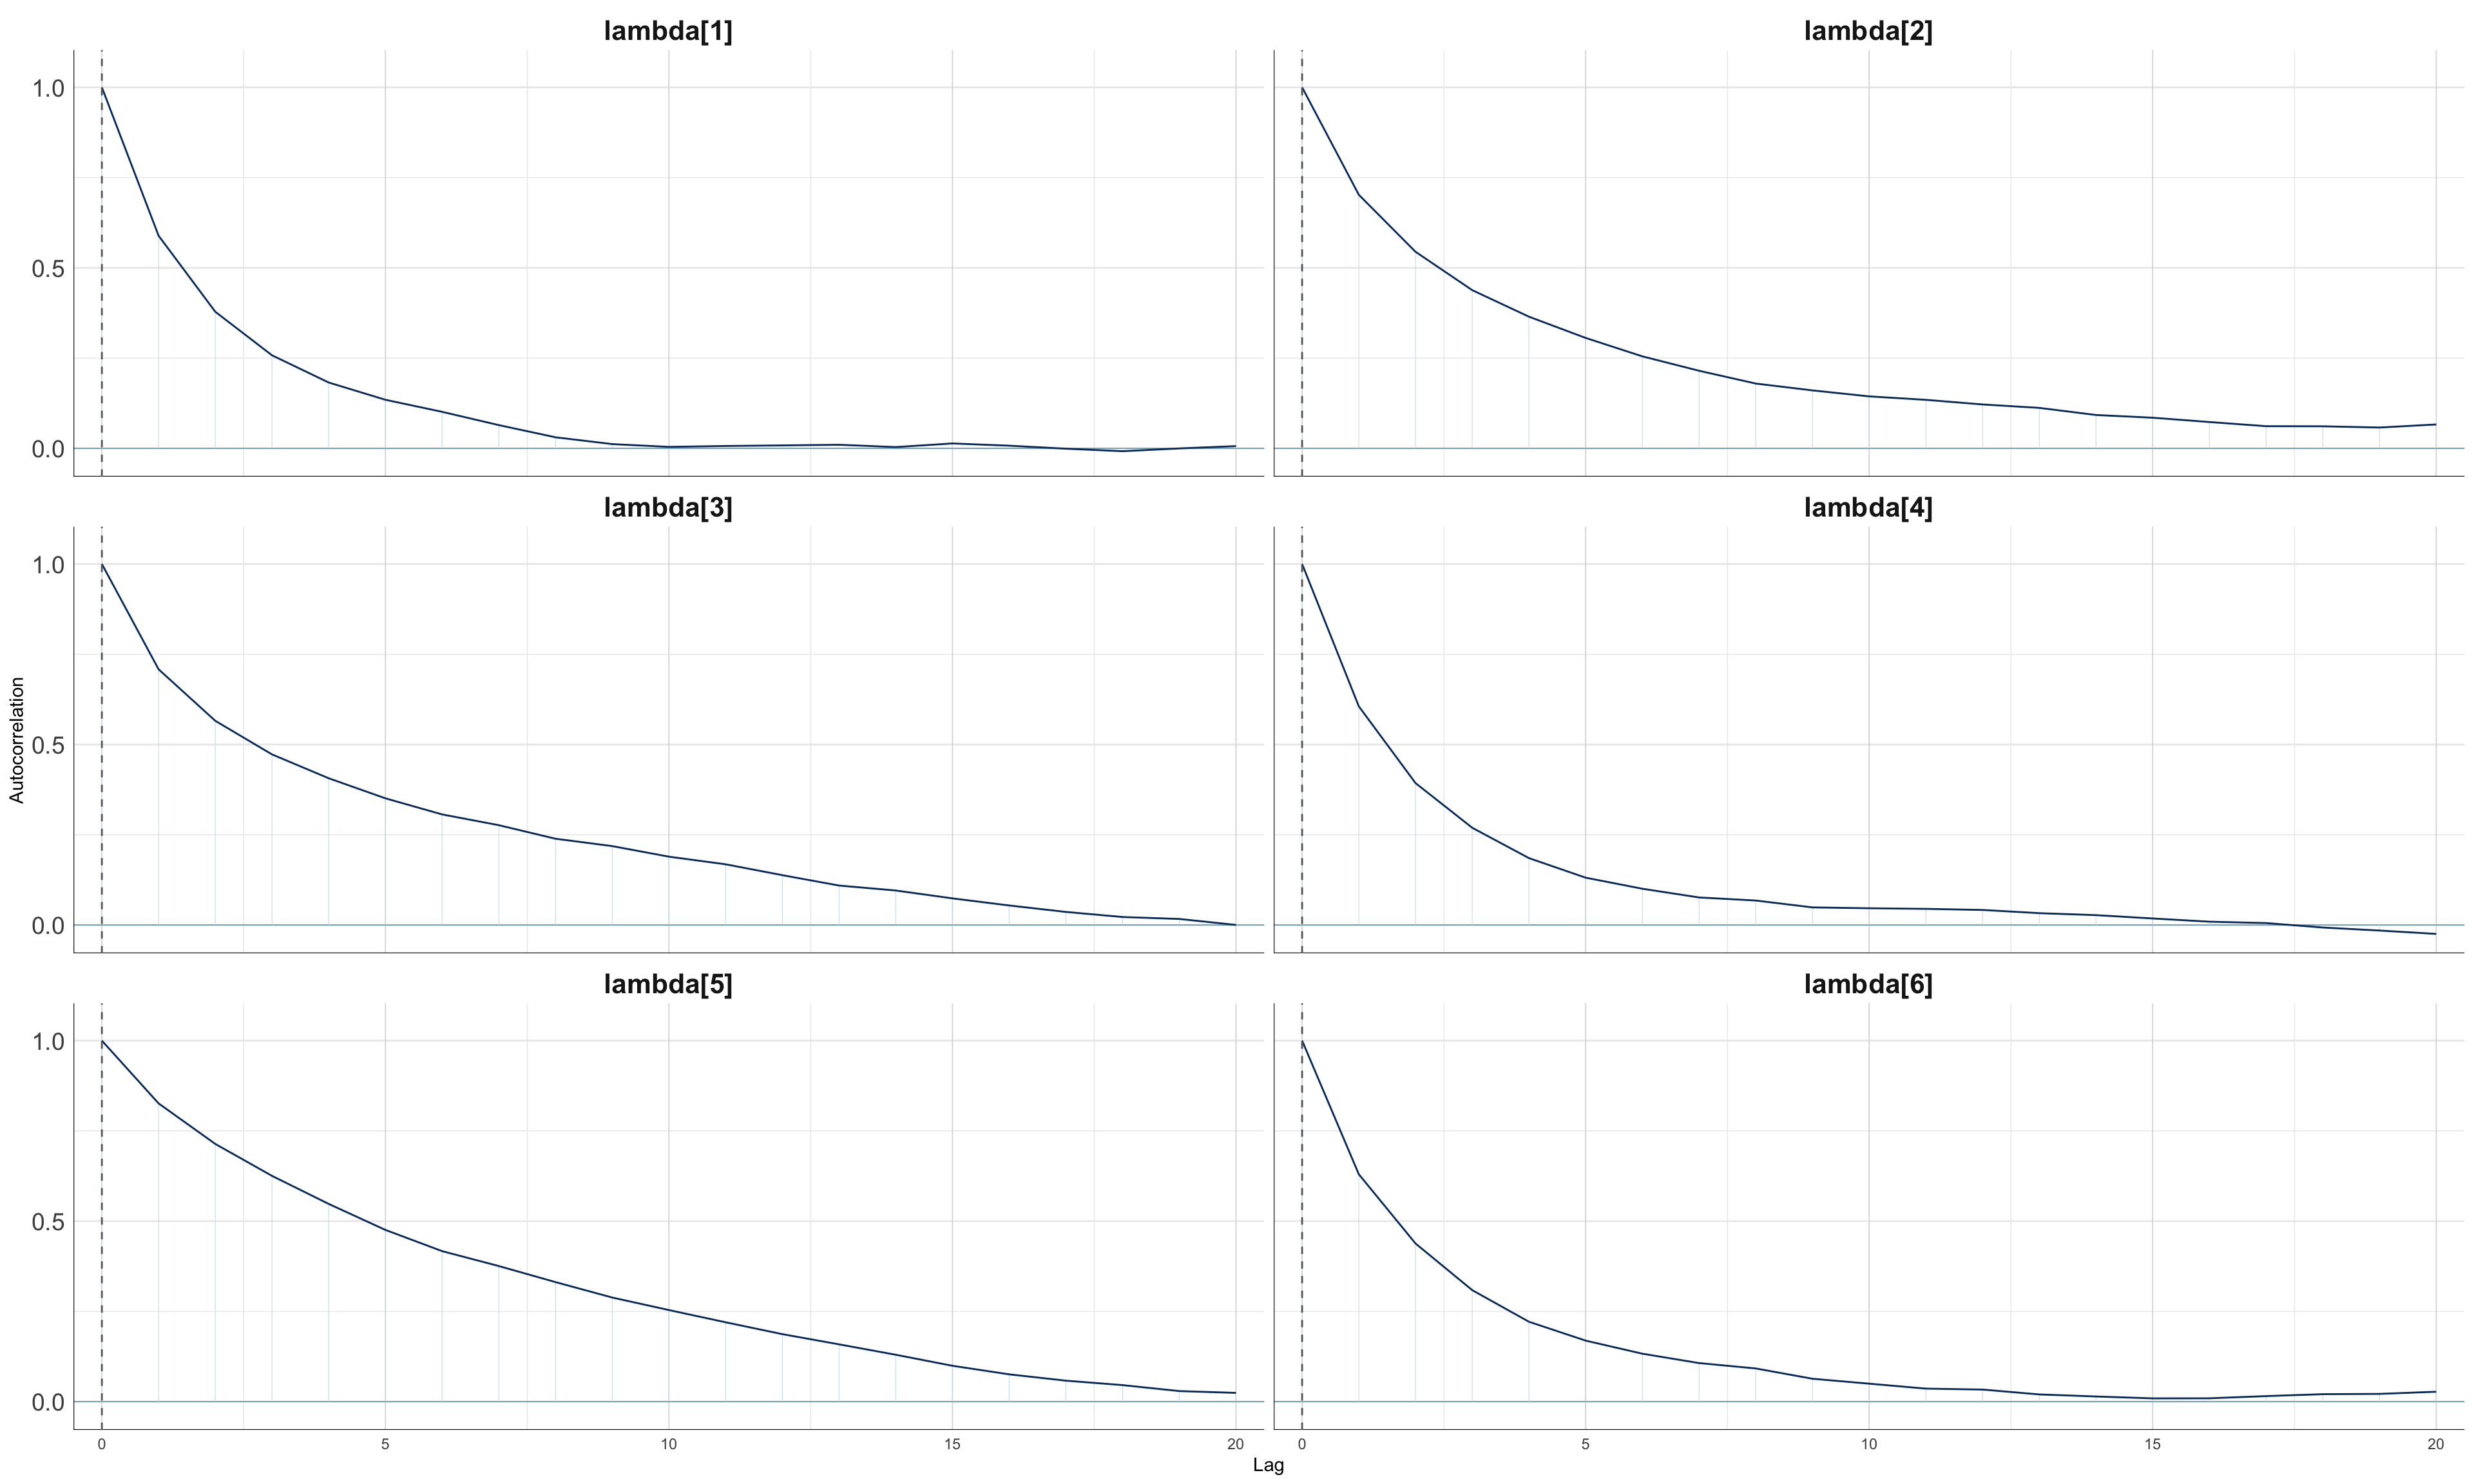
\includegraphics[width=\linewidth]{img/horseshoe_model/acf_lambda_chain2_1.png}
    \caption{Group 1.}
  \end{subfigure}\hfill
  \begin{subfigure}[t]{0.48\linewidth}
    \centering
    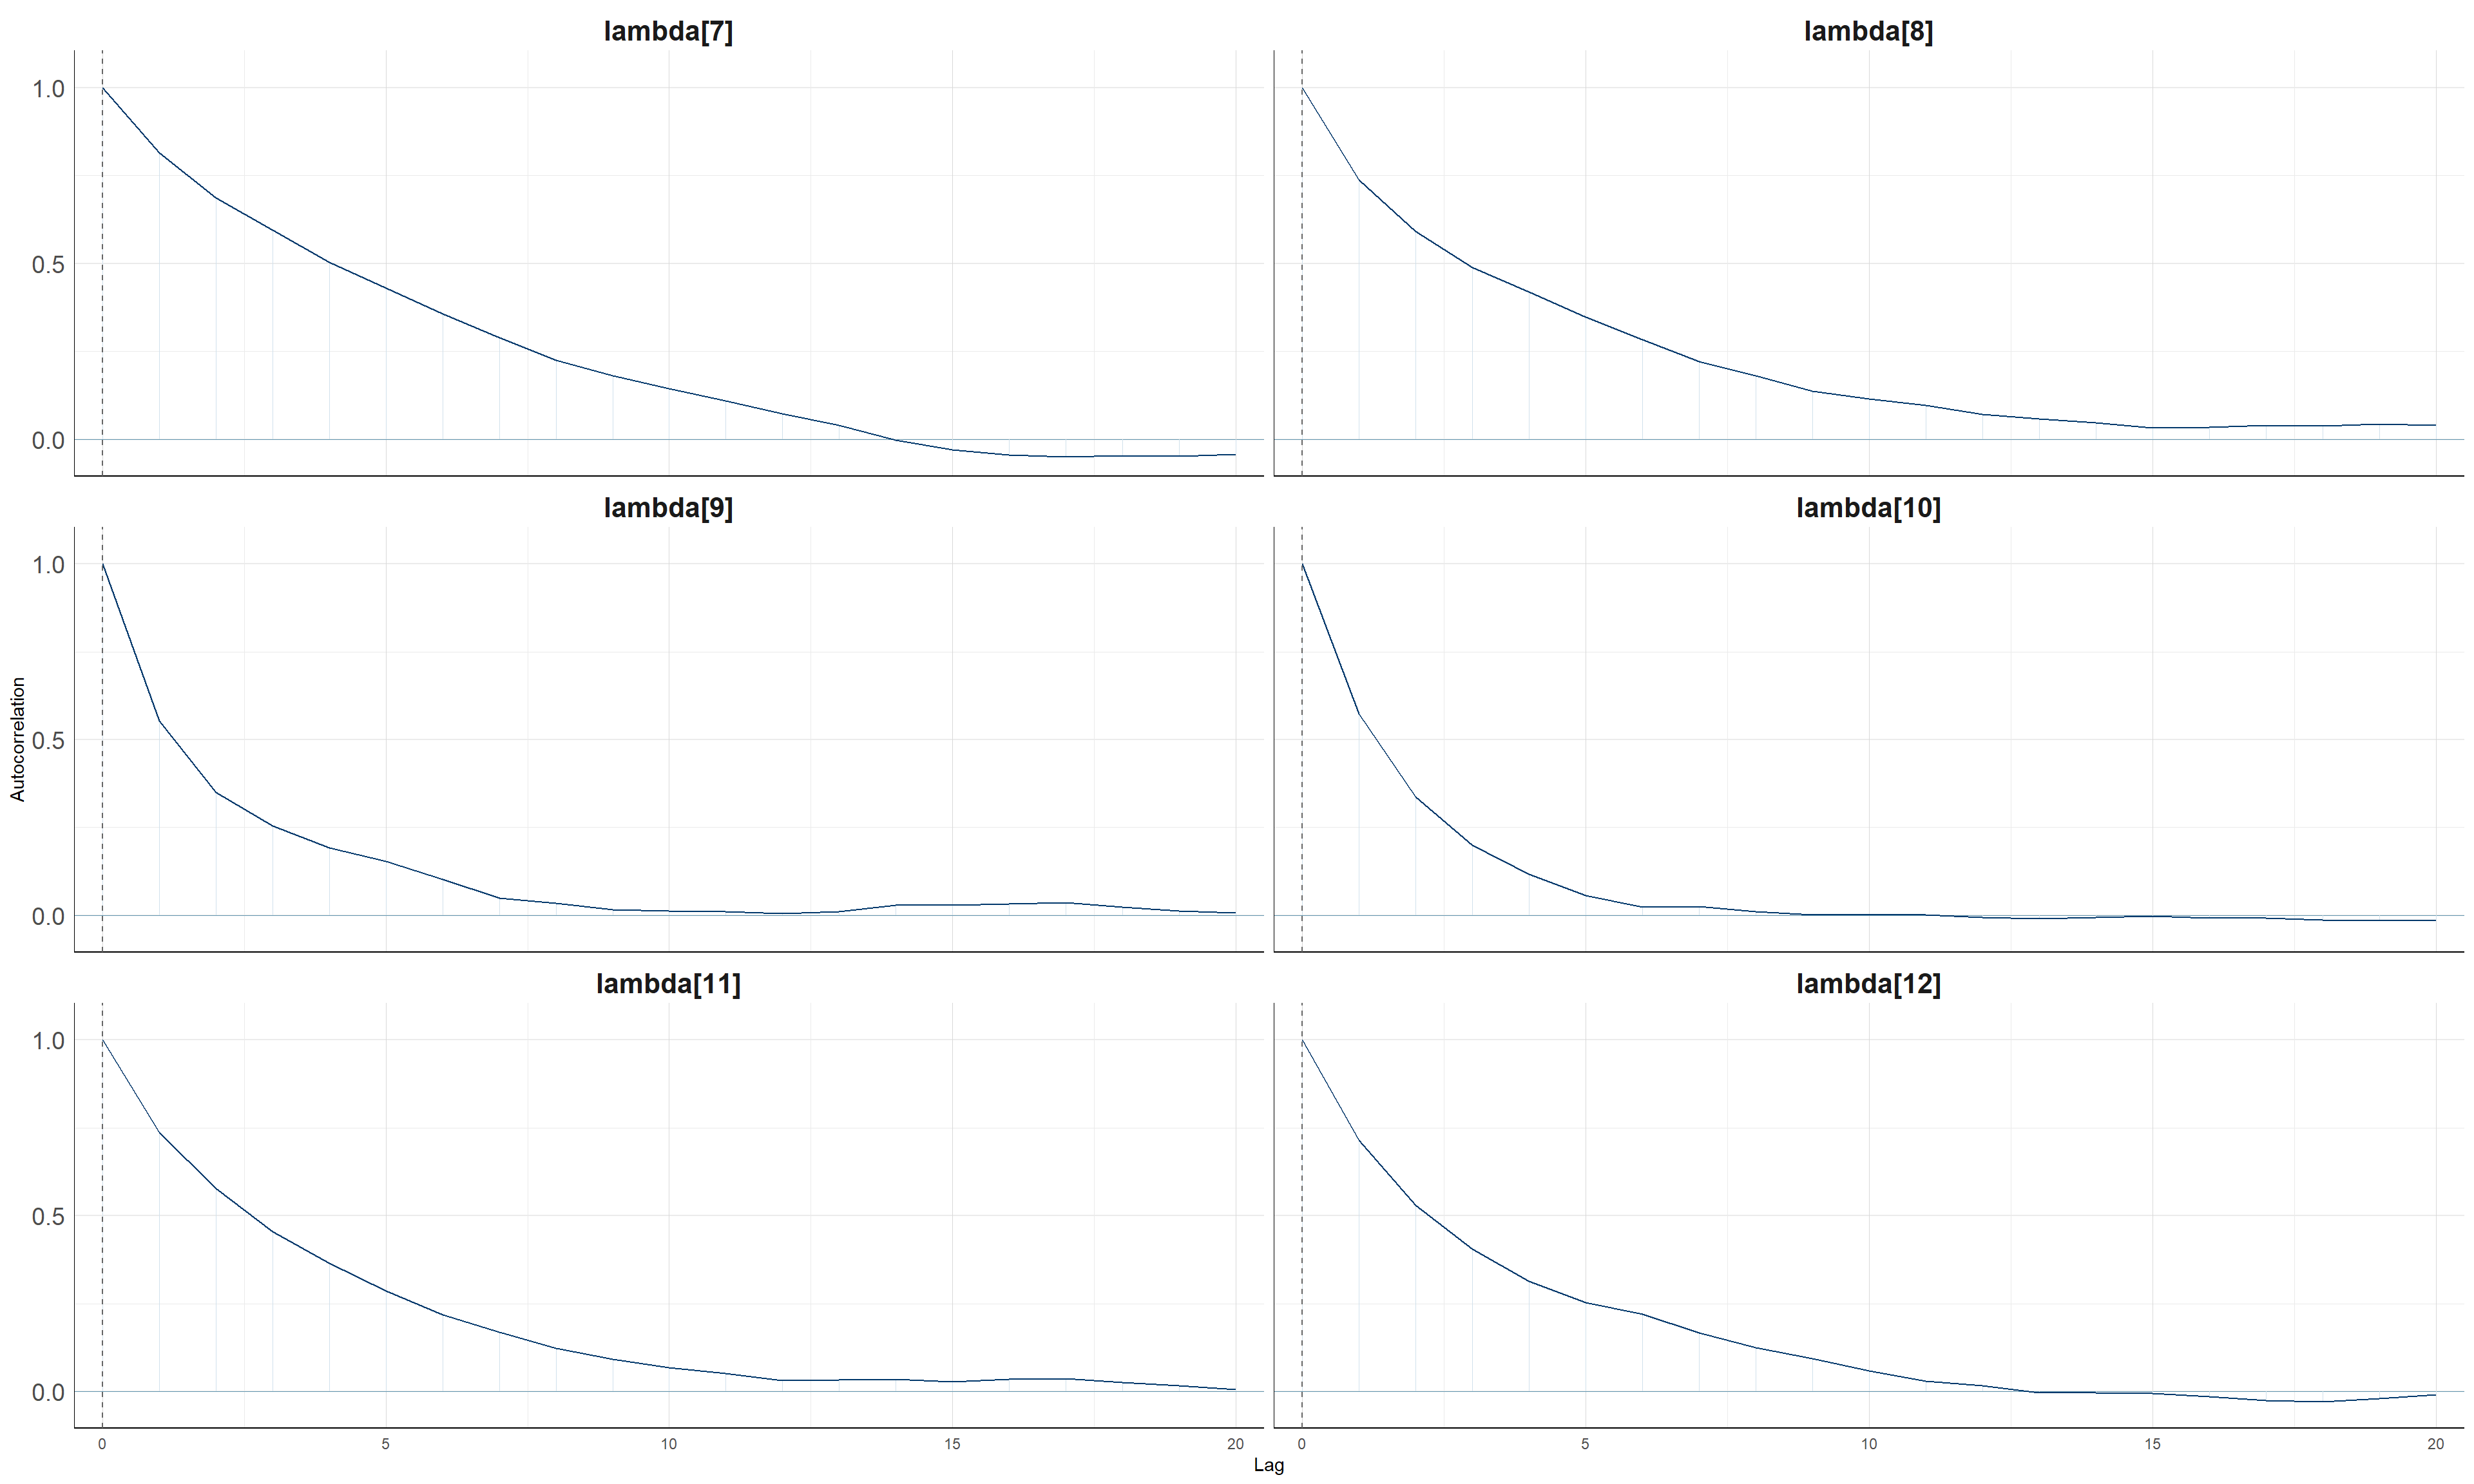
\includegraphics[width=\linewidth]{img/horseshoe_model/acf_lambda_chain2_2.png}
    \caption{Group 2.}
  \end{subfigure}\hfill
  \begin{subfigure}[t]{0.48\linewidth}
    \centering
    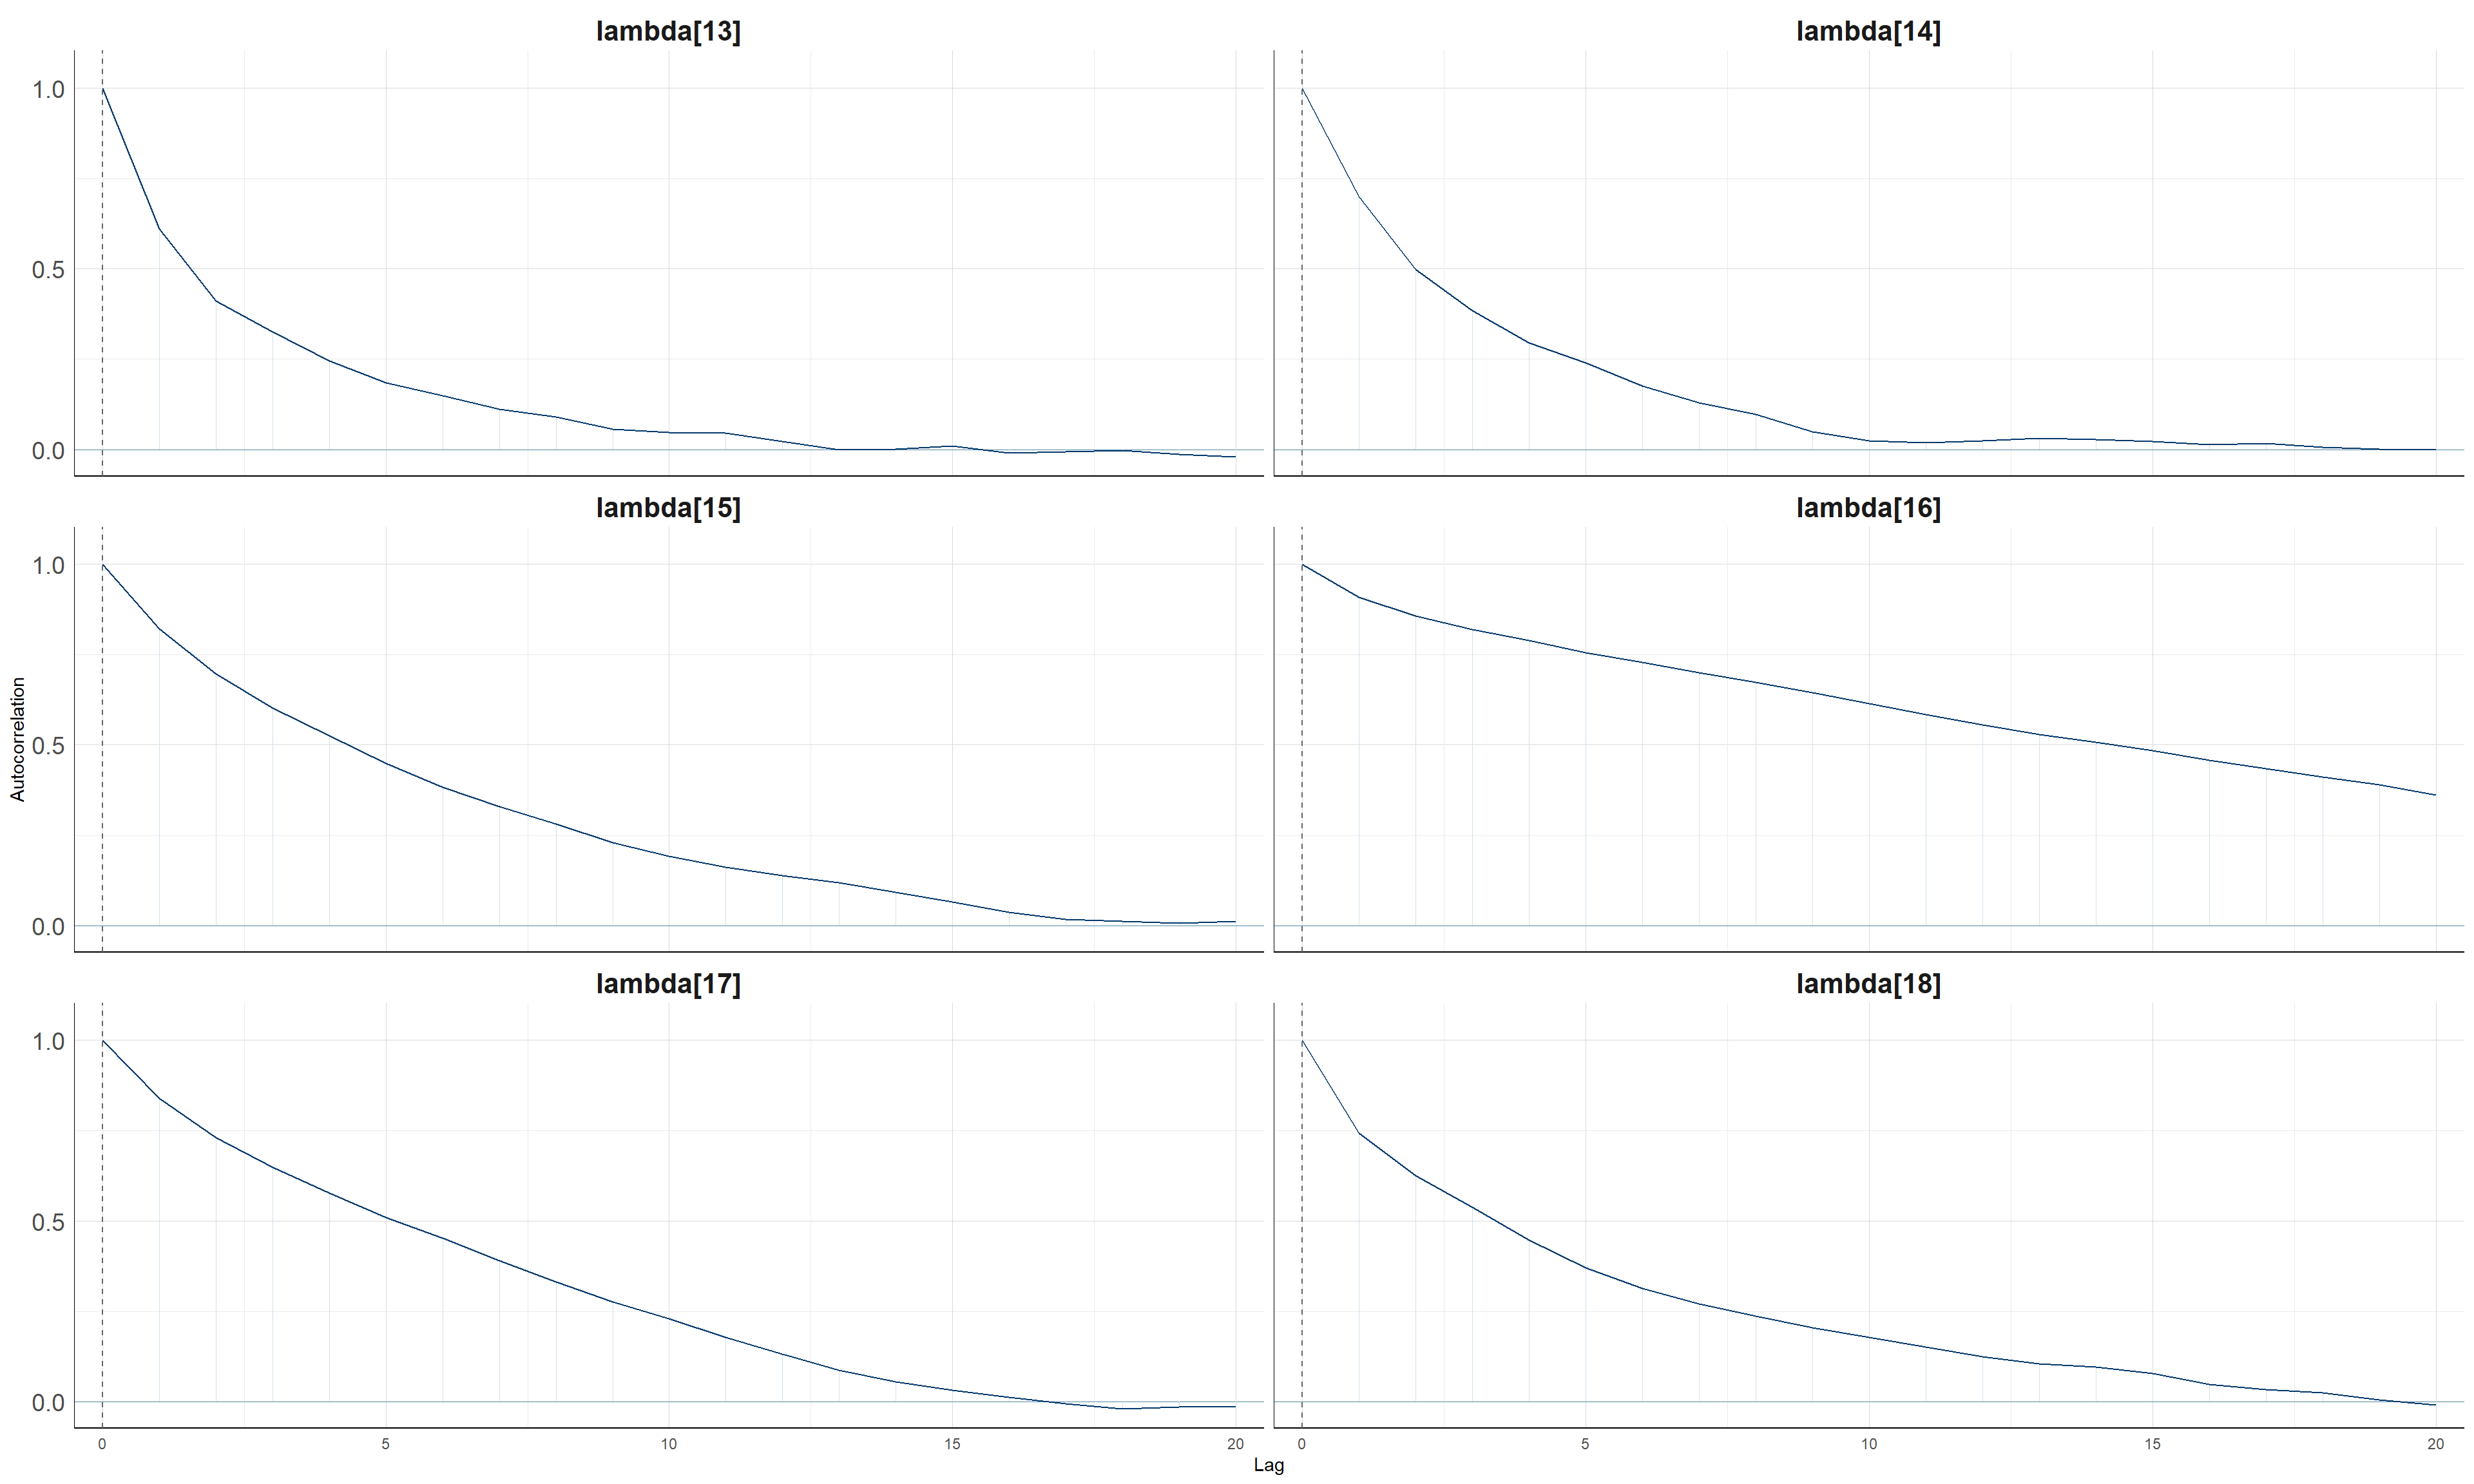
\includegraphics[width=\linewidth]{img/horseshoe_model/acf_lambda_chain2_3.png}
    \caption{Group 3.}
  \end{subfigure}\hfill
  \begin{subfigure}[t]{0.48\linewidth}
    \centering
    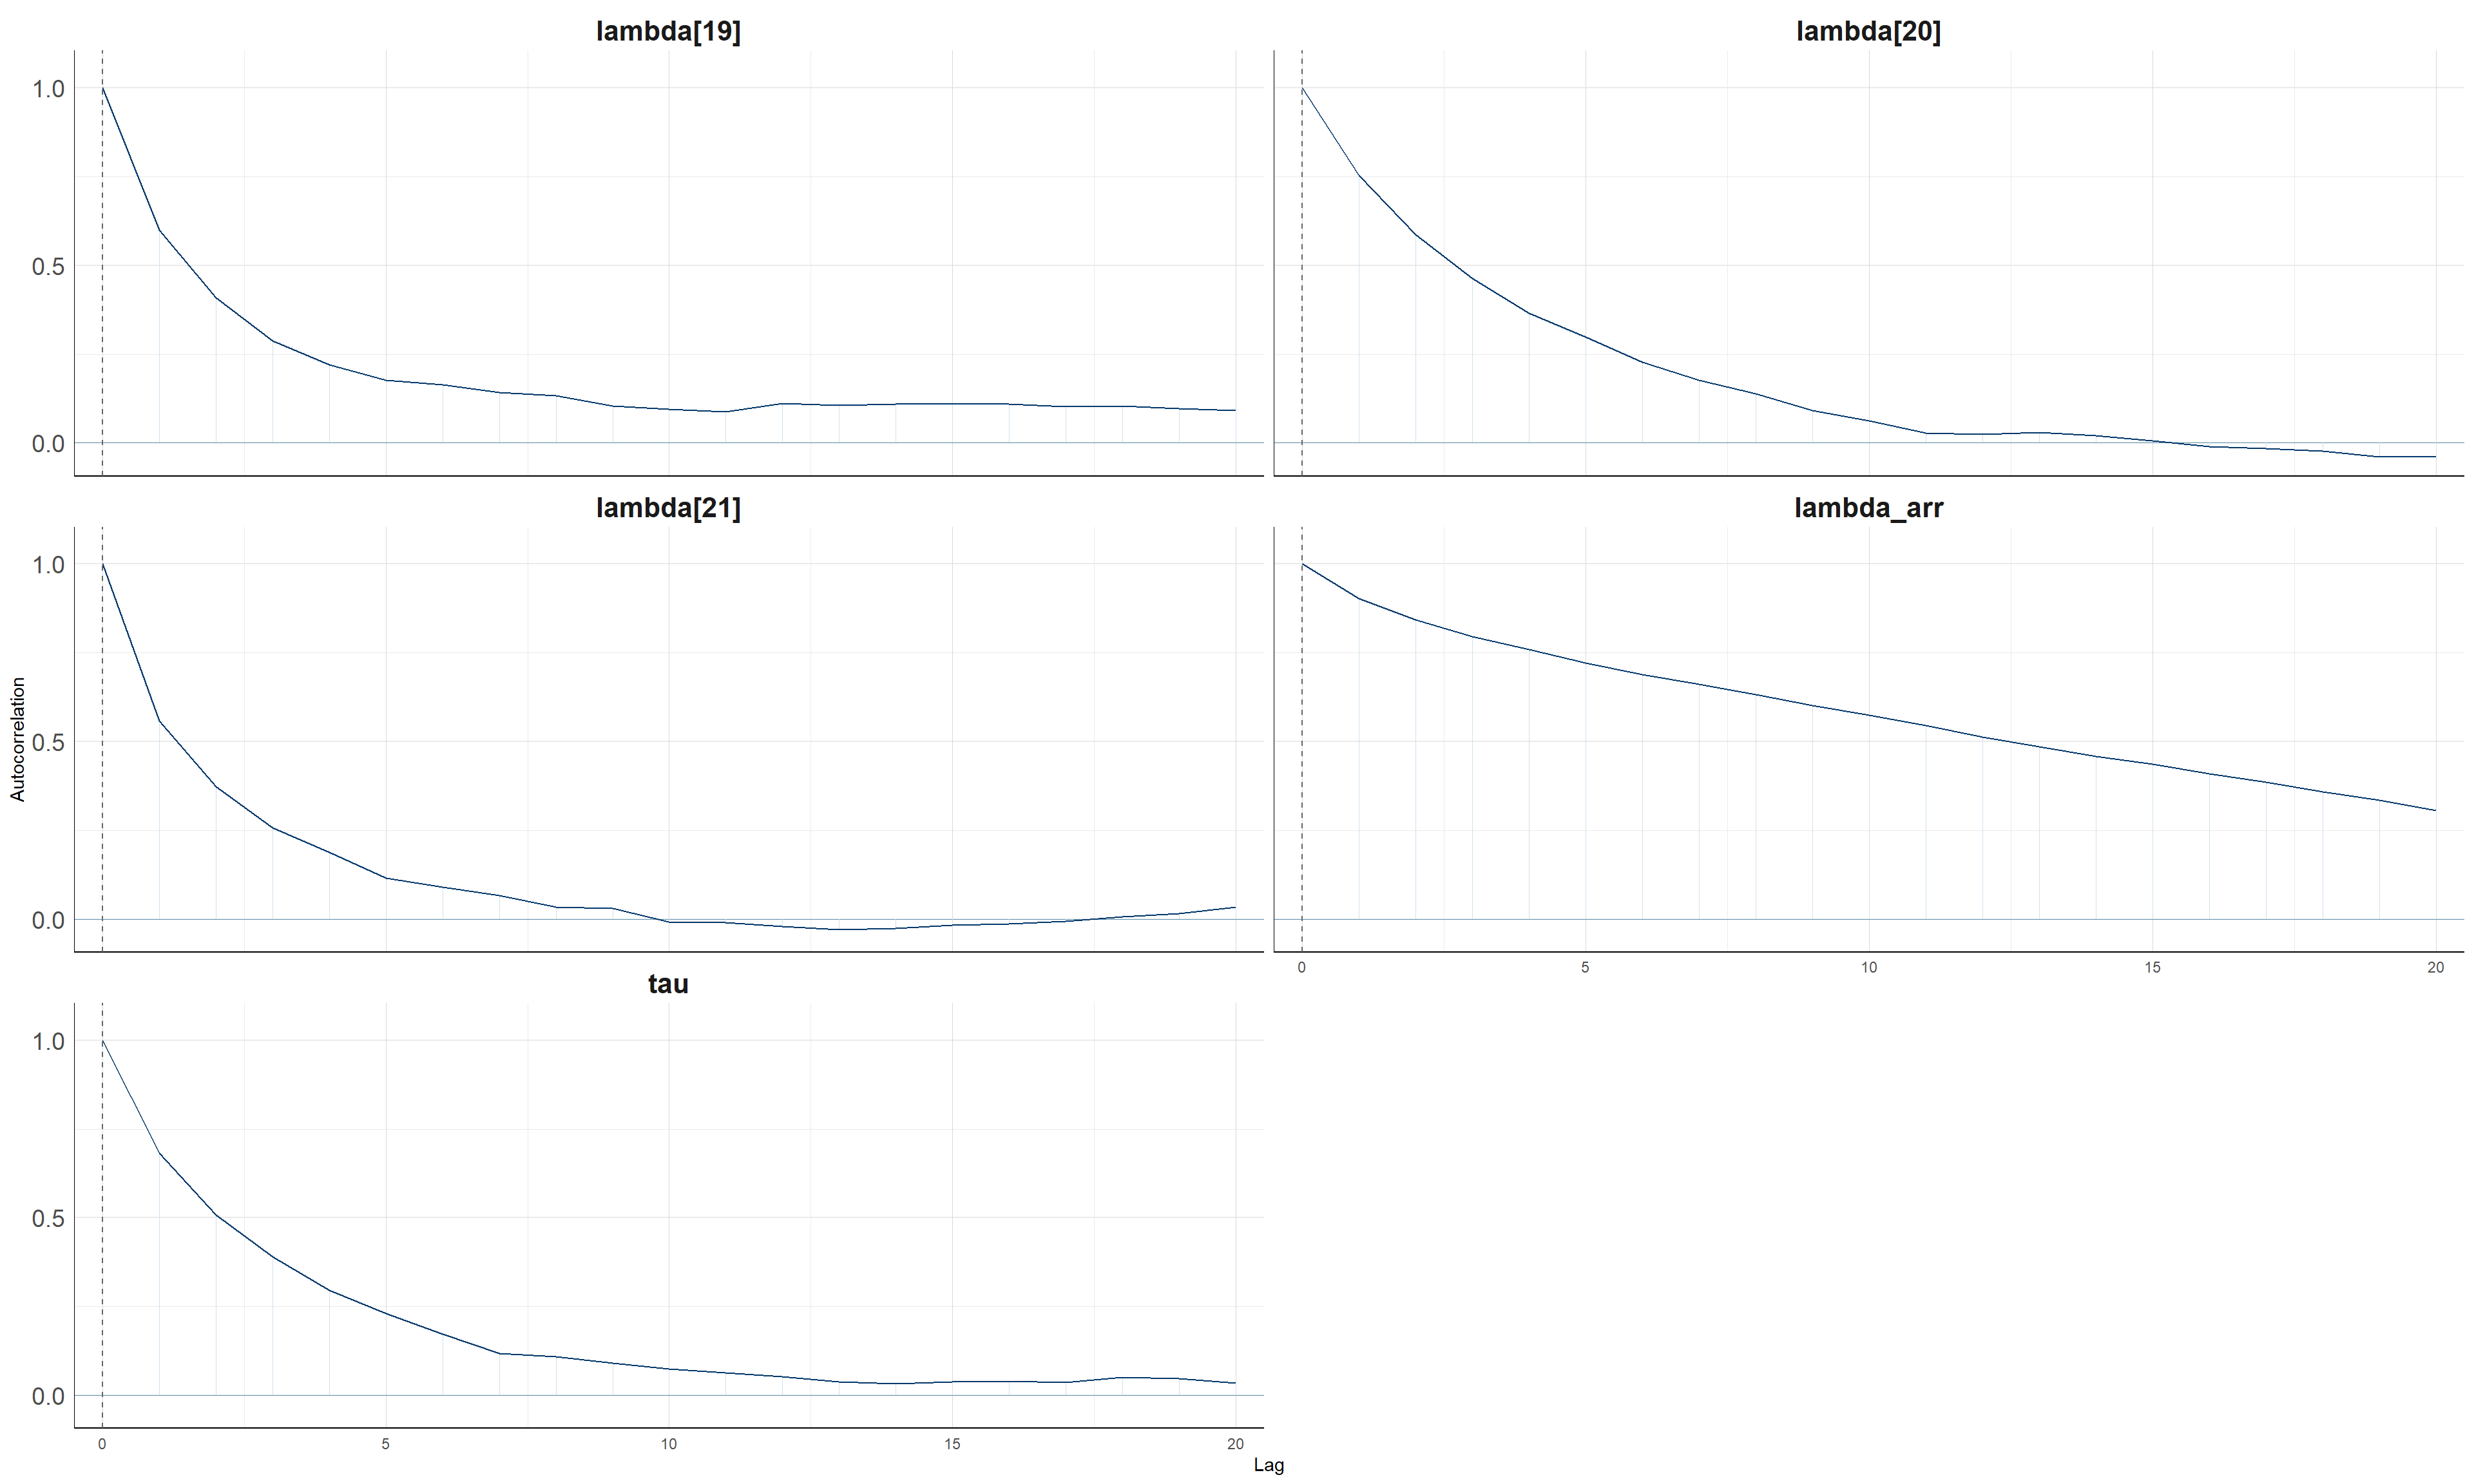
\includegraphics[width=\linewidth]{img/horseshoe_model/acf_lambda_chain2_4.png}
    \caption{Group 4.}
  \end{subfigure}\hfill
  \caption{Autocorrelation of the scales $\lambda_j$, chain 2.}
  \label{fig:hs_acf_lambda_2}
\end{figure}

\begin{figure}[htbp]
  \centering
  \begin{subfigure}[t]{0.48\linewidth}
    \centering
    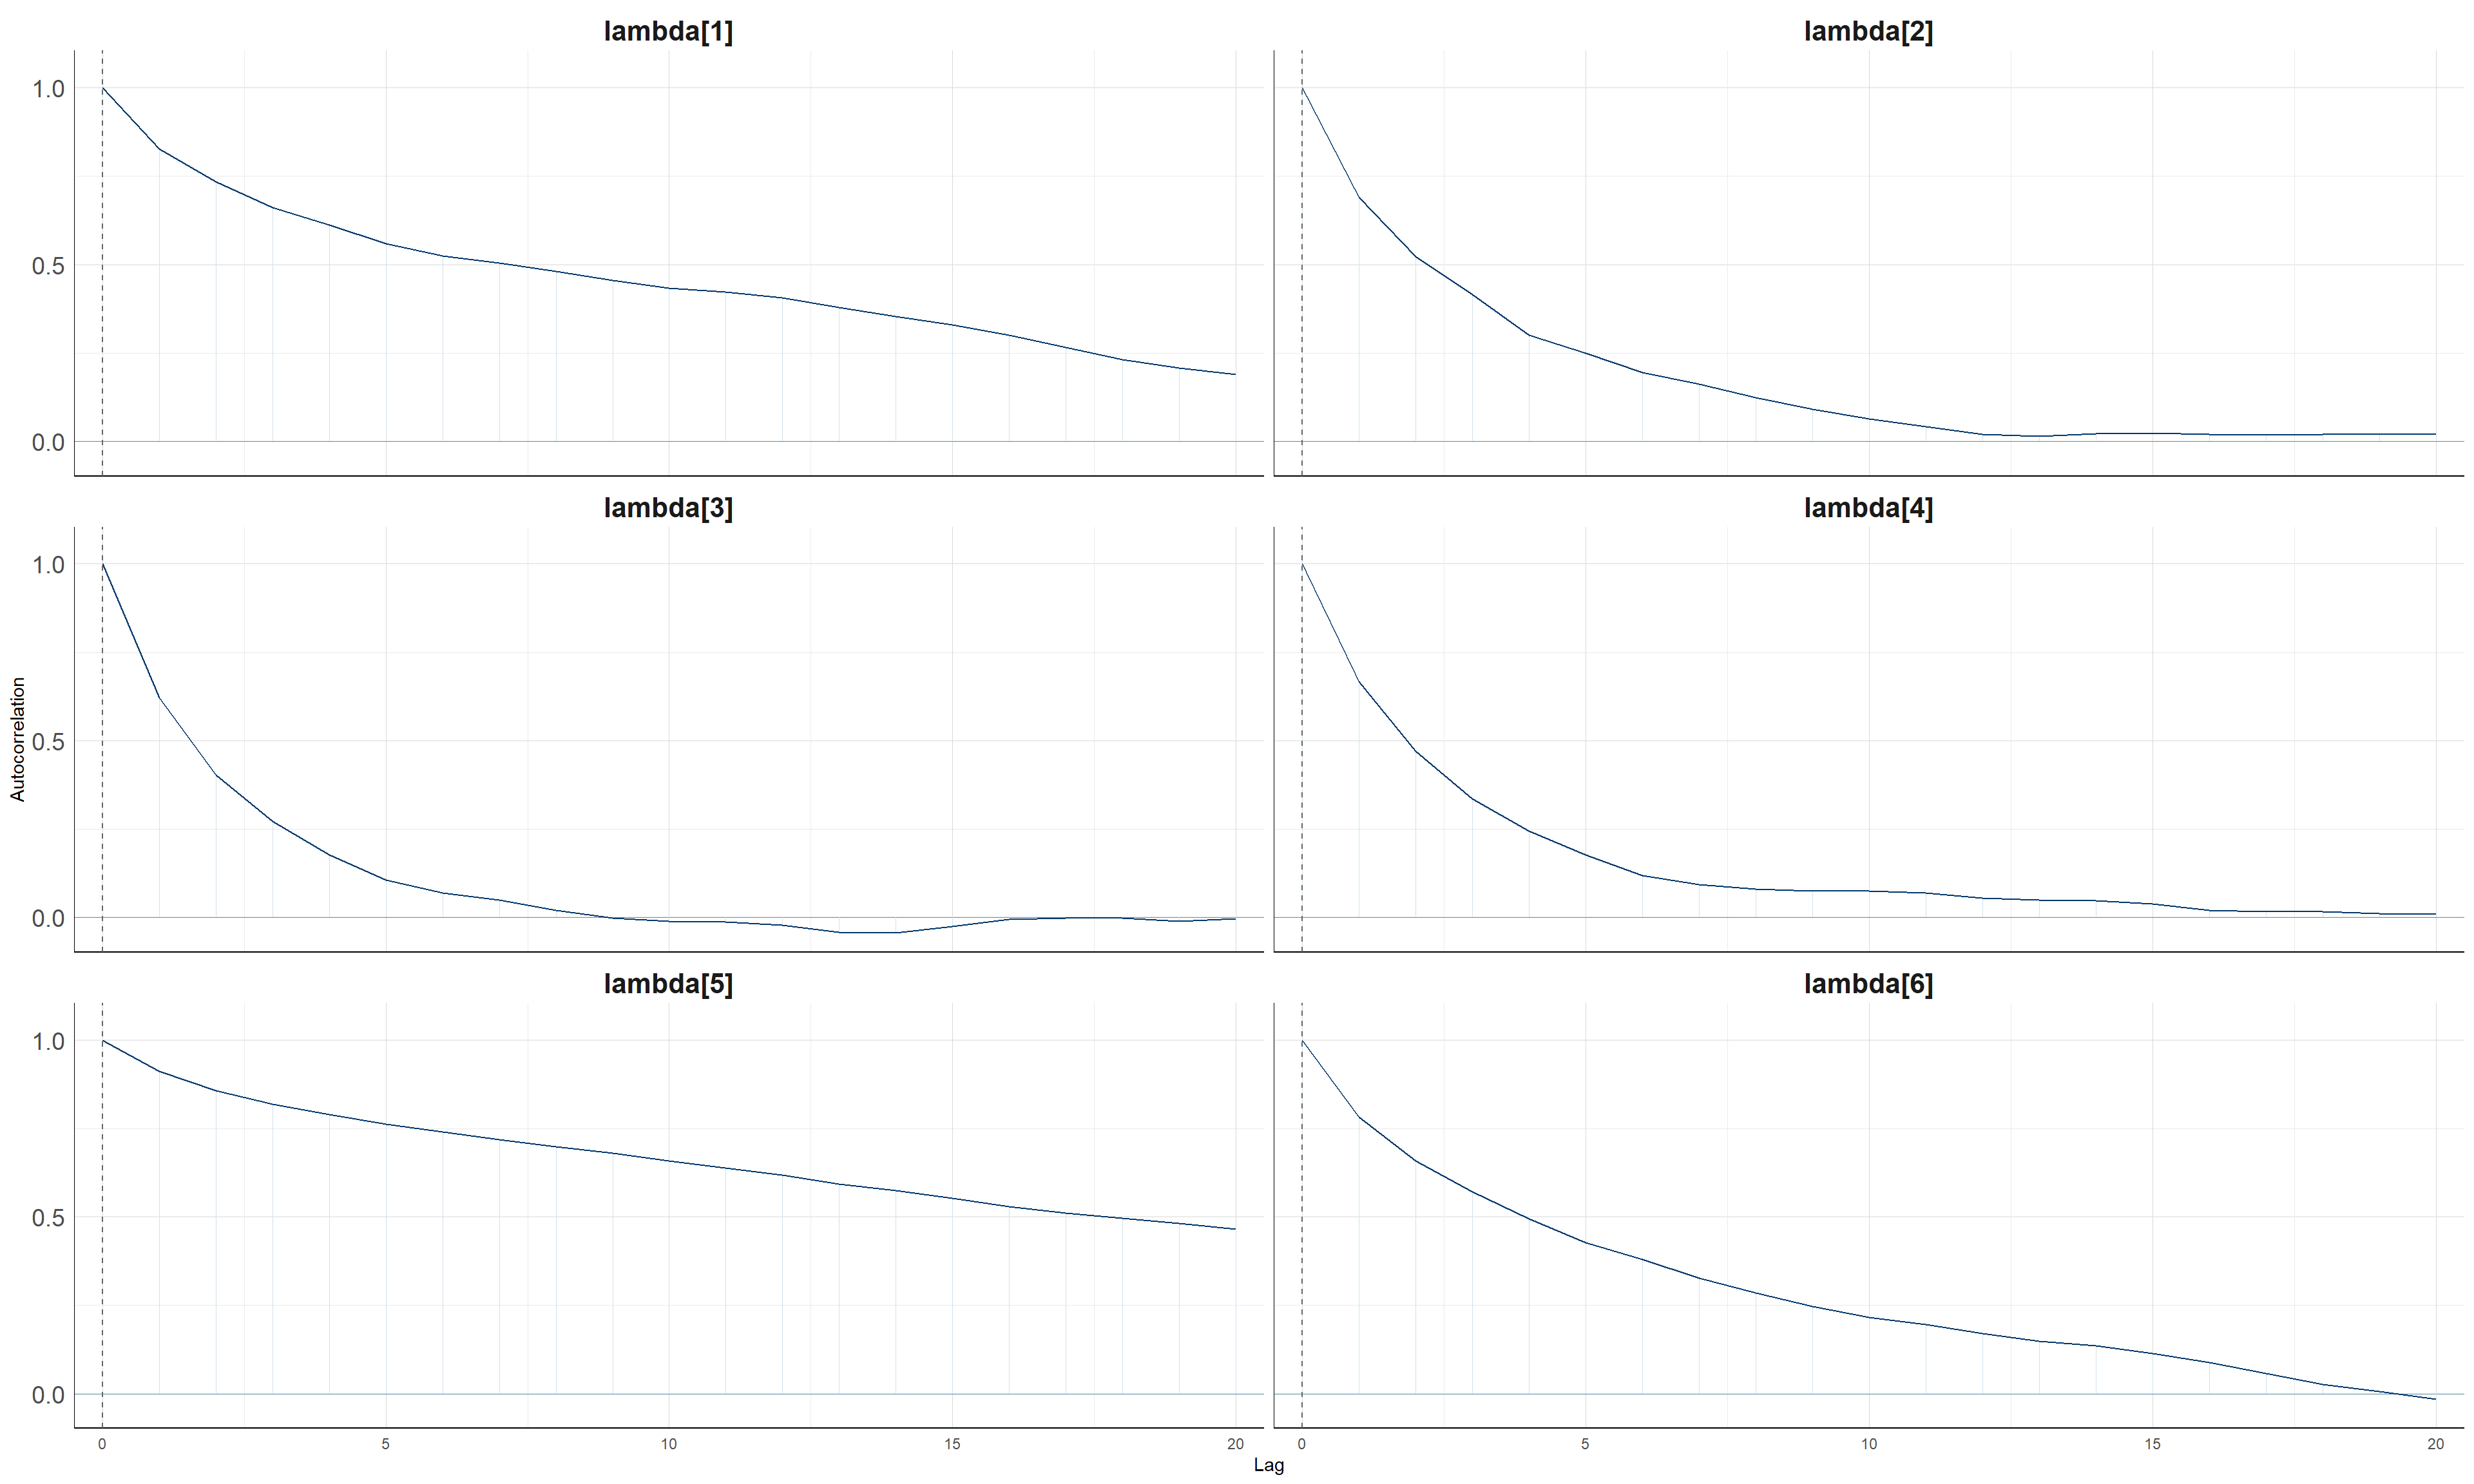
\includegraphics[width=\linewidth]{img/horseshoe_model/acf_lambda_chain3_1.png}
    \caption{Group 1.}
  \end{subfigure}\hfill
  \begin{subfigure}[t]{0.48\linewidth}
    \centering
    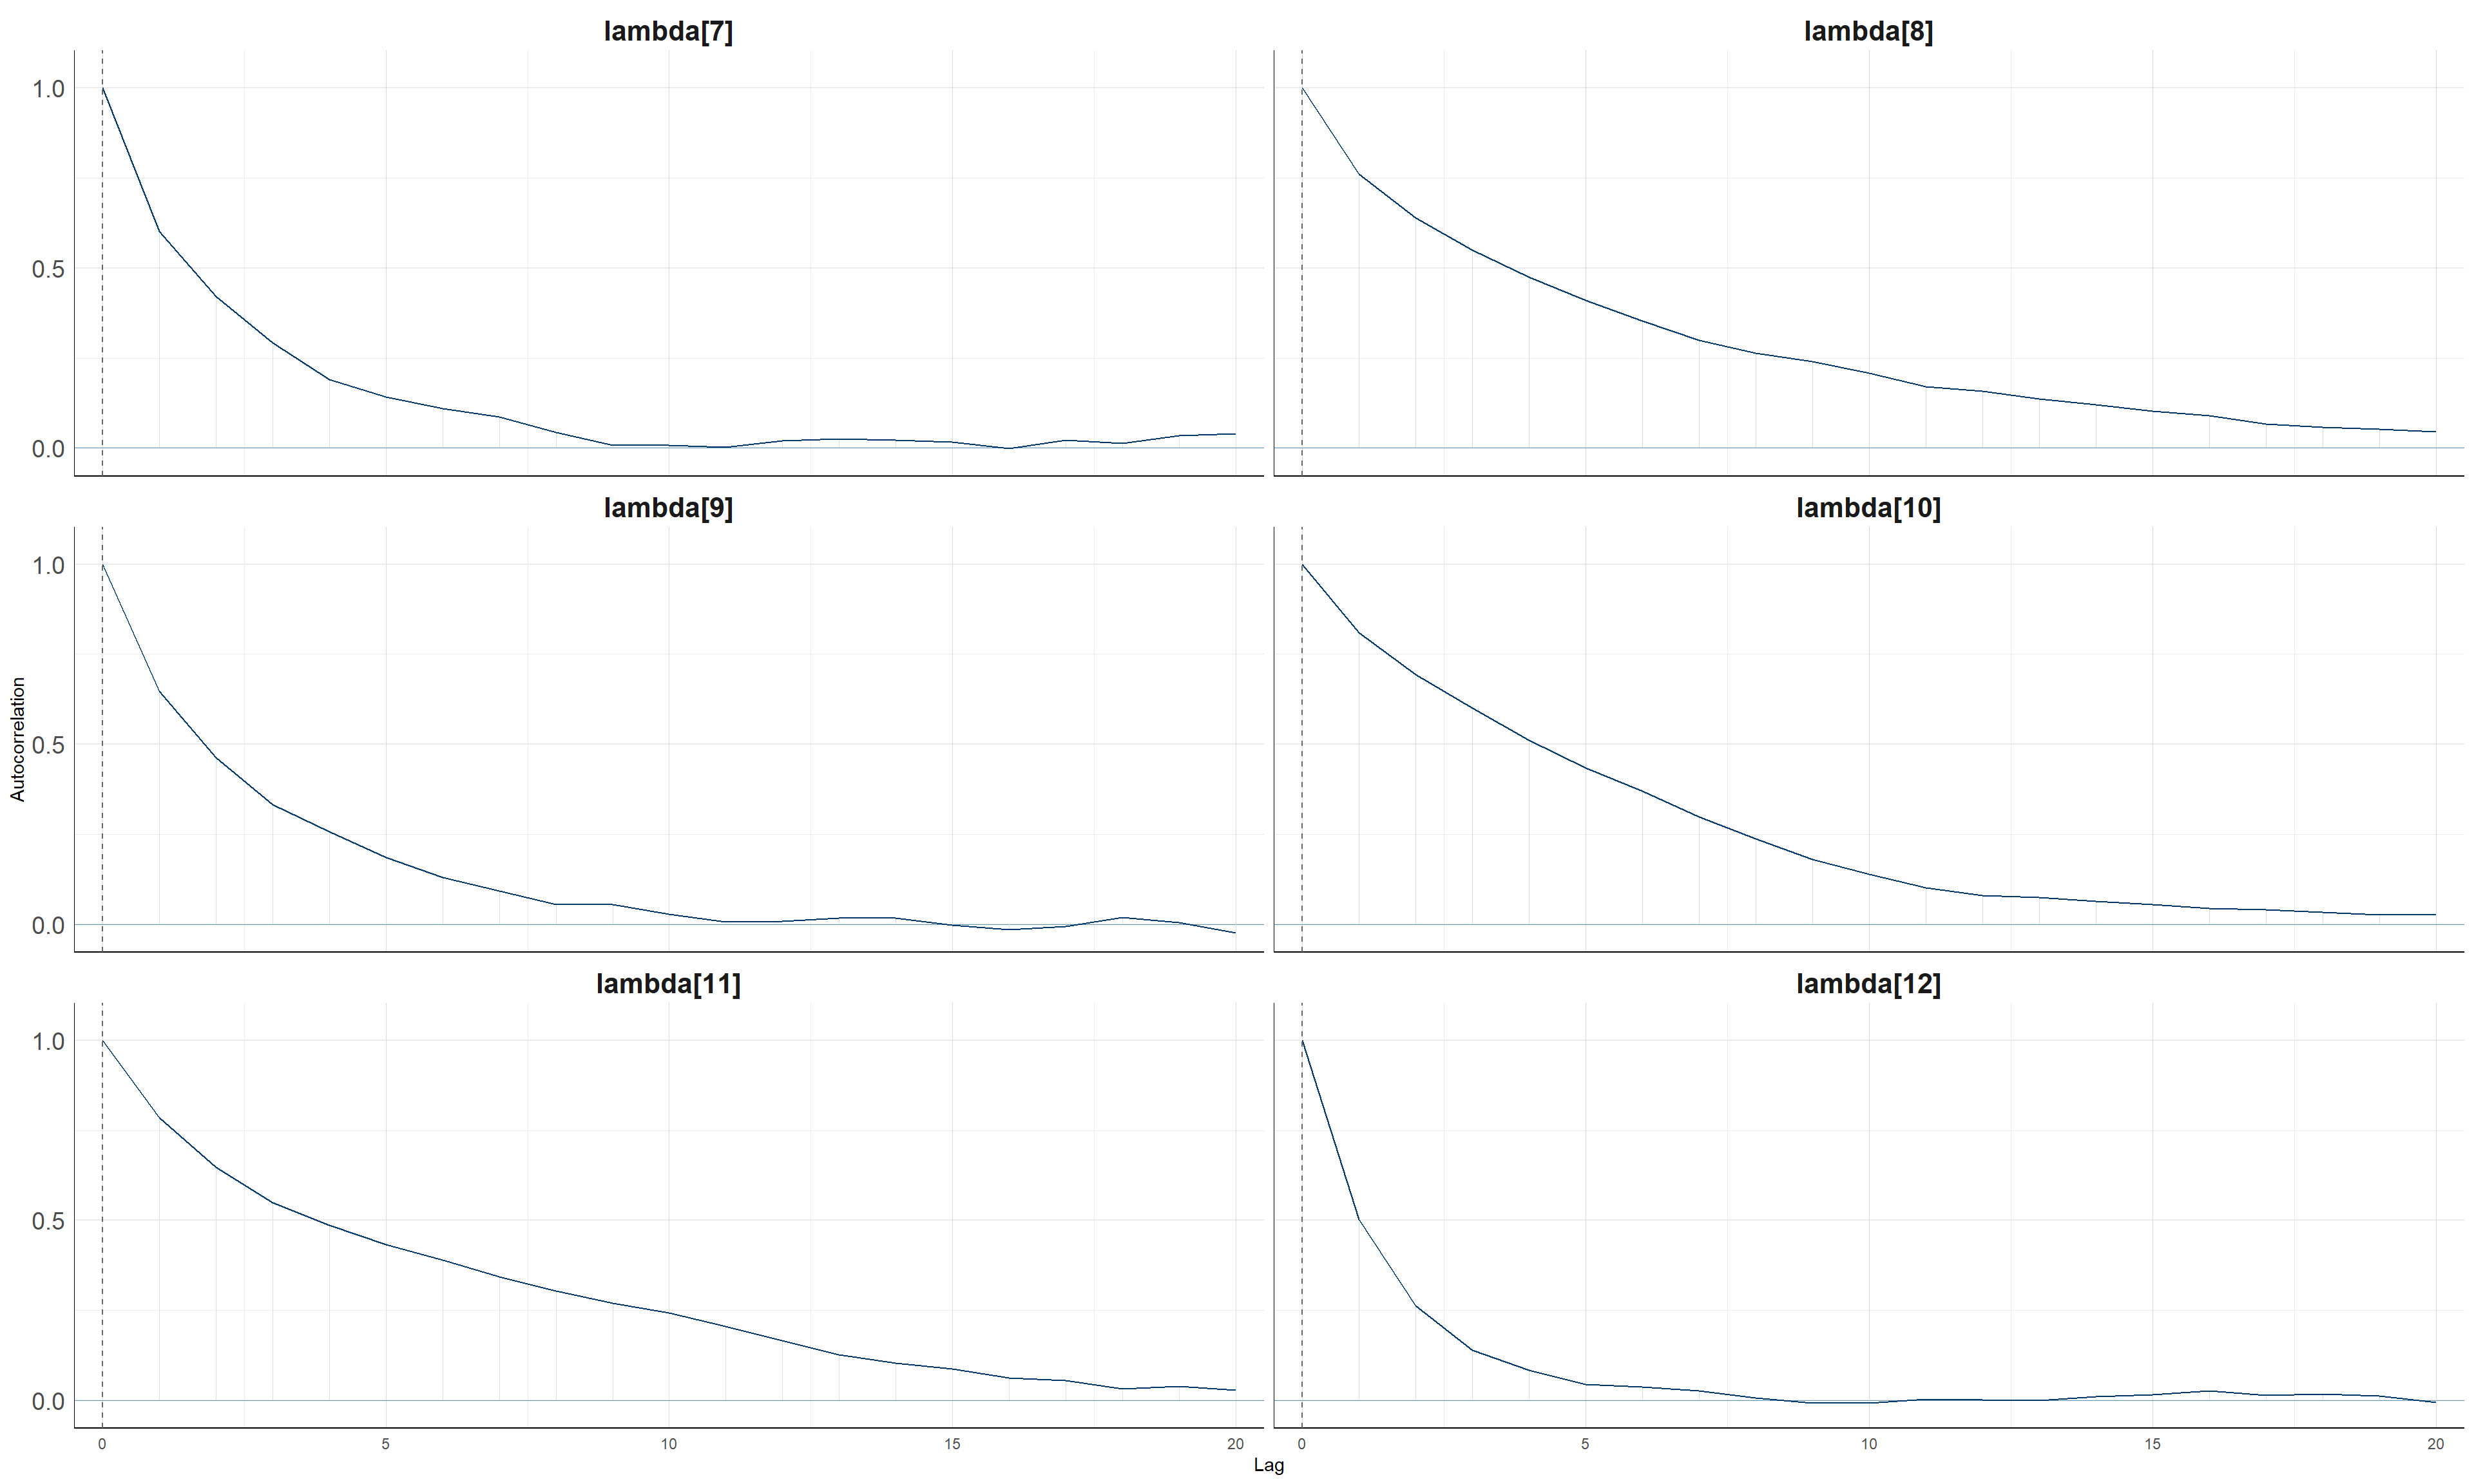
\includegraphics[width=\linewidth]{img/horseshoe_model/acf_lambda_chain3_2.png}
    \caption{Group 2.}
  \end{subfigure}\hfill
  \begin{subfigure}[t]{0.48\linewidth}
    \centering
    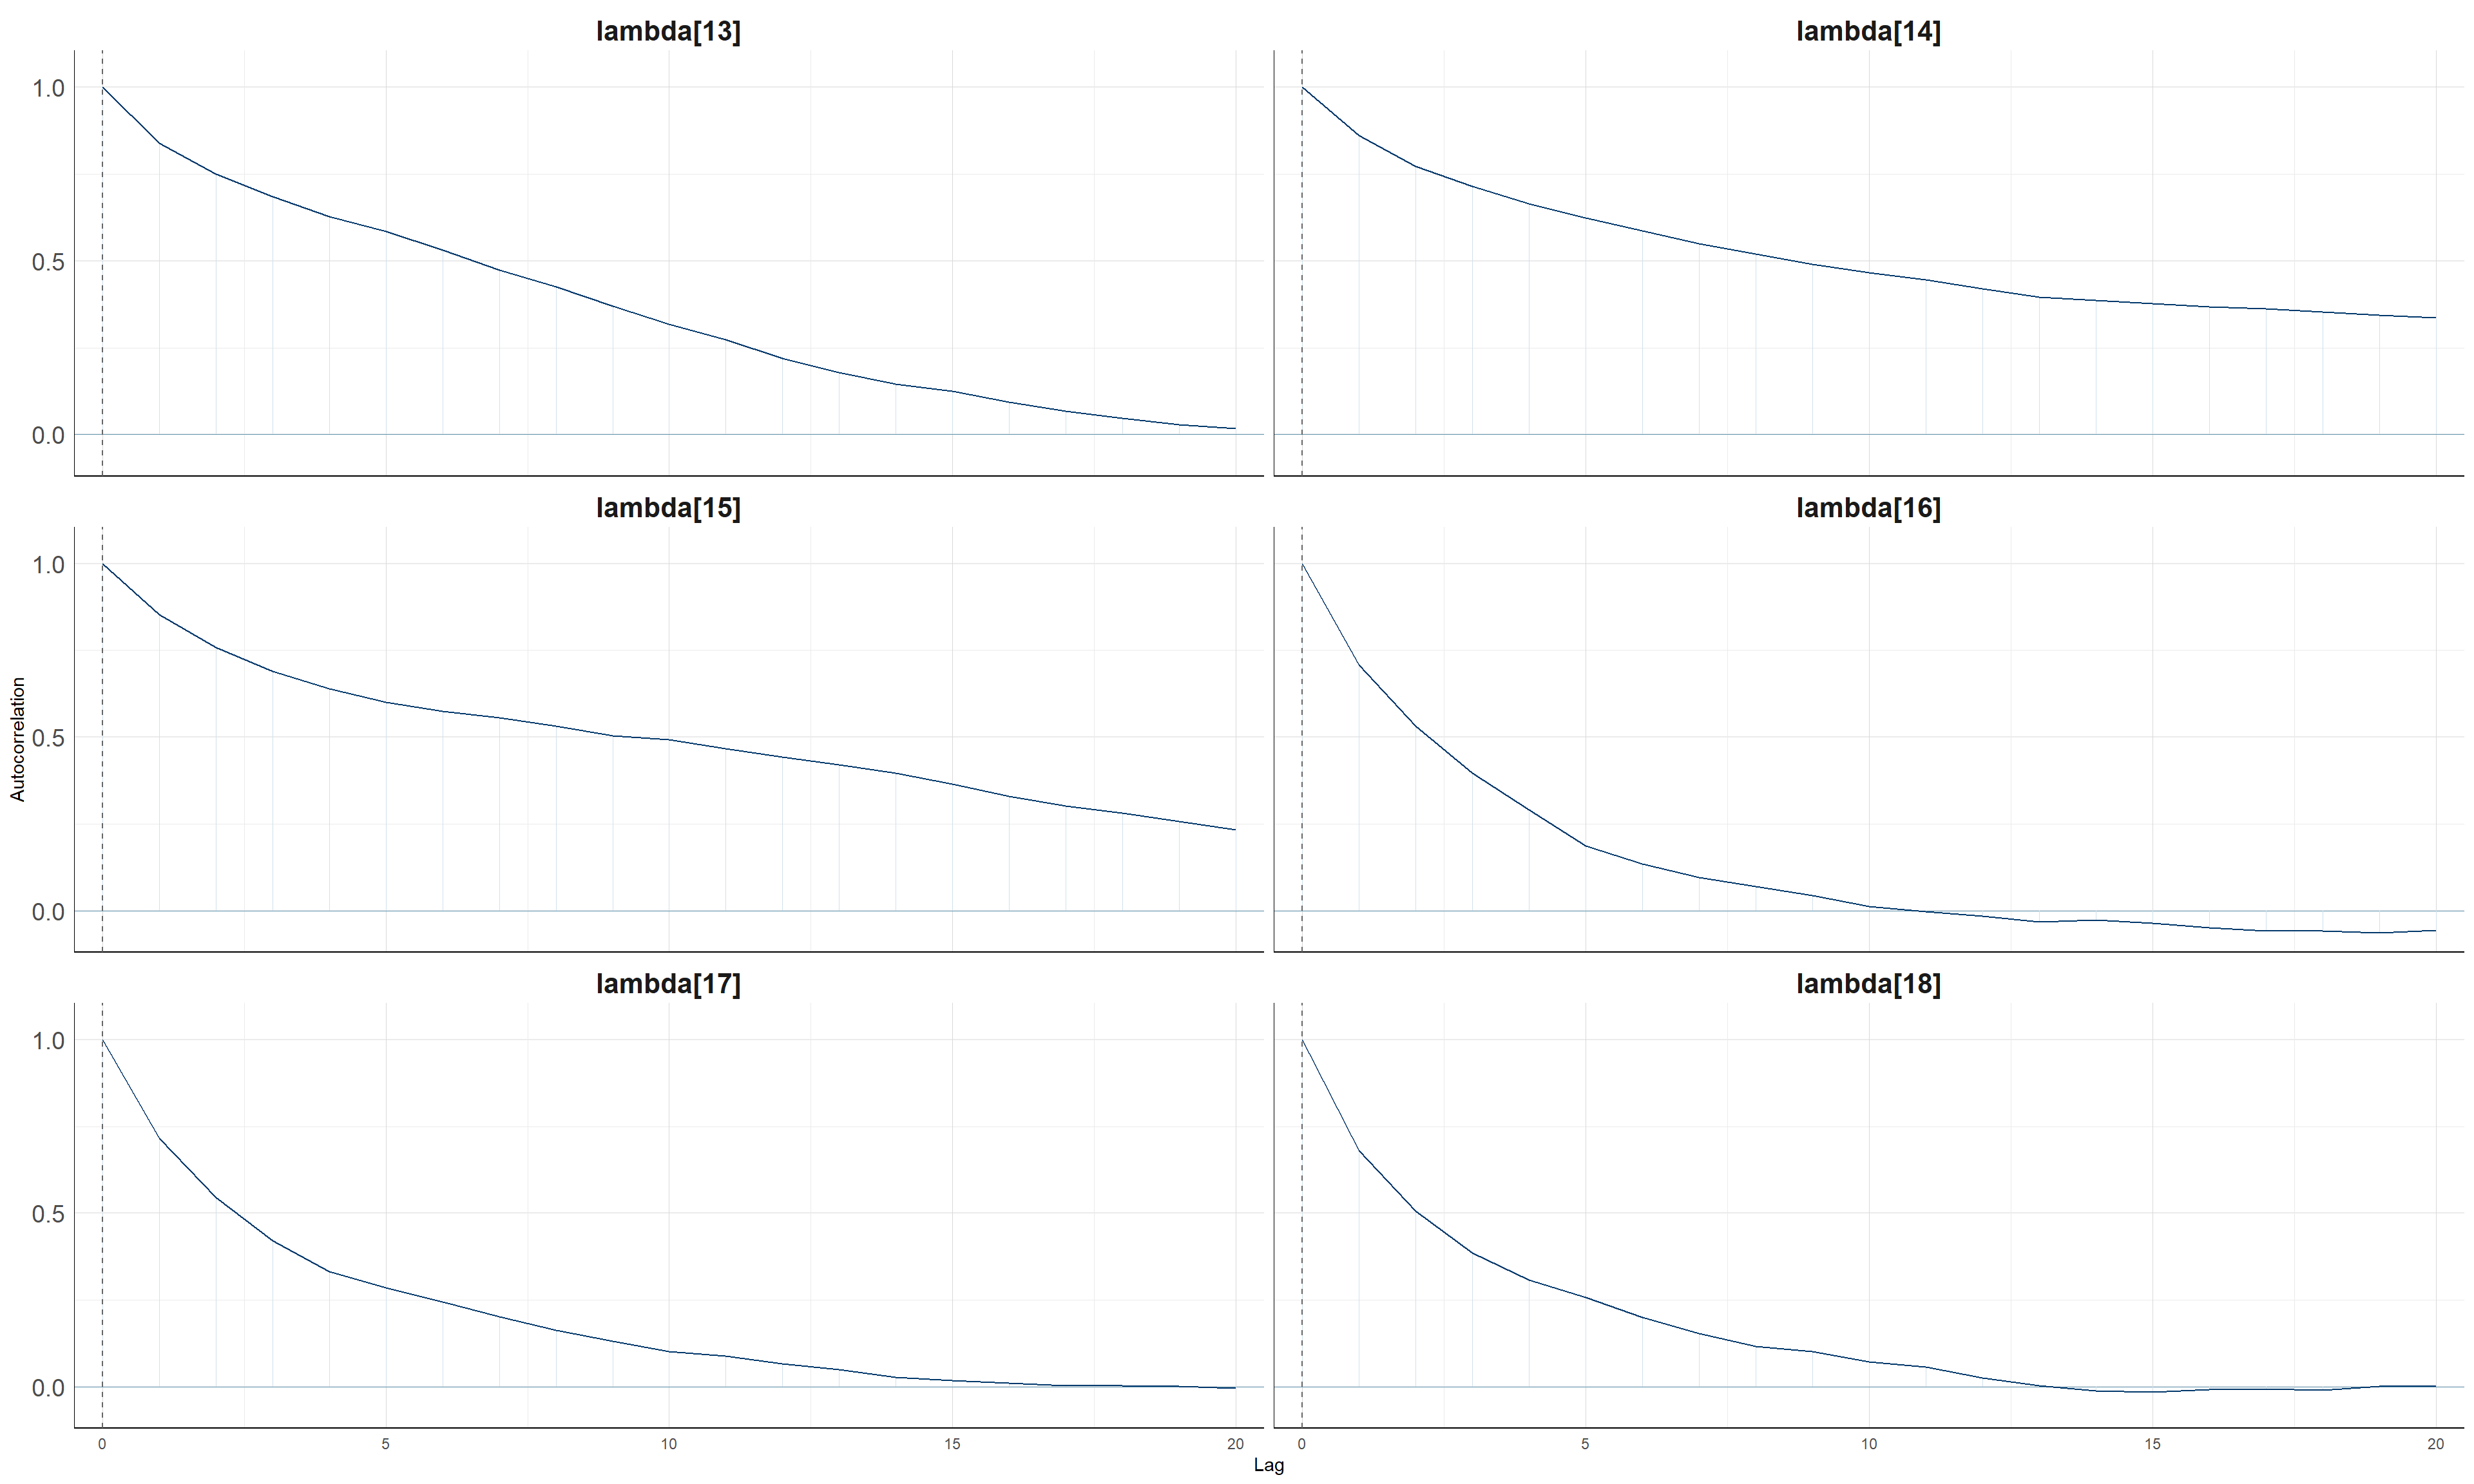
\includegraphics[width=\linewidth]{img/horseshoe_model/acf_lambda_chain3_3.png}
    \caption{Group 3.}
  \end{subfigure}\hfill
  \begin{subfigure}[t]{0.48\linewidth}
    \centering
    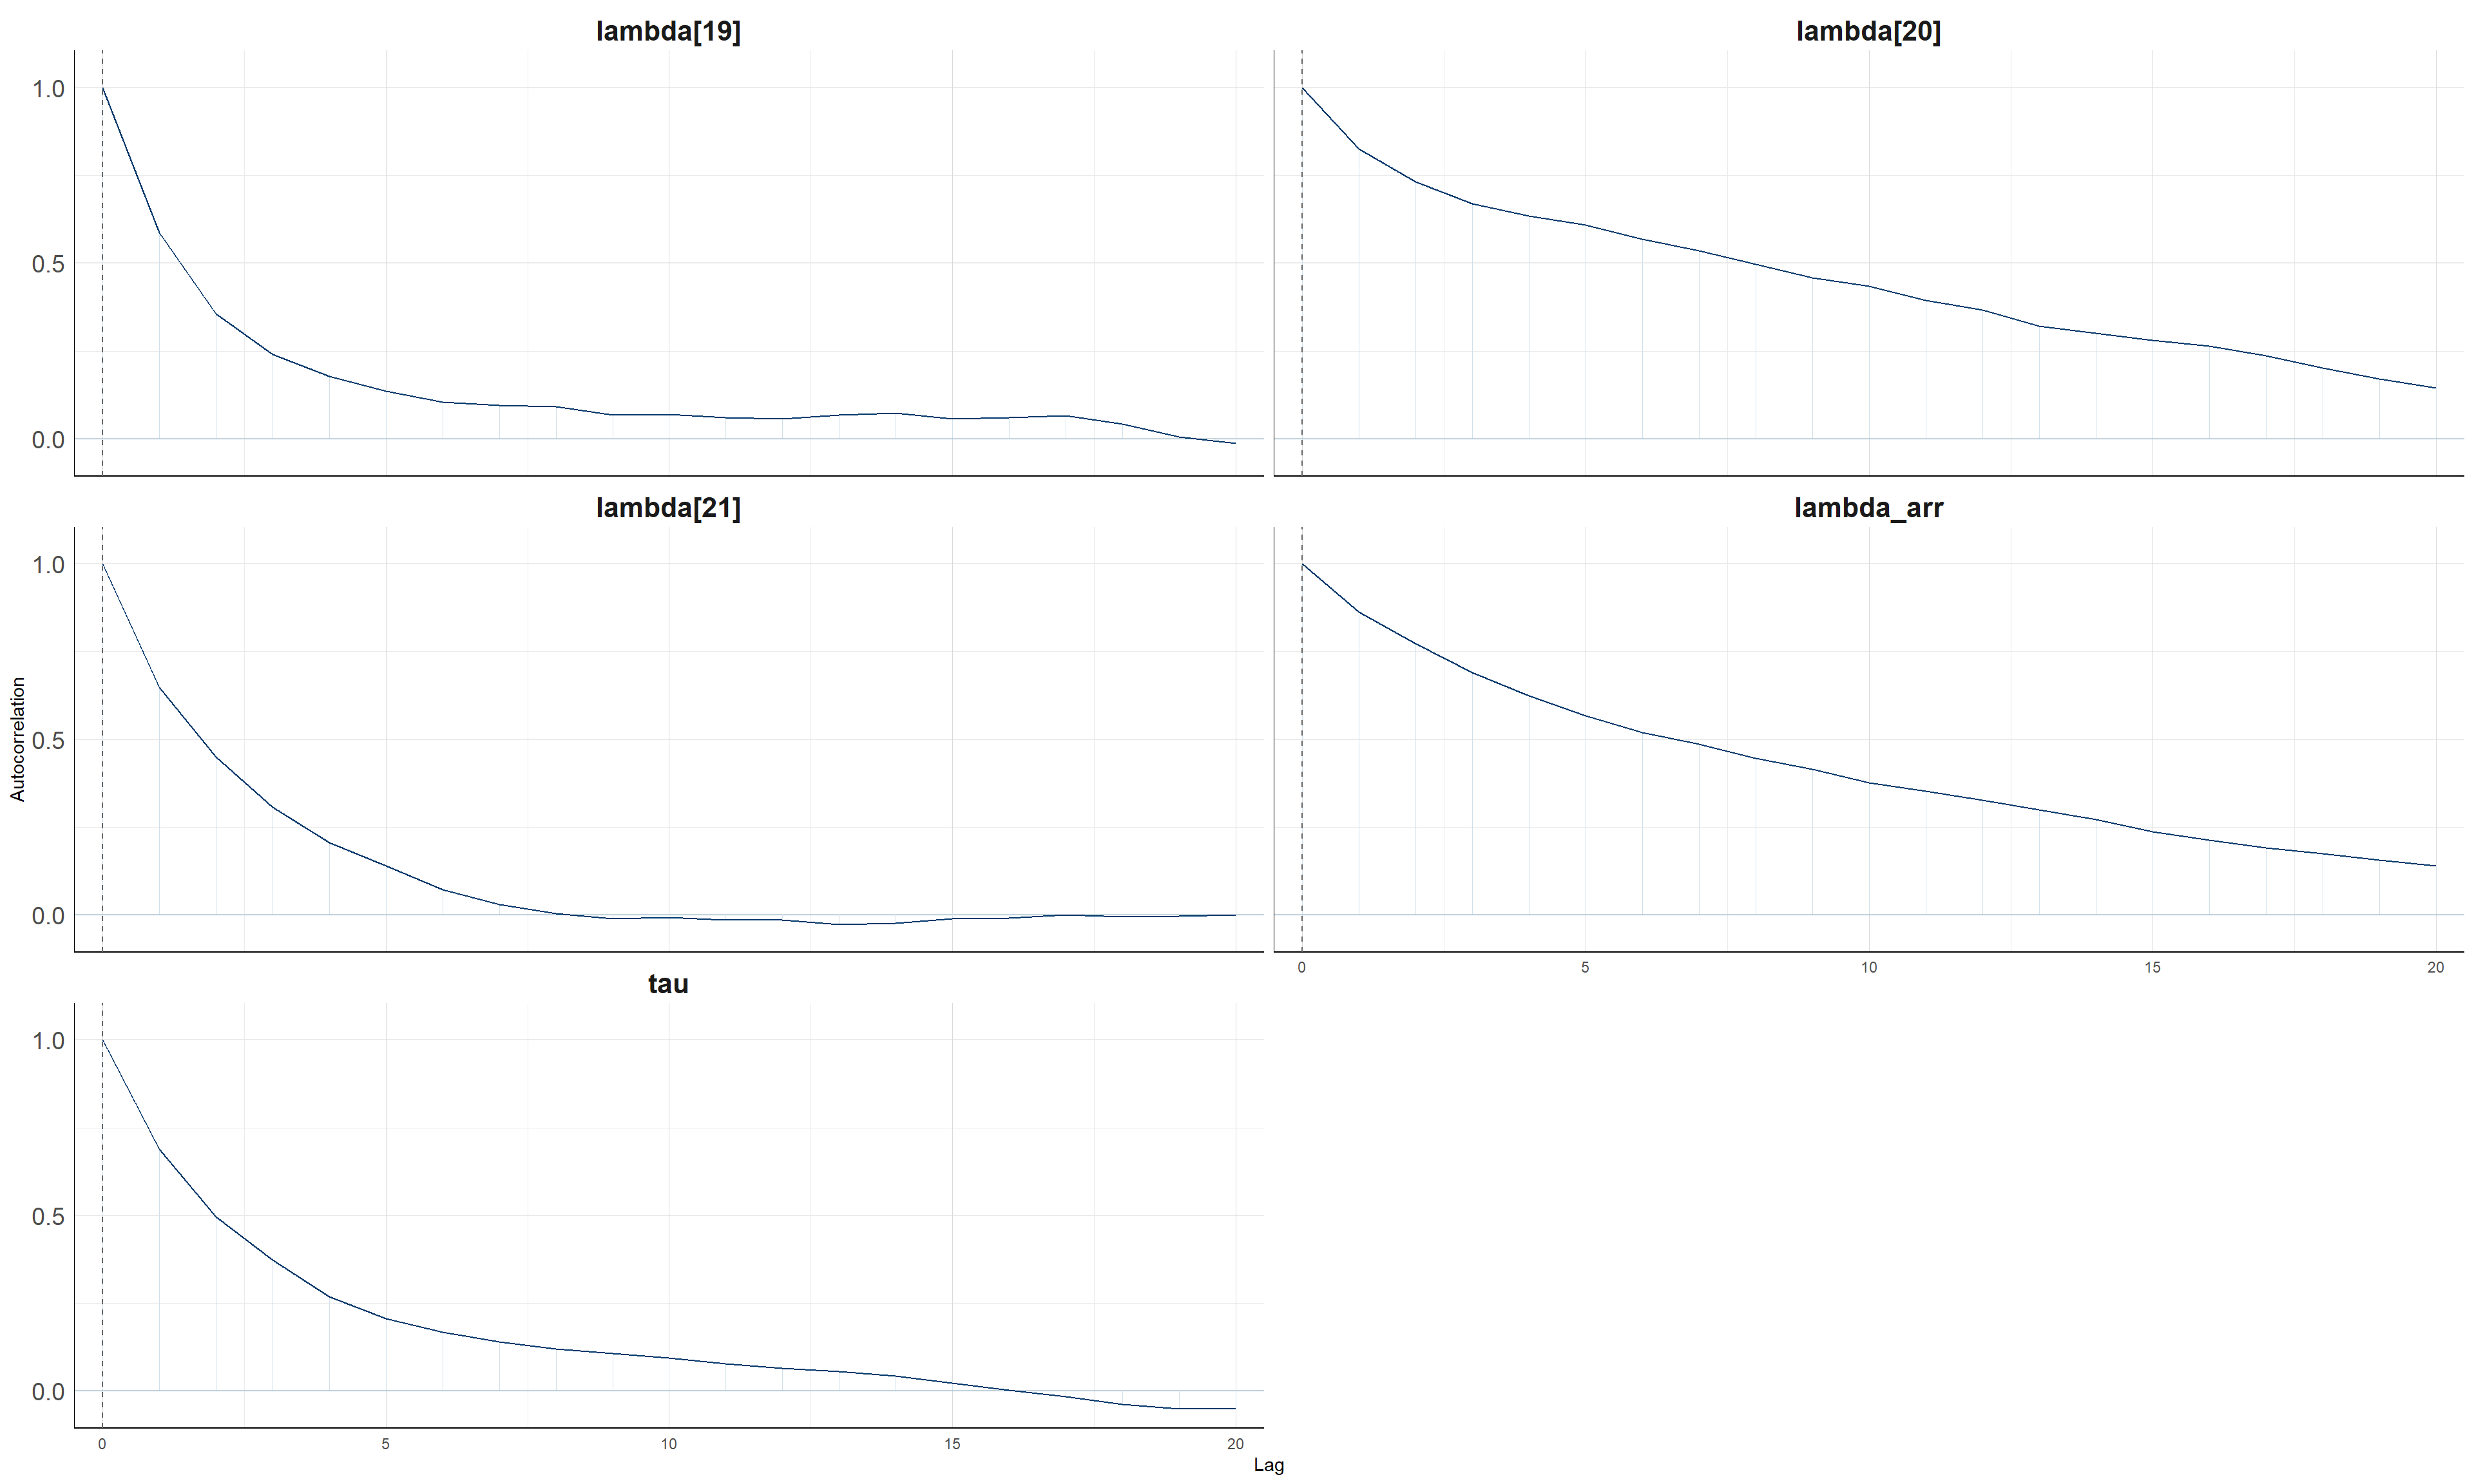
\includegraphics[width=\linewidth]{img/horseshoe_model/acf_lambda_chain3_4.png}
    \caption{Group 4.}
  \end{subfigure}\hfill
  \caption{Autocorrelation of the scales $\lambda_j$, chain 3.}
  \label{fig:hs_acf_lambda_3}
\end{figure}

\subsection*{Gelman--Rubin and effective sample sizes}
\begin{table}[htbp]
\centering\small
\caption{Regression coefficients: potential scale reduction factors and effective sample sizes.}
\label{tab:hs-psrf-beta}
\begin{tabular}{l S[table-format=1.2] S[table-format=1.2] S[table-format=5.0]}
\toprule
Parameter & {Point est.} & {Upper C.I.} & {ESS} \\
\midrule
$\beta_{1}$ (Seat comfort) & 1.00 & 1.00 & 7252 \\
$\beta_{2}$ (Dep/Arr time convenient) & 1.00 & 1.00 & 17305 \\
$\beta_{3}$ (Food and drink) & 1.00 & 1.00 & 7253 \\
$\beta_{4}$ (Gate location) & 1.00 & 1.00 & 19441 \\
$\beta_{5}$ (Inflight wifi service) & 1.00 & 1.00 & 11754 \\
$\beta_{6}$ (Inflight entertainment) & 1.00 & 1.00 & 16866 \\
$\beta_{7}$ (Online support) & 1.00 & 1.00 & 10699 \\
$\beta_{8}$ (Ease of Online booking) & 1.00 & 1.00 & 7660 \\
$\beta_{9}$ (On-board service) & 1.00 & 1.00 & 15288 \\
$\beta_{10}$ (Leg room service) & 1.00 & 1.00 & 19144 \\
$\beta_{11}$ (Baggage handling) & 1.00 & 1.00 & 11739 \\
$\beta_{12}$ (Checkin service) & 1.00 & 1.00 & 17602 \\
$\beta_{13}$ (Cleanliness) & 1.00 & 1.00 & 11220 \\
$\beta_{14}$ (Online boarding) & 1.00 & 1.00 & 12963 \\
$\beta_{15}$ (Age) & 1.00 & 1.00 & 18345 \\
$\beta_{16}$ (Flight Distance) & 1.00 & 1.00 & 23187 \\
$\beta_{17}$ (Class: Eco Plus) & 1.00 & 1.00 & 23539 \\
$\beta_{18}$ (Class: Business) & 1.00 & 1.00 & 4767 \\
$\beta_{19}$ (log(1+Departure Delay)) & 1.00 & 1.00 & 16674 \\
$\beta_{20}$ (Personal Travel) & 1.00 & 1.00 & 3813 \\
$\beta_{21}$ (disloyal Customer) & 1.00 & 1.00 & 7952 \\
$\beta_0$ (Intercept) & 1.00 & 1.00 & 3412 \\
$\beta_{\text{mid}}$ (Mid-flight delay) & 1.00 & 1.00 & 23618 \\
\bottomrule
\end{tabular}
\end{table}

\begin{table}[htbp]
\centering\small
\caption{Scale parameters: potential scale reduction factors and effective sample sizes.}
\label{tab:hs-psrf-lambda}
\begin{tabular}{l S[table-format=1.2] S[table-format=1.2] S[table-format=5.0]}
\toprule
Parameter & {Point est.} & {Upper C.I.} & {ESS} \\
\midrule
$\lambda_{1}$ (Seat comfort) & 1.01 & 1.01 & 4488 \\
$\lambda_{2}$ (Dep/Arr time convenient) & 1.02 & 1.02 & 3762 \\
$\lambda_{3}$ (Food and drink) & 1.10 & 1.12 & 1388 \\
$\lambda_{4}$ (Gate location) & 1.02 & 1.03 & 4882 \\
$\lambda_{5}$ (Inflight wifi service) & 1.03 & 1.04 & 3382 \\
$\lambda_{6}$ (Inflight entertainment) & 1.02 & 1.02 & 4499 \\
$\lambda_{7}$ (Online support) & 1.01 & 1.01 & 4077 \\
$\lambda_{8}$ (Ease of Online booking) & 1.02 & 1.03 & 2452 \\
$\lambda_{9}$ (On-board service) & 1.01 & 1.01 & 3662 \\
$\lambda_{10}$ (Leg room service) & 1.21 & 1.31 & 2103 \\
$\lambda_{11}$ (Baggage handling) & 1.03 & 1.04 & 3177 \\
$\lambda_{12}$ (Checkin service) & 1.04 & 1.05 & 3822 \\
$\lambda_{13}$ (Cleanliness) & 1.04 & 1.04 & 2497 \\
$\lambda_{14}$ (Online boarding) & 1.10 & 1.11 & 2432 \\
$\lambda_{15}$ (Age) & 1.08 & 1.11 & 2108 \\
$\lambda_{16}$ (Flight Distance) & 1.00 & 1.00 & 2753 \\
$\lambda_{17}$ (Class: Eco Plus) & 1.02 & 1.02 & 3341 \\
$\lambda_{18}$ (Class: Business) & 1.03 & 1.03 & 3262 \\
$\lambda_{19}$ (log(1+Departure Delay)) & 1.05 & 1.06 & 2458 \\
$\lambda_{20}$ (Personal Travel) & 1.01 & 1.02 & 2919 \\
$\lambda_{21}$ (disloyal Customer) & 1.05 & 1.06 & 2755 \\
$\lambda_{\text{mid}}$ (Mid-flight delay) & 1.03 & 1.04 & 3422 \\
$\tau$ (global scale) & 1.00 & 1.00 & 4515 \\
\bottomrule
\end{tabular}
\end{table}

\noindent Every coefficient has a potential scale reduction factor of
$1.00$ and an effective sample size in the thousands, the lowest being the
intercept at \num{3412}. The scale parameters are less well behaved, as
expected: their effective sample sizes run from \num{1388} to \num{4882}, and
three local scales sit at or above the conventional $1.1$ threshold ---
$\lambda_{10}$ (\emph{Leg room service}) at $1.21$ with an upper limit of
$1.31$, $\lambda_{3}$ (\emph{Food and drink}) at $1.10$, and $\lambda_{14}$
(\emph{Online boarding}) at $1.10$. We report this rather than smooth it over.
The quantity these feed into is the shrinkage weight
$\kappa_j = 1/(1+\lambda_j^2)$, which is a bounded, monotone transformation of
$\lambda_j$, and the corresponding coefficients $\beta_3$, $\beta_{10}$ and
$\beta_{14}$ have themselves converged cleanly (PSRF $1.00$, ESS \num{7253},
\num{19144} and \num{12963}). The conclusions of Section~\ref{sec:regression}
rest on the coefficients and on the broad signal/noise separation, not on the
third decimal of any single $\kappa_j$, and
Section~\ref{sec:sens-horseshoe} shows the verdicts are stable across a
hundred-fold change in the global scale. The global scale $\tau$ itself mixes
well (PSRF $1.00$, ESS \num{4515}).
